\documentclass[a4paper, 11pt, oneside]{Dissertation}
\usepackage{times}
\usepackage{iftex}
\ifXeTeX
  \usepackage{fontspec}
  \setmainfont{texgyretermes}[Extension=.otf, UprightFont=*-regular, BoldFont=*-bold, ItalicFont=*-italic, BoldItalicFont=*-bolditalic]
  \setmonofont{texgyrecursor}[Extension=.otf, UprightFont=*-regular, BoldFont=*-bold, ItalicFont=*-italic, BoldItalicFont=*-bolditalic]
\fi
\usepackage{epsfig}
\usepackage{amsmath}
\usepackage{amssymb}
\usepackage{latexsym}
\usepackage{graphicx}
\usepackage{multirow}
\usepackage[english]{babel}
\usepackage{multirow}
\usepackage{amsmath}
\usepackage{longtable}
\usepackage{algorithmicx}
\usepackage{graphicx}
\usepackage{amsmath}
\usepackage{algorithm}
\usepackage{algpseudocode}
\usepackage[numbers]{natbib}
\usepackage{array}
\usepackage{booktabs}
\usepackage{tikz}
\usepackage{pgf}
\usetikzlibrary{shapes,arrows,positioning,fit,backgrounds,calc,decorations.pathreplacing,matrix}
\usepackage{xcolor}
\usepackage{listings}
\usepackage{url}
\usepackage{tabularx}
\usepackage{hyperref}
\usepackage{float}        % enables [H] specifier - forces figure exactly here
\usepackage{placeins}     % enables \FloatBarrier - stops floats crossing sections
\usepackage{colortbl}     % enables \rowcolor in tables
% Tighten spacing around floats so figures sit closer to their reference text
\setlength{\textfloatsep}{10pt plus 2pt minus 2pt}
\setlength{\floatsep}{8pt plus 2pt minus 2pt}
\setlength{\tabcolsep}{4pt}
\setlength{\intextsep}{8pt plus 2pt minus 2pt}

% TikZ styles
\tikzstyle{block} = [rectangle, draw, fill=blue!15, text width=5em, text centered, rounded corners, minimum height=3em]
\tikzstyle{wideblock} = [rectangle, draw, fill=blue!15, text width=8em, text centered, rounded corners, minimum height=3em]
\tikzstyle{arrow} = [thick,->,>=stealth]
\tikzstyle{entity} = [rectangle, draw, fill=green!15, text width=5em, text centered, minimum height=2.5em]
\tikzstyle{process} = [rectangle, draw, fill=orange!20, text width=6em, text centered, rounded corners, minimum height=3em]
\tikzstyle{datastore} = [rectangle, draw, fill=yellow!20, text width=6em, text centered, minimum height=2.5em]
\tikzstyle{actor} = [ellipse, draw, fill=cyan!15, text width=4em, text centered, minimum height=2.5em]
\tikzstyle{dbbox} = [rectangle, draw, fill=purple!15, text width=6em, text centered, minimum height=2.5em]
\tikzstyle{fkline} = [dashed, thick, ->, >=stealth, gray]

\definecolor{codegreen}{rgb}{0,0.6,0}
\definecolor{codegray}{rgb}{0.5,0.5,0.5}
\lstdefinelanguage{JavaScript}{
  keywords={const,let,var,async,await,function,return,if,else,throw,new,for,of,in,try,catch,finally,module,require,null,true,false,typeof},
  sensitive=true, comment=[l]{//}, morecomment=[s]{/*}{*/},
  morestring=[b]', morestring=[b]", morestring=[b]`
}
\lstdefinelanguage{SQLx}{
  keywords={SELECT,FROM,WHERE,AND,OR,ORDER,BY,LIMIT,FOR,UPDATE,INSERT,INTO,VALUES,SET,DELETE,CREATE,TABLE,ALTER,ADD,COLUMN,UNIQUE,INDEX,NULL,NOT,IN,AS,DESC,ASC,ON,JOIN,IS},
  sensitive=false, comment=[l]{--}, morestring=[b]'
}
\lstset{
  basicstyle=\small\ttfamily,
  breaklines=true,
  keywordstyle=\color{blue},
  commentstyle=\color{codegreen},
  numberstyle=\tiny\color{codegray},
  frame=single,
  columns=fullflexible,
  keepspaces=true,
  showstringspaces=false
}

\newcolumntype{L}[1]{>{\raggedright\let\newline\\\arraybackslash\hspace{0pt}}m{#1}}
\newcolumntype{C}[1]{>{\centering\let\newline\\\arraybackslash\hspace{0pt}}m{#1}}
\newcolumntype{R}[1]{>{\raggedleft\let\newline\\\arraybackslash\hspace{0pt}}m{#1}}

\graphicspath{{Figures/}{./}}

\long\def\symbolfootnote[#1]#2{\begingroup%
\def\thefootnote{\fnsymbol{footnote}}\footnote[#1]{#2}\endgroup}
\renewcommand{\baselinestretch}{1.2}
\onecolumn

%% ----------------------------------------------------------------
\begin{document}
\sloppy
\pagenumbering{roman}

%%Cover Page
\thispagestyle{empty}
\begin{center}
{\Large \bf App Development for Hospital Digital Ecosystem\\}

\vspace*{1.75cm}
{\large \bf Project report submitted in partial fulfillment\\}
{\large \bf of the requirements for the degree of \\}

\vspace*{1cm}
{\it {\large Bachelor of Technology} \\
{\large by\\}}

\vspace*{1cm}
{\large \bf Prince Gupta -- Roll No. 23ucs678 -- CSE \\}
{\large \bf Sajal Jaggi -- Roll No. 23ucs695 -- CSE \\}
{\large \bf Kavya Patni -- Roll No. 23ucs615 -- CSE \\}

\vspace*{5mm}
{\large \bf Under Guidance of \\}
{\large \bf Dr. Preety Singh \\}
{\large \bf (Department of Computer Science and Engineering) \\}

\vspace*{1.0cm}
{
\includegraphics[width=44mm]{Figures/LNMIIT.png}\\}

\vspace*{2.0cm}
{\large \bf Department of Computer Science and Engineering \\}
{\large \bf The LNM Institute of Information Technology, Jaipur\\}

\vspace*{1.0cm}
{\large \bf November 2026\\}
\end{center}
\clearpage


%% COPYRIGHT PAGE
\newpage
\thispagestyle{empty}
\vspace*{12cm}
\begin{center}
Copyright \copyright\ The LNMIIT 2026\\
All Rights Reserved
\end{center}
\clearpage


%% CERTIFICATE PAGE
\newpage
\thispagestyle{empty}
\vspace*{1.5cm}
\begin{center}
{\Large The LNM Institute of Information Technology\\}
{\Large Jaipur, India\\}
\vspace*{3cm}
{\Large \bf CERTIFICATE\\}
\vspace*{1cm}
\noindent
\end{center}
This is to certify that the project entitled \textbf{``App Development for Hospital Digital Ecosystem''}, submitted by Prince Gupta (Roll No. 23ucs678), Sajal Jaggi (Roll No. 23ucs695) and Kavya Patni (Roll No. 23ucs615) in partial fulfillment of the requirement of degree in Bachelor of Technology (B.~Tech), is a bonafide record of work carried out by them at the Department of Computer Science and Engineering, The LNM Institute of Information Technology, Jaipur, (Rajasthan) India, during the academic session 2026--2027 under my supervision and guidance and the same has not been submitted elsewhere for award of any other degree. In my opinion, this report is of the standard required for the award of the degree of Bachelor of Technology (B.~Tech).

\vspace*{3cm}
\begin{tabular}{cc}
\underline{\makebox[1in]{}} & \hspace*{5cm} \underline{\makebox[2.5in]{}} \\
Date & \hspace*{5cm} Adviser: Dr. Preety Singh
\end{tabular}


% ACKNOWLEDGEMENTS PAGE
\chapter*{Acknowledgments}
\label{ch:ack}
First and foremost, we would like to extend our sincere thanks to our project guide, Dr. Preety Singh, for the valuable guidance and support given to us throughout this project. The constant encouragement and suggestions we received played a significant role in helping us extend the system from its first version into the complete hospital platform described in this report.

Secondly, we would like to express our thanks and gratitude to all the professors and teaching staff of the Department of Computer Science and Engineering, The LNM Institute of Information Technology, Jaipur for giving us the required facilities to conduct this study.

We would like to thank our fellow batch-mates and friends for giving us moral support, suggesting ideas and creating an atmosphere of collaboration, and for testing the application and reporting the problems they found.

Also, we would like to acknowledge our seniors for playing a major part in helping us through this project.

Last but not least, we would like to thank our parents for their constant support throughout our undergraduate studies.


% Abstract
\chapter*{Abstract}
\label{ch:abs}
Hospital management is a highly significant domain because it brings together patients, medical specialists, hospital staff and clinical data. Without proper software and databases, paper-based management leads to conflicts between people, a poor patient experience and inefficient operations. This report presents \textbf{Care \& Cure HMS}, a full-stack Hospital Management System built with React.js, TypeScript, Node.js, Express.js and MySQL, and describes how the first version of the system has been extended into a complete hospital digital ecosystem.

The first version provided a role-based structure for three types of users, namely \textbf{Patients}, \textbf{Doctors} and \textbf{Administrators}. Patients register, maintain health profiles, book specialization-based appointments from real-time slots and download prescriptions. Doctors manage their appointments and upload prescriptions. Administrators manage users, doctors, appointments and slots. \textbf{MediBot}, a chatbot built on the Google Gemini API, guides patients from their symptoms to the right specialist and books appointments in conversation.

In this phase, seven new modules have been designed, implemented and tested: (1) a \textbf{Blood Bank} with donor records, ABO/Rh-compatible issue and first-expiry-first-out stock; (2) \textbf{Bed Management} in which doctors request beds and discharges and the administrator assigns them, guarded against double allocation at the database level; (3) \textbf{Emergency Management} using the five-level Emergency Severity Index (ESI) for triage; (4) \textbf{Teleconsultation} through video rooms with a timed join window, a waiting room from which the doctor admits the patient, and signed room tokens; (5) in-app \textbf{Notifications and Alerts}; (6) \textbf{Hospital Navigation} that computes shortest and wheelchair-accessible indoor routes with Dijkstra's algorithm; and (7) \textbf{Online Payments} through Razorpay with HMAC-SHA256 signature verification and idempotent webhooks.

Security has also been strengthened. Tokens now live in httpOnly cookies with short-lived access tokens and refresh-token rotation, every state-changing request is protected by a CSRF double-submit token, all inputs are validated with Zod schemas, failed logins are rate-limited per address and per account, and uploaded medical files are stored in the database and served only to their patient and doctor. Appointments can be cancelled by any party, which frees the slot and flags paid visits for refund. The database has grown from six to twenty-one tables. The system is verified by 383 automated tests (165 backend unit, 80 backend integration against a real MySQL database, 126 frontend component and contract tests, and 12 browser end-to-end tests), and runs in a GitHub Actions pipeline. It is deployed with Docker on Render, with the frontend on Vercel and the database on managed MySQL.


\pagestyle{fancy}
%--------------------------------------------------------
\tableofcontents
\listoffigures
\listoftables

% List of Abbreviations
\chapter*{List of Abbreviations}
\addcontentsline{toc}{chapter}{List of Abbreviations}
\lhead{\emph{List of Abbreviations}}
\begin{longtable}{L{2.6cm}L{11cm}}
\textbf{ABO/Rh} & Blood group systems (A, B, AB, O and Rhesus D) \\
\textbf{API} & Application Programming Interface \\
\textbf{BLOB} & Binary Large Object \\
\textbf{CI} & Continuous Integration \\
\textbf{CORS} & Cross-Origin Resource Sharing \\
\textbf{CRUD} & Create, Read, Update, Delete \\
\textbf{CSRF} & Cross-Site Request Forgery \\
\textbf{DFD} & Data Flow Diagram \\
\textbf{E2E} & End-to-End (testing) \\
\textbf{EHR} & Electronic Health Record \\
\textbf{ER} & Emergency Room (Chapter 5) / Entity-Relationship (Chapter 3) \\
\textbf{ESI} & Emergency Severity Index \\
\textbf{FEFO} & First-Expiry, First-Out \\
\textbf{FHIR} & Fast Healthcare Interoperability Resources \\
\textbf{HMAC} & Hash-based Message Authentication Code \\
\textbf{HMS} & Hospital Management System \\
\textbf{HSTS} & HTTP Strict Transport Security \\
\textbf{INR} & Indian Rupee \\
\textbf{JaaS} & Jitsi as a Service (8x8) \\
\textbf{JWT} & JSON Web Token \\
\textbf{LLM} & Large Language Model \\
\textbf{OPD} & Out-Patient Department \\
\textbf{ORM} & Object-Relational Mapping \\
\textbf{RBAC} & Role-Based Access Control \\
\textbf{REST} & Representational State Transfer \\
\textbf{RS256} & RSA signature with SHA-256 (JWT algorithm) \\
\textbf{SPA} & Single-Page Application \\
\textbf{SpO\textsubscript{2}} & Peripheral oxygen saturation \\
\textbf{SQL} & Structured Query Language \\
\textbf{TTL} & Time To Live \\
\textbf{TZ} & Time Zone \\
\textbf{XSS} & Cross-Site Scripting \\
\end{longtable}

\newpage

%% ----------------------------------------------------------------
\mainmatter

\chapter{Introduction}
\label{ch:intro}
\lhead{\emph{Chapter 1: Introduction}}
\FloatBarrier
\section{Background and Motivation}

Healthcare service providers around the world have come under increasing pressure to be efficient and error-free. With conventional management practices involving the use of pen-and-paper records, telephone calls, and manual scheduling becoming inadequate in today's fast-paced healthcare environment, there has been an evolution of web-based Hospital Management Systems (HMS). HMS systems help hospitals manage patient registration, appointment scheduling, medical history, medication dispensation, and other administrative tasks using a unified interface.

Today, HMS solutions leverage artificial intelligence to provide a seamless experience to patients. AI-driven chatbots act as assistants to patients by guiding them in understanding their symptoms and making appointments without requiring any human interaction.

Care and Cure HMS is a complete hospital management solution with modern web architecture, role-based access control, and an AI-enabled conversational assistant named MediBot.

The first version of Care \& Cure HMS concentrated on the out-patient journey: finding a doctor, booking a slot, consulting, and receiving a prescription. A real hospital, however, runs many other services in parallel. Blood must be collected, stored and issued safely; beds must be allocated and released; emergency arrivals must be prioritised by clinical urgency rather than arrival order; patients increasingly expect video consultations and online payment; and first-time visitors need help finding their way inside a large building. In the absence of a shared digital platform these services are typically run on registers, whiteboards and phone calls, which makes them slow, error-prone and impossible to audit. The motivation for the second phase of this project was therefore to grow Care \& Cure HMS from an appointment system into a \emph{hospital digital ecosystem} in which all of these services share one database, one security model and one user interface.

\FloatBarrier
\section{Problem Statement}

Even though commercially available HMS systems exist, there are various shortcomings associated with their deployment, including:

\begin{enumerate}
    \item \textbf{Disjointed workflows}: There exist many HMS systems that cater only to either patients or administrators but not both. Few HMS systems offer a seamless experience for all the involved participants: patients, doctors, and administration.
    \item \textbf{Non-dynamic appointment scheduling}: Fixed slots with manual appointment booking result in ineffective appointments, especially in a busy OPD scenario.
    \item \textbf{Absence of AI help}: Patients might be unaware about the required medical specialty to see for their issues. Absence of guidance leads to inappropriate booking by the patients and loss of valuable time from both parties.
    \item \textbf{Absence of role enforcement}: Role-based access is rarely present in many lightweight HMS deployments, hence exposing sensitive data to various risks.
    \item \textbf{Inefficient prescription management}: Many free HMS applications do not include features such as electronic prescriptions, file upload/download facilities.
    \item \textbf{Manual blood bank records}: Stock is tracked on paper, expiry dates are missed, and the compatibility of a donor unit with a recipient is checked by hand, which risks both wastage and unsafe transfusion.
    \item \textbf{No real-time bed visibility}: Ward occupancy is known only to the ward staff, so admitting doctors call around for a free bed, and the same bed can be promised to two patients.
    \item \textbf{First-come, first-served emergency queues}: Without a standard triage scale, a critically ill patient may wait behind patients with minor complaints.
    \item \textbf{No remote consultation or online payment}: Patients must travel for every consultation and queue at the reception desk to pay consultation fees.
    \item \textbf{No timely alerts and poor wayfinding}: Patients and staff are not told when something relevant happens (a booking, an admission, a critical arrival), and visitors lose time finding departments in a multi-floor building.
\end{enumerate}

\FloatBarrier
\section{Objectives}

The primary objectives of this project are:

\begin{enumerate}
    \item Development of an application that will be able to handle three roles, namely Patient, Doctor, and Administrator.
    \item Development of a dynamic and flexible scheduler which will show availability of appointment slots in real-time, specialization filters for doctors and avoids double booking.
    \item Developing a cron job to automatically generate slots based on time periods such that it will create 14 days slots for each and every registered doctor.
    \item Integrating MediBot with Google Gemini functionalities that will be able to help in symptoms assessment and also recommend suitable doctors, and allow appointment booking.
    \item Implementing a security module for the whole project using JWT (JSON Web Token) and bcrypt for password hashing.
    \item Prescription Upload module that allows doctors to upload prescriptions made for patients which patients can access later.
    \item Allowing full management of user accounts for patients and doctors, appointments, and slot details by administrators.
    \item Proving normalization of the project database which has at least five tables and constraints for integrity.
\end{enumerate}

The objectives added in the second phase are:

\begin{enumerate}
    \setcounter{enumi}{8}
    \item A \textbf{Blood Bank} module that records donors and donations, enforces the minimum interval between donations, computes component expiry, and issues only ABO/Rh-compatible units in first-expiry-first-out order.
    \item A \textbf{Bed Management} module with wards, beds, admissions and discharges, in which doctors request beds and discharges and the administrator assigns them, and the database itself prevents a bed or a patient from having two open allocations.
    \item An \textbf{Emergency Management} board that triages arrivals with the five-level Emergency Severity Index (ESI), orders the queue by severity, enforces valid status transitions, and admits patients directly into a bed.
    \item A \textbf{Teleconsultation} facility in which a patient can book a video appointment, wait in a virtual waiting room, and be admitted by the doctor to a private video room within a fixed window around the appointment time.
    \item An in-app \textbf{Notifications and Alerts} service that informs patients and staff of bookings, admissions, payments and critical emergency arrivals.
    \item A public \textbf{Hospital Navigation} feature that computes the shortest indoor route between two locations, including a step-free route for wheelchair users.
    \item An \textbf{Online Payment} module using the Razorpay gateway in which the amount is always taken from the server, every payment is verified with an HMAC-SHA256 signature, and webhooks are processed exactly once.
    \item Hardening of the platform with cookie-based sessions, CSRF protection, schema validation, rate limiting and caching, and verification of all of the above with an automated unit, integration and end-to-end test suite running in continuous integration.
\end{enumerate}

\FloatBarrier
\section{Scope of the Project}

\textbf{WITHIN THE PROJECT'S SCOPE:}
\begin{itemize}
    \item Self-registration of patients, patient profile management, and appointment history of patients.
    \item Management of doctor profiles (created by the administrator), scheduling of doctors, and prescription upload by doctors.
    \item Control Panel of the administrator managing all entities like users, doctors, appointments, and slots.
    \item Chatbot for guiding patients on symptoms and booking appointments.
    \item Automated appointment slots and cleanup of appointment slots using scheduled cron jobs.
    \item Backend with RESTful APIs with JWT authentication and authorization based on roles.
    \item Blood bank inventory, donors, donations, blood requests and compatible issue.
    \item Ward and bed management with doctor requests, admission and discharge.
    \item Emergency department case board with ESI triage and direct admission.
    \item Video teleconsultation for appointments booked as video visits, with a waiting room.
    \item In-app notifications with unread counts.
    \item Indoor navigation across floors with an accessible-route option.
    \item Online payment of consultation fees, cancellation with refund flagging, an admin payments ledger, and a patient payment history.
\end{itemize}

\textbf{OUT OF THE PROJECT'S SCOPE:}
\begin{itemize}
    \item Integration with any external EHR system.
    \item Native mobile app.
    \item Management of lab tests and radiology reports.
    \item E-mail and SMS delivery of notifications (notifications are in-app only).
    \item In-patient billing for bed charges, pharmacy and procedures (only consultation fees are collected online), and automatic refunds (refunds are flagged and issued from the gateway dashboard).
    \item Clinical decision support beyond the ESI triage suggestion; the final triage level is always chosen by the clinician.
\end{itemize}

Payment gateway integration and video consultation, which were listed as out of scope in the first version, have been brought into scope and implemented in this phase.

\FloatBarrier
\section{Technology Overview}

The system is built on a three-tier architecture using a modern JavaScript ecosystem:

\begin{itemize}
    \item \textbf{Frontend}: React.js (v19) with TypeScript, the Vite build tool, Tailwind CSS v4 for styling, React Router v7 for client-side navigation, and Axios for API communication.
    \item \textbf{Backend}: Node.js (v20) with Express.js v5, organized into RESTful route, controller, service and validator modules.
    \item \textbf{Database}: MySQL with the \texttt{mysql2} driver, using connection pooling for performance and an automatic schema migration step on start-up.
    \item \textbf{Security}: JSON Web Tokens (JWT) in httpOnly cookies with refresh-token rotation, bcryptjs for password hashing, CSRF double-submit tokens, Zod request validation, and \texttt{express-rate-limit}.
    \item \textbf{AI}: Google Gemini API (\texttt{@google/generative-ai}, model \texttt{gemini-2.5-flash}) for the MediBot chatbot.
    \item \textbf{File Handling}: Multer middleware for prescription and doctor profile image uploads.
    \item \textbf{Scheduling}: \texttt{node-cron} for automated daily slot generation.
    \item \textbf{Caching}: Redis (through \texttt{ioredis}) for the slot availability cache, designed to fail open when Redis is unavailable.
    \item \textbf{Payments and Video}: Razorpay payment gateway (with a mock mode for development and testing) and Jitsi video rooms hosted on JaaS (8x8.vc) with server-signed, room-scoped tokens.
    \item \textbf{Testing and Delivery}: Jest and Supertest (backend), Vitest and React Testing Library (frontend), Playwright (end-to-end), ESLint, GitHub Actions, Docker, Render, Vercel and Aiven MySQL.
\end{itemize}

\FloatBarrier
\section{Organization of the Report}

The remainder of this report is organized as follows. Chapter~\ref{ch:literature} presents a review of existing hospital management systems and of the clinical and technical literature behind each new module. Chapter~\ref{ch:design} details the system architecture, database design, data flow diagrams, module specifications and API. Chapter~\ref{ch:impl} covers the implementation of the core platform, its security, testing and results. Chapter~\ref{ch:modules} describes the design and implementation of the seven enhanced modules. Chapter~\ref{ch:testing} explains the testing strategy and quality assurance process, and Chapter~\ref{ch:deploy} describes deployment and operations. Chapter~\ref{ch:conclude} presents conclusions, limitations and future directions. Appendix~\ref{app:setup} gives installation instructions and Appendix~\ref{app:ui} is a short user guide for each role.

\FloatBarrier
\section{Summary of Enhancements in This Version}

Table~\ref{tab:enhancements} summarises how the system has changed between the first version described in the previous report and the version described here.

\begin{table}[H]
\centering
\caption{Version 1 versus Version 2 of Care \& Cure HMS}
\label{tab:enhancements}
\renewcommand{\arraystretch}{1.25}
\begin{tabular}{|L{3.6cm}|L{4.6cm}|L{5.4cm}|}
\hline
\rowcolor{blue!12}
\textbf{Area} & \textbf{Version 1} & \textbf{Version 2} \\
\hline
Clinical modules & Appointments, prescriptions, ratings, MediBot & Adds blood bank, beds, emergency, teleconsultation, notifications, navigation, payments \\
\hline
Database & 6 tables & 21 tables, applied by an idempotent migration runner on start-up; uploaded files stored in the database \\
\hline
Session handling & JWT (7 days) in \texttt{localStorage} & 15-minute access token and 7-day rotating refresh token in httpOnly cookies \\
\hline
Request protection & CORS only & CSRF double-submit token, Zod validation of body, query and params, rate limits on login and chatbot \\
\hline
Concurrency & \texttt{FOR UPDATE} on slot booking & Shared transaction helper with deadlock retry, documented lock order, database unique keys as the final guard \\
\hline
Frontend language & JavaScript/TSX & TypeScript throughout, React 19 \\
\hline
Testing & 15 manual functional tests & 383 automated tests (unit, integration, component, contract, end-to-end) plus mutation testing and two code audits \\
\hline
Workflows & Doctors and admins act directly & Doctors request beds and discharges, the admin assigns; video waiting room; one cancellation path with refunds; booking limits \\
\hline
Delivery & Local only & Docker images, GitHub Actions CI, deployment on Render, Vercel and Aiven \\
\hline
\end{tabular}
\end{table}


\chapter{Literature Review}
\label{ch:literature}
\lhead{\emph{Chapter 2: Literature Review}}
\FloatBarrier
\section{Introduction}

Designing a Hospital Management System using a web platform is an area of study that has been going on actively for over twenty years. Improvements in cloud technology, relational database modeling, RESTful API, and most recently, the advent of artificial intelligence, have greatly enhanced the scope of today's HMS applications. The current chapter discusses the previous literature that is related to this study and includes conventional HMS, role-based access control in hospitals, scheduling algorithms, and integrating an artificial intelligence chatbot. It then reviews the clinical and technical background of the modules added in the second phase: blood banking and transfusion compatibility, bed management, emergency triage, telemedicine, digital payments, indoor wayfinding, and web application security.

\FloatBarrier


\FloatBarrier
\section{Role-Based Access Control in Healthcare Systems}

RBAC, or Role-Based Access Control, is a mature security model where system permissions are attached to roles, and users gain permissions by taking on roles. In healthcare information systems, RBAC is especially important because distinct groups of actors—patients, physicians, and managers—will need to access the same data subject to vastly different permission levels.

In HMS, a patient should be able to access only their appointment information and prescriptions, whereas a physician will have access to all their appointment information and must not be allowed to alter appointment data for other physicians. Managers will require more permissions but cannot be allowed to act in a physician's stead.

Care \& Cure HMS uses a two-tiered middleware strategy for implementing RBAC, with the JWT middleware validating the identity of the user and the role middleware validating their authorization level before controller execution.

\FloatBarrier
\section{Appointment Scheduling in Healthcare}

Appointment scheduling has been one of the most extensively researched problems in the operations research of healthcare organizations. In fixed-interval scheduling, which is adopted by most clinics, working hours are broken into equally sized intervals of time. Its main benefit is simplicity; its main drawback is limited flexibility considering non-uniformity in consultation duration and patients' likelihood not to show up.

On the other hand, in dynamic slot generation, a computer program creates appointment slots based on doctors' availability. In their study, Nwafor et al. suggested creating a web application where doctors could indicate their availability hours and the application would generate suitable appointment slots for them. Such a solution will be the basis for developing the current slot generation component, in which a cron job will produce 15-min slots for each physician during the upcoming 14 days every night.

Preventing double-booking is essential when designing appointment schedules. Using a \texttt{UNIQUE} constraint on the \texttt{slot\_id} foreign key in the \texttt{appointments} table prevents double-booking of slots from happening at the database level – an approach that follows best database design practices in transaction management. In version 2 the unique key is placed on an \texttt{active\_slot\_id} column that is cleared when a visit is cancelled, so that a cancelled slot can be booked again while two live bookings of one slot remain impossible.

\FloatBarrier
\section{AI Chatbots in Healthcare}

The inclusion of chatbot technology in health care portals has become more common due to advancements in large language models (LLMs). In healthcare organizations that performed a literature review on the use of conversational agents in health care, it was established that chatbots were useful in increasing engagement, adherence, and health education. The major use cases for chatbots in health care are symptom checkers, mental health assistants, medication reminders, and appointment booking.

Rule-based chatbots, which function based on preset decision trees, represent the initial generation of healthcare conversational agents. These bots are reliable but inflexible, being unable to cope with various formulations of queries posed to them. In contrast to rule-based conversational agents, conversational agents that rely on LLMs, such as GPT-4, Gemini, and Claude, are capable of comprehending natural language.

As for the current study, MediBot, the chatbot designed, leverages the Gemini API provided by Google in order to generate responses within a set of prompts that instruct it to behave according to rules applicable in health care, to recommend specializations according to the symptoms, and to conduct appointment booking step-by-step in action blocks.
\FloatBarrier
\section{Modern Web Technologies for Healthcare Applications}

\subsection{React.js and Single-Page Applications}

React.js, which was created by Meta in 2013, is currently one of the most widely used libraries for building web applications \cite{reactdocs}. It has really great benefits because it has a design that allows code reuse, which is very important during the process of creation of applications. The fact that it uses single-page application design is extremely useful because no page refreshing is required. This is particularly significant for smooth operation of medical procedures.

\subsection{Node.js and Express.js}

The Node.js environment has a highly effective and event-driven I/O architecture which makes it very efficient for I/O-bound applications, for example, the HMS where multiple database transactions will be needed. It is because of its effectiveness and efficiency for such I/O bound application that it has gained popularity within the health care API community. Express.js acts as the web framework for Node.js.

\subsection{MySQL and Relational Databases}

MySQL continues to be the most prevalent open-source RDBMS. Its ability to adhere to ACID properties, foreign key constraints, and a vibrant community make it ideal for storing medical information, given the importance of referential integrity. Utilizing the \texttt{mysql2} driver in Node.js with connection pooling allows for effective processing of multiple queries to the database.

\FloatBarrier
\section{Blood Bank Management and Transfusion Safety}

Blood is a perishable resource: each component has a fixed shelf life, and a unit transfused to an incompatible recipient can cause a fatal haemolytic reaction. Transfusion practice is therefore governed by well-established rules. For red-cell products (whole blood and packed red cells) a recipient may receive units of their own ABO group or of a group whose red cells carry no antigen the recipient has antibodies against; group O is the universal red-cell donor and group AB the universal recipient. For plasma the rule is reversed, since plasma carries antibodies rather than antigens, so group AB plasma can be given to anyone. Rh(D)-negative recipients should receive Rh-negative red cells, while the Rh factor is not relevant for plasma \cite{aabb2020}. Each component has a different storage life, commonly 35 days for whole blood in CPDA-1, 42 days for packed red cells in additive solution, five days for platelets, and up to one year for frozen plasma \cite{aabb2020}.

Donor safety is equally important. The World Health Organization's donor-selection guidelines recommend a minimum interval between whole-blood donations so that the donor's iron stores can recover \cite{who2012donor}. A digital blood bank that encodes these rules can prevent the two most common failures of paper registers: issuing an incompatible unit, and letting units expire unused because older stock was not issued first. Care \& Cure HMS implements the compatibility tables, a 56-day donation interval, per-component expiry dates and a first-expiry-first-out (FEFO) issue order, with an exact group match preferred over a compatible substitute.

\FloatBarrier
\section{Hospital Bed Management}

Bed availability is one of the main constraints on hospital flow. Proudlove et al. showed that overcrowding in accident and emergency departments is closely linked to the availability of in-patient beds, and that better bed management and visibility of occupancy are needed alongside extra capacity \cite{proudlove2003}. A bed management system needs to answer three questions in real time: which beds are free, who occupies each bed, and how full each ward is. It must also guarantee that one bed is never allocated to two patients and that one patient is never admitted to two beds at once. In Care \& Cure HMS the second guarantee is enforced not only in application logic but also by unique keys in the database, so that even a concurrent or buggy request cannot break it.

\FloatBarrier
\section{Emergency Department Triage}

Triage is the process of sorting patients by the urgency of their condition. The Emergency Severity Index (ESI), developed in the United States and published by the Agency for Healthcare Research and Quality, is a five-level triage algorithm \cite{gilboy2012esi}. Level 1 patients need an immediate life-saving intervention; level 2 patients are in a high-risk situation, are confused or lethargic, or are in severe pain or distress; for the remaining patients the triage nurse estimates how many different resources (laboratory tests, imaging, intravenous fluids, specialist consultation and so on) will be needed. Patients expected to need two or more resources are level 3, unless their vital signs fall in a danger zone (for example a high heart rate or respiratory rate, or an oxygen saturation below 92\%), in which case they are up-triaged to level 2. One expected resource gives level 4 and none gives level 5. Because ESI is algorithmic, it can be expressed as a pure function and offered to the clinician as a suggestion. Care \& Cure HMS computes this suggestion while the case is being entered but always lets the clinician choose the final level, and orders the emergency queue by triage level and then by arrival time.

\FloatBarrier
\section{Telemedicine and Video Consultation}

The World Health Organization describes telemedicine as the delivery of healthcare services, where distance is a critical factor, using information and communication technologies \cite{who2010telemedicine}. In India the Telemedicine Practice Guidelines issued in March 2020 gave registered medical practitioners a legal framework to consult by video, audio or text, and video consultation became mainstream during the COVID-19 pandemic \cite{mohfw2020telemedicine}. For a hospital system the main design questions are how to create a private room for each consultation, how to make sure only the right patient and doctor can join it, and when joining should be allowed. Care \& Cure HMS creates an unguessable room name for every video appointment, lets only the booked patient and doctor obtain it, requires the patient to have paid, and opens the room from 15 minutes before to 60 minutes after the scheduled start. The video itself is provided by Jitsi Meet, an open-source WebRTC conferencing platform \cite{jitsi}, hosted by its JaaS service so that rooms can be embedded and protected with signed tokens. Like a physical clinic, a virtual consultation also benefits from a waiting room, in which the clinician decides when the patient joins.

\FloatBarrier
\section{Digital Payments in Healthcare}

Online payment removes the need to visit the reception desk before a consultation and gives both the patient and the hospital a reliable record. Payment gateways such as Razorpay follow a common pattern: the merchant server creates an \emph{order} for a fixed amount, the customer pays in a hosted checkout, and the gateway returns a payment identifier together with a signature, an HMAC-SHA256 digest of the order and payment identifiers keyed with the merchant's secret \cite{razorpaydocs}. HMAC is a standard construction for message authentication \cite{rfc2104}. The merchant must verify this signature on the server before trusting the payment, and should also process the gateway's asynchronous webhook, which is likewise signed, so that a payment completed after the customer closed the browser is still recorded. Because gateways may deliver the same webhook more than once, the handler must be idempotent. These principles shape the payment module described in Chapter~\ref{ch:modules}.

\FloatBarrier
\section{Indoor Wayfinding and Shortest-Path Routing}

Large hospitals are notoriously hard to navigate, and time lost finding a department affects both patients and staff. An indoor map can be modelled as a weighted graph in which nodes are locations (entrances, departments, lifts, stairs, junctions) and edges are walkable connections weighted by distance. The shortest route between two nodes can then be computed with Dijkstra's algorithm \cite{dijkstra1959}, or with A* when a good distance heuristic is available \cite{hart1968}. Accessibility can be supported by marking edges that contain steps and removing them from the graph when a step-free route is requested. Care \& Cure HMS uses this model, stores both the forward and the reverse walking instruction for every edge, and returns a list of turn-by-turn steps with the total distance.

\FloatBarrier
\section{Web Application Security for Healthcare}

Health applications hold highly sensitive personal data, which makes them attractive targets. The OWASP Top 10 lists broken access control, injection and security misconfiguration among the most critical web application risks \cite{owasp2021}. Storing session tokens in browser storage exposes them to any script running on the page, so current guidance favours httpOnly cookies; cookies, however, are attached automatically to cross-site requests, which in turn requires protection against cross-site request forgery, for example with the double-submit cookie pattern \cite{owaspcsrf}. JSON Web Tokens are defined in RFC~7519 \cite{rfc7519}. These references informed the security changes made in this phase, which are summarised in Section~\ref{sec:security}.

\FloatBarrier
\section{Comparison of Existing Systems}

Table~\ref{tab:comparison} provides a side-by-side comparison of the Care \& Cure HMS against three real Jaipur hospitals and two widely-referenced academic/commercial systems.

\begin{table}[H]
\centering
\caption{Comparison: Care \& Cure HMS vs.\ Real Jaipur Hospitals and Existing Systems}
\label{tab:comparison}
\renewcommand{\arraystretch}{1.3}
\begin{tabular}{|L{3.4cm}|C{1.5cm}|C{1.5cm}|C{1.5cm}|C{1.5cm}|C{1.5cm}|}
\hline
\rowcolor{blue!12}
\textbf{Feature} &
\textbf{Care \& Cure HMS} &
\textbf{SDMH, Jaipur} &
\textbf{Fortis Escorts, Jaipur} &
\textbf{M.G. Hospital, Jaipur} &
\textbf{Apollo 24/7 (National)} \\
\hline
Own Patient Login Portal & \checkmark & $\times$ & Partial & $\times$ & \checkmark \\
\hline
Role-Based Access (3+ roles) & \checkmark & $\times$ & Partial & $\times$ & Partial \\
\hline
Real-Time Slot Availability & \checkmark & $\times$ & $\times$ & $\times$ & \checkmark \\
\hline
Instant Online Booking & \checkmark & Via 3rd party & Partial & $\times$ & \checkmark \\
\hline
Auto Slot Generation (Cron) & \checkmark & $\times$ & $\times$ & $\times$ & $\times$ \\
\hline
AI Chatbot (Symptom Guide) & \checkmark & $\times$ & $\times$ & $\times$ & \checkmark \\
\hline
Digital Prescription Download & \checkmark & $\times$ & $\times$ & $\times$ & \checkmark \\
\hline
Doctor Rating System & \checkmark & $\times$ & $\times$ & $\times$ & \checkmark \\
\hline
Doctor Dashboard & \checkmark & $\times$ & $\times$ & $\times$ & Partial \\
\hline
Admin Slot Management & \checkmark & $\times$ & $\times$ & $\times$ & $\times$ \\
\hline
Open Source / Extensible & \checkmark & $\times$ & $\times$ & Partial & $\times$ \\
\hline
Payment Integration & \checkmark & Via 3rd party & \checkmark & $\times$ & \checkmark \\
\hline
Lab / Diagnostic Reports & $\times$ & \checkmark & \checkmark & \checkmark & \checkmark \\
\hline
\end{tabular}
\\[6pt]
\footnotesize
\textit{Sources: SDMH official website (sdmh.in), Fortis Healthcare (fortishealthcare.com), Apollo 24/7 platform. $\checkmark$ = fully available, Partial = available with limitations, $\times$ = not available.}
\end{table}

The analysis indicates that in terms of local Jaipur hospitals, \textbf{the SDMH and Mahatma Gandhi Hospitals do not have any native patient portal or online booking system at all} and rely completely on telephone helpdesks or other aggregator apps like Practo and HexaHealth. For Fortis Escorts Jaipur, which is part of the nationwide healthcare chain, a mobile application is provided; however, it does not include slot-level time booking capability and AI guidance.

For the national system Apollo 24/7, AI symptom checking, online real-time booking capability, and even online prescriptions have been implemented. However, Apollo's solution is an isolated commercial platform without any extensibility potential for academic research, which integrates the telemedicine system with a pharmacy and diagnostic services to produce a significantly more complicated product than an outpatient HMS.

The Care \& Cure HMS fills its unique niche: it includes the key functionality not available in \textit{any of the analyzed hospitals in Jaipur}---patient and doctor login portal, real-time appointment booking system, AI chatbot, access to prescriptions, and physician dashboard---all within a lightweight and academically extensible system. In the first version, online payment and laboratory reports were the only two missing features. Online payment has now been implemented (Section~\ref{sec:mod-payments}); laboratory reports remain a future improvement area (Chapter~\ref{ch:conclude}). The hospital columns of Table~\ref{tab:comparison} reflect the survey carried out for the first report and have not been re-surveyed.

Table~\ref{tab:modulecoverage} lists the hospital services added in this phase and how each is supported in Care \& Cure HMS.

\begin{table}[H]
\centering
\caption{Hospital Services Added in Version 2}
\label{tab:modulecoverage}
\renewcommand{\arraystretch}{1.25}
\begin{tabular}{|L{3.2cm}|C{1.3cm}|C{1.3cm}|L{6.4cm}|}
\hline
\rowcolor{blue!12}
\textbf{Service} & \textbf{v1} & \textbf{v2} & \textbf{Key capability in v2} \\
\hline
Blood bank & $\times$ & \checkmark & Compatible FEFO issue, donor interval, expiry tracking, low-stock flag \\
\hline
Bed management & $\times$ & \checkmark & Live occupancy per ward, admission and discharge, DB-level double-allocation guard \\
\hline
Emergency triage & $\times$ & \checkmark & ESI levels 1--5, severity-ordered queue, direct admission to a bed \\
\hline
Teleconsultation & $\times$ & \checkmark & Private video room per appointment, timed join window, payment check \\
\hline
Notifications & $\times$ & \checkmark & In-app alerts for bookings, admissions, payments and critical arrivals \\
\hline
Indoor navigation & $\times$ & \checkmark & Shortest and step-free routes across floors with turn-by-turn steps \\
\hline
Online payment & $\times$ & \checkmark & Razorpay checkout, signature verification, idempotent webhooks, admin ledger \\
\hline
\end{tabular}
\end{table}


\chapter{System Design and Architecture}
\label{ch:design}
\lhead{\emph{Chapter 3: System Design and Architecture}}
\FloatBarrier
\section{System Overview}

The Care \& Cure HMS follows a three-tier client-server architecture comprising a React.js presentation layer, a Node.js/Express.js application layer, and a MySQL data layer. Communication between the frontend and backend occurs exclusively through a RESTful HTTP API. The system serves three distinct user roles—Patient, Doctor, and Administrator—each with a dedicated portal and protected API routes enforced through JWT middleware and role-checking middleware. In addition, a fourth, unauthenticated audience (visitors) can use the public hospital navigation page and talk to MediBot.

Figure~\ref{fig:arch_ieee} illustrates the high-level system architecture. The frontend is served as a static SPA bundle; all data interactions are handled asynchronously via Axios HTTP requests to the Express API server, which authenticates the browser through httpOnly cookies. Every request passes through a fixed middleware chain (logging, CORS, cookie parsing, CSRF verification, authentication, role checking and schema validation) before it reaches a controller. Controllers that contain non-trivial business rules delegate to service modules (blood bank, beds, notifications, payment gateway), and multi-statement operations run inside a shared transaction helper. The API server connects to the MySQL database through a connection pool managed by the \texttt{mysql2} library, and to Redis for caching slot availability. Three external services are used: Google Gemini for MediBot, Razorpay for payments, and Jitsi as a Service (JaaS, on 8x8.vc) for video consultations. Uploaded prescription files and doctor photos are stored in MySQL itself and served through an access-checked endpoint, so the application server keeps no state on its own disk.

\FloatBarrier
\section{Technology Stack}

Table~\ref{tab:techstack} enumerates the complete technology stack with version information.

\begin{longtable}{|L{2.6cm}|L{4.2cm}|L{6.6cm}|}
\caption{Technology Stack}
\label{tab:techstack} \\
\hline
\textbf{Category} & \textbf{Technology} & \textbf{Purpose} \\
\hline
\endfirsthead
\hline
\textbf{Category} & \textbf{Technology} & \textbf{Purpose} \\
\hline
\endhead
\multirow{7}{*}{Frontend} & React.js 19 & UI component library \\
\cline{2-3}
& TypeScript 5.9 & Static typing for all frontend code \\
\cline{2-3}
& Vite & Build tool and dev server \\
\cline{2-3}
& Tailwind CSS 4 & Utility-first CSS framework \\
\cline{2-3}
& React Router 7 & Client-side routing \\
\cline{2-3}
& Axios & HTTP client with CSRF and silent-refresh interceptors \\
\cline{2-3}
& lucide-react & Icon set \\
\hline
\multirow{10}{*}{Backend} & Node.js 20 & Server-side runtime \\
\cline{2-3}
& Express.js 5 & Web application framework \\
\cline{2-3}
& jsonwebtoken & Access and refresh tokens \\
\cline{2-3}
& cookie-parser & Reads the httpOnly session and CSRF cookies \\
\cline{2-3}
& bcryptjs & Password hashing \\
\cline{2-3}
& Zod 4 & Schema validation of request body, query and params \\
\cline{2-3}
& express-rate-limit & Brute-force and cost-abuse protection \\
\cline{2-3}
& Multer & File upload middleware (in-memory, type checked by content) \\
\cline{2-3}
& node-cron & Scheduled task execution \\
\cline{2-3}
& ioredis & Redis client for the availability cache \\
\hline
\multirow{3}{*}{Data} & MySQL 8 / MariaDB & Relational database \\
\cline{2-3}
& mysql2 & MySQL Node.js driver with connection pooling \\
\cline{2-3}
& Redis 7 & In-memory cache (optional, fails open) \\
\hline
\multirow{3}{*}{External services} & Google Gemini API & MediBot natural language processing \\
\cline{2-3}
& Razorpay & Payment gateway (orders, checkout, webhooks) \\
\cline{2-3}
& Jitsi / JaaS (8x8.vc) & Video consultation rooms with signed, room-scoped tokens \\
\hline
\multirow{4}{*}{Testing} & Jest + Supertest & Backend unit and integration tests \\
\cline{2-3}
& Vitest + Testing Library & Frontend component and contract tests \\
\cline{2-3}
& Playwright & Browser end-to-end tests \\
\cline{2-3}
& ESLint & Static analysis for both projects \\
\hline
\multirow{4}{*}{Delivery} & Docker & Container images for backend and frontend \\
\cline{2-3}
& GitHub Actions & Continuous integration \\
\cline{2-3}
& Render, Vercel & Backend and frontend hosting \\
\cline{2-3}
& Aiven MySQL & Managed production database \\
\hline
DevTools & date-fns, morgan & Date utilities, HTTP logging \\
\hline
\end{longtable}

\FloatBarrier
\section{System Architecture}

Figure~\ref{fig:arch_ieee} shows the three-tier system architecture of Care \& Cure HMS, including the modules added in this phase.

\begin{figure}[H]
\centering
\resizebox{\textwidth}{!}{%
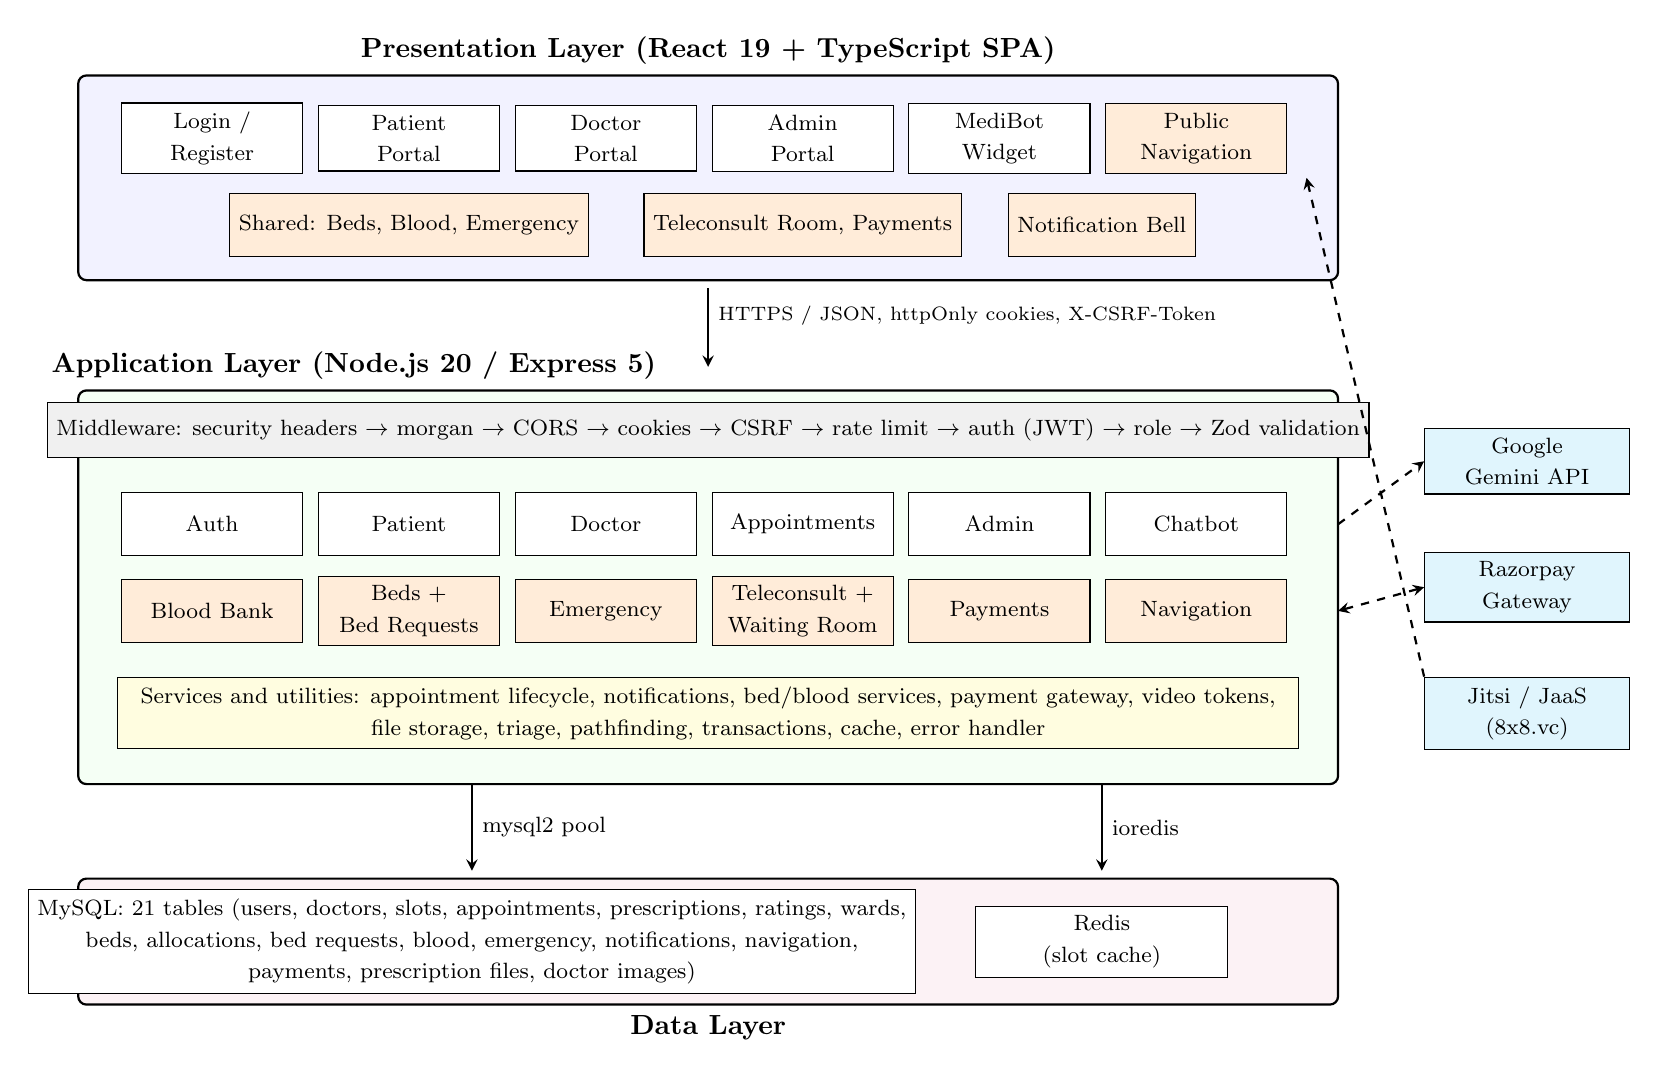
\begin{tikzpicture}[
    font=\footnotesize,
    layer/.style={draw, rectangle, thick, rounded corners=3pt, minimum width=16cm},
    component/.style={draw, rectangle, minimum width=2.3cm, minimum height=0.8cm, align=center, fill=white},
    newc/.style={component, fill=orange!15},
    ext/.style={draw, rectangle, minimum width=2.6cm, minimum height=0.8cm, align=center, fill=cyan!12},
    arrow/.style={->, thick, >=stealth}
]
% Presentation
\node[layer, minimum height=2.6cm, fill=blue!5, label={[font=\bfseries]above:Presentation Layer (React 19 + TypeScript SPA)}] at (0,0) {};
\node[component] at (-6.3,0.5) {Login /\\Register};
\node[component] at (-3.8,0.5) {Patient\\Portal};
\node[component] at (-1.3,0.5) {Doctor\\Portal};
\node[component] at (1.2,0.5) {Admin\\Portal};
\node[component] at (3.7,0.5) {MediBot\\Widget};
\node[newc] at (6.2,0.5) {Public\\Navigation};
\node[newc] at (-3.8,-0.6) {Shared: Beds, Blood, Emergency};
\node[newc] at (1.2,-0.6) {Teleconsult Room, Payments};
\node[newc] at (5.0,-0.6) {Notification Bell};

\draw[arrow] (0,-1.4) -- (0,-2.4) node[pos=0.35, right, font=\scriptsize] {HTTPS / JSON, httpOnly cookies, X-CSRF-Token};

% Application
\node[layer, minimum height=5.0cm, fill=green!4, label={[font=\bfseries, xshift=-4.5cm]above:Application Layer (Node.js 20 / Express 5)}] at (0,-5.2) {};
\node[draw, rectangle, minimum width=15cm, minimum height=0.7cm, fill=gray!12] at (0,-3.2)
{Middleware: security headers $\rightarrow$ morgan $\rightarrow$ CORS $\rightarrow$ cookies $\rightarrow$ CSRF $\rightarrow$ rate limit $\rightarrow$ auth (JWT) $\rightarrow$ role $\rightarrow$ Zod validation};
\node[component] at (-6.3,-4.4) {Auth};
\node[component] at (-3.8,-4.4) {Patient};
\node[component] at (-1.3,-4.4) {Doctor};
\node[component] at (1.2,-4.4) {Appointments};
\node[component] at (3.7,-4.4) {Admin};
\node[component] at (6.2,-4.4) {Chatbot};
\node[newc] at (-6.3,-5.5) {Blood Bank};
\node[newc] at (-3.8,-5.5) {Beds +\\Bed Requests};
\node[newc] at (-1.3,-5.5) {Emergency};
\node[newc] at (1.2,-5.5) {Teleconsult +\\Waiting Room};
\node[newc] at (3.7,-5.5) {Payments};
\node[newc] at (6.2,-5.5) {Navigation};
\node[draw, rectangle, minimum width=15cm, minimum height=0.7cm, fill=yellow!12, align=center] at (0,-6.8)
{Services and utilities: appointment lifecycle, notifications, bed/blood services, payment gateway, video tokens,\\ file storage, triage, pathfinding, transactions, cache, error handler};

\draw[arrow] (-3,-7.7) -- (-3,-8.8) node[midway, right] {mysql2 pool};
\draw[arrow] (5,-7.7) -- (5,-8.8) node[midway, right] {ioredis};

% Data
\node[layer, minimum height=1.6cm, fill=purple!5, label={[font=\bfseries]below:Data Layer}] at (0,-9.7) {};
\node[draw, rectangle, minimum width=9.5cm, minimum height=0.9cm, fill=white, align=center] at (-3,-9.7) {MySQL: 21 tables (users, doctors, slots, appointments, prescriptions, ratings, wards,\\ beds, allocations, bed requests, blood, emergency, notifications, navigation,\\ payments, prescription files, doctor images)};
\node[draw, rectangle, minimum width=3.2cm, minimum height=0.9cm, fill=white, align=center] at (5,-9.7) {Redis\\(slot cache)};

% External
\node[ext] (gem) at (10.4,-3.6) {Google\\Gemini API};
\node[ext] (rzp) at (10.4,-5.2) {Razorpay\\Gateway};
\node[ext] (jit) at (10.4,-6.8) {Jitsi / JaaS\\(8x8.vc)};
\draw[arrow, dashed] (8.0,-4.4) -- (gem.west);
\draw[arrow, dashed, <->] (8.0,-5.5) -- (rzp.west);
\draw[arrow, dashed] (jit.north west) -- (7.6,0.0);
\end{tikzpicture}%
}
\caption{Three-Tier Architecture of Care \& Cure HMS}
\label{fig:arch_ieee}
\end{figure}

Components shaded orange in Figure~\ref{fig:arch_ieee} were added in the second phase. The video call is loaded by the browser directly from JaaS; the backend only decides whether a user may join, keeps the patient in the waiting room until the doctor admits them, and signs the token that opens the room.

\FloatBarrier
\section{Data Flow Diagrams}

\subsection{Level 0 DFD (Context Diagram)}

The Level 0 DFD, shown in Figure~\ref{fig:dfd0}, depicts the system as a single process interacting with seven external entities: Patient, Doctor, Administrator, Visitor, and three external services (Gemini AI, Razorpay and the JaaS video service).

\begin{figure}[H]
\centering
\resizebox{\textwidth}{!}{%
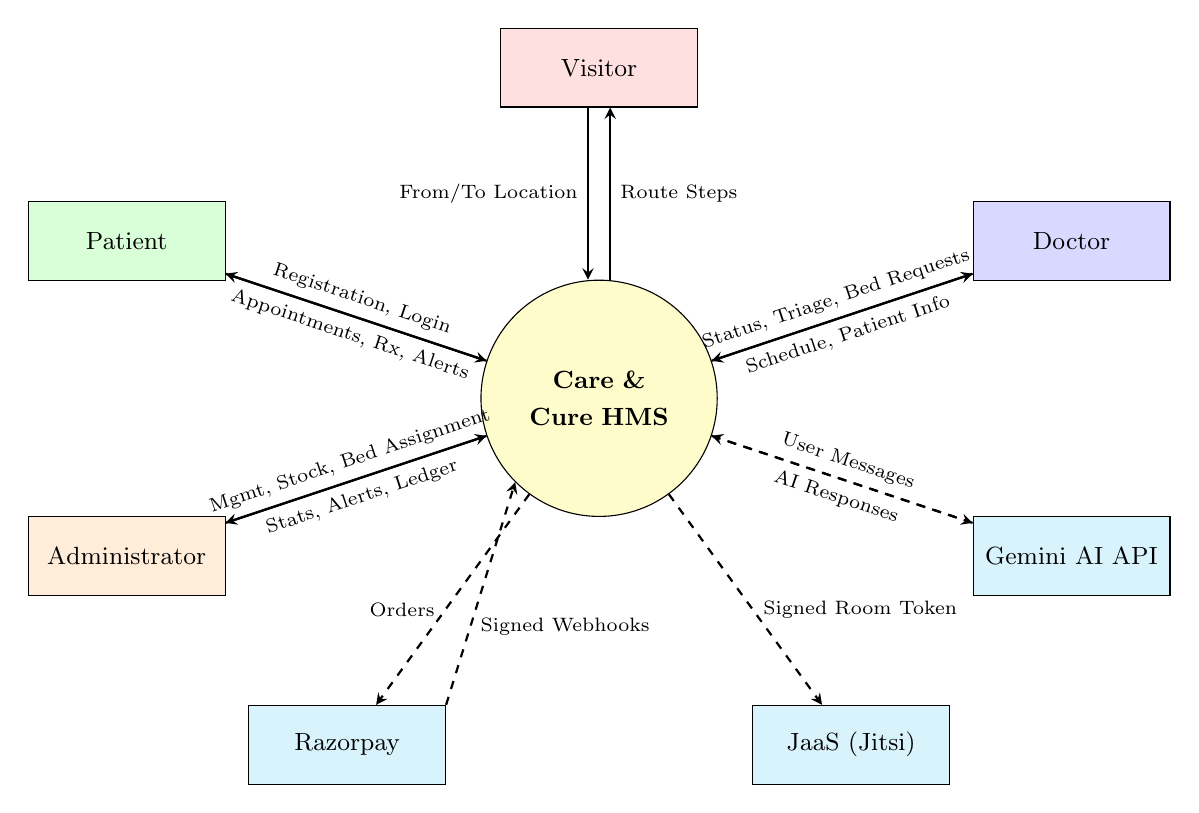
\begin{tikzpicture}[node distance=2cm, font=\small, arrow/.style={thick,->,>=stealth}]

% Central process
\node[draw, circle, fill=yellow!20, minimum size=3cm, text centered, text width=2.5cm] (sys) at (0,0) {\textbf{Care \& Cure HMS}};

% External entities
\node[draw, rectangle, fill=green!15, minimum width=2.5cm, minimum height=1cm, text centered] (pat) at (-6, 2) {Patient};
\node[draw, rectangle, fill=blue!15, minimum width=2.5cm, minimum height=1cm, text centered] (doc) at (6, 2) {Doctor};
\node[draw, rectangle, fill=orange!15, minimum width=2.5cm, minimum height=1cm, text centered] (adm) at (-6, -2) {Administrator};
\node[draw, rectangle, fill=cyan!15, minimum width=2.5cm, minimum height=1cm, text centered] (ai) at (6, -2) {Gemini AI API};

% Patient flows
\draw[arrow] (pat) -- node[above, sloped, font=\scriptsize]{Registration, Login} (sys);
\draw[arrow] (sys) -- node[below, sloped, font=\scriptsize]{Appointments, Rx, Alerts} (pat);

% Doctor flows
\draw[arrow] (doc) -- node[above, sloped, font=\scriptsize]{Status, Triage, Bed Requests} (sys);
\draw[arrow] (sys) -- node[below, sloped, font=\scriptsize]{Schedule, Patient Info} (doc);

% Admin flows
\draw[arrow] (adm) -- node[above, sloped, font=\scriptsize]{Mgmt, Stock, Bed Assignment} (sys);
\draw[arrow] (sys) -- node[below, sloped, font=\scriptsize]{Stats, Alerts, Ledger} (adm);

% AI flows
\draw[arrow, dashed] (sys) -- node[above, sloped, font=\scriptsize]{User Messages} (ai);
\draw[arrow, dashed] (ai) -- node[below, sloped, font=\scriptsize]{AI Responses} (sys);

% Phase-2 entities
\node[draw, rectangle, fill=red!12, minimum width=2.5cm, minimum height=1cm, text centered] (vis) at (0, 4.2) {Visitor};
\node[draw, rectangle, fill=cyan!15, minimum width=2.5cm, minimum height=1cm, text centered] (rzp) at (-3.2, -4.4) {Razorpay};
\node[draw, rectangle, fill=cyan!15, minimum width=2.5cm, minimum height=1cm, text centered] (jit) at (3.2, -4.4) {JaaS (Jitsi)};
\draw[arrow] ([xshift=-4pt]vis.south) -- node[left, font=\scriptsize]{From/To Location} ([xshift=-4pt]sys.north);
\draw[arrow] ([xshift=4pt]sys.north) -- node[right, font=\scriptsize]{Route Steps} ([xshift=4pt]vis.south);
\draw[arrow, dashed] (sys) -- node[left, font=\scriptsize, pos=0.55]{Orders} (rzp);
\draw[arrow, dashed] (rzp.north east) -- node[right, font=\scriptsize, pos=0.35]{Signed Webhooks} (sys.south west);
\draw[arrow, dashed] (sys) -- node[right, font=\scriptsize, pos=0.55]{Signed Room Token} (jit);

\end{tikzpicture}%
}
\caption{Level 0 Data Flow Diagram (Context Diagram)}
\label{fig:dfd0}
\end{figure}

\subsection{Level 1 DFD}

The Level 1 DFD in Figure~\ref{fig:dfd1} decomposes the system into six major processes with their associated data stores and flows.

\begin{figure}[H]
\centering
\resizebox{\textwidth}{!}{%
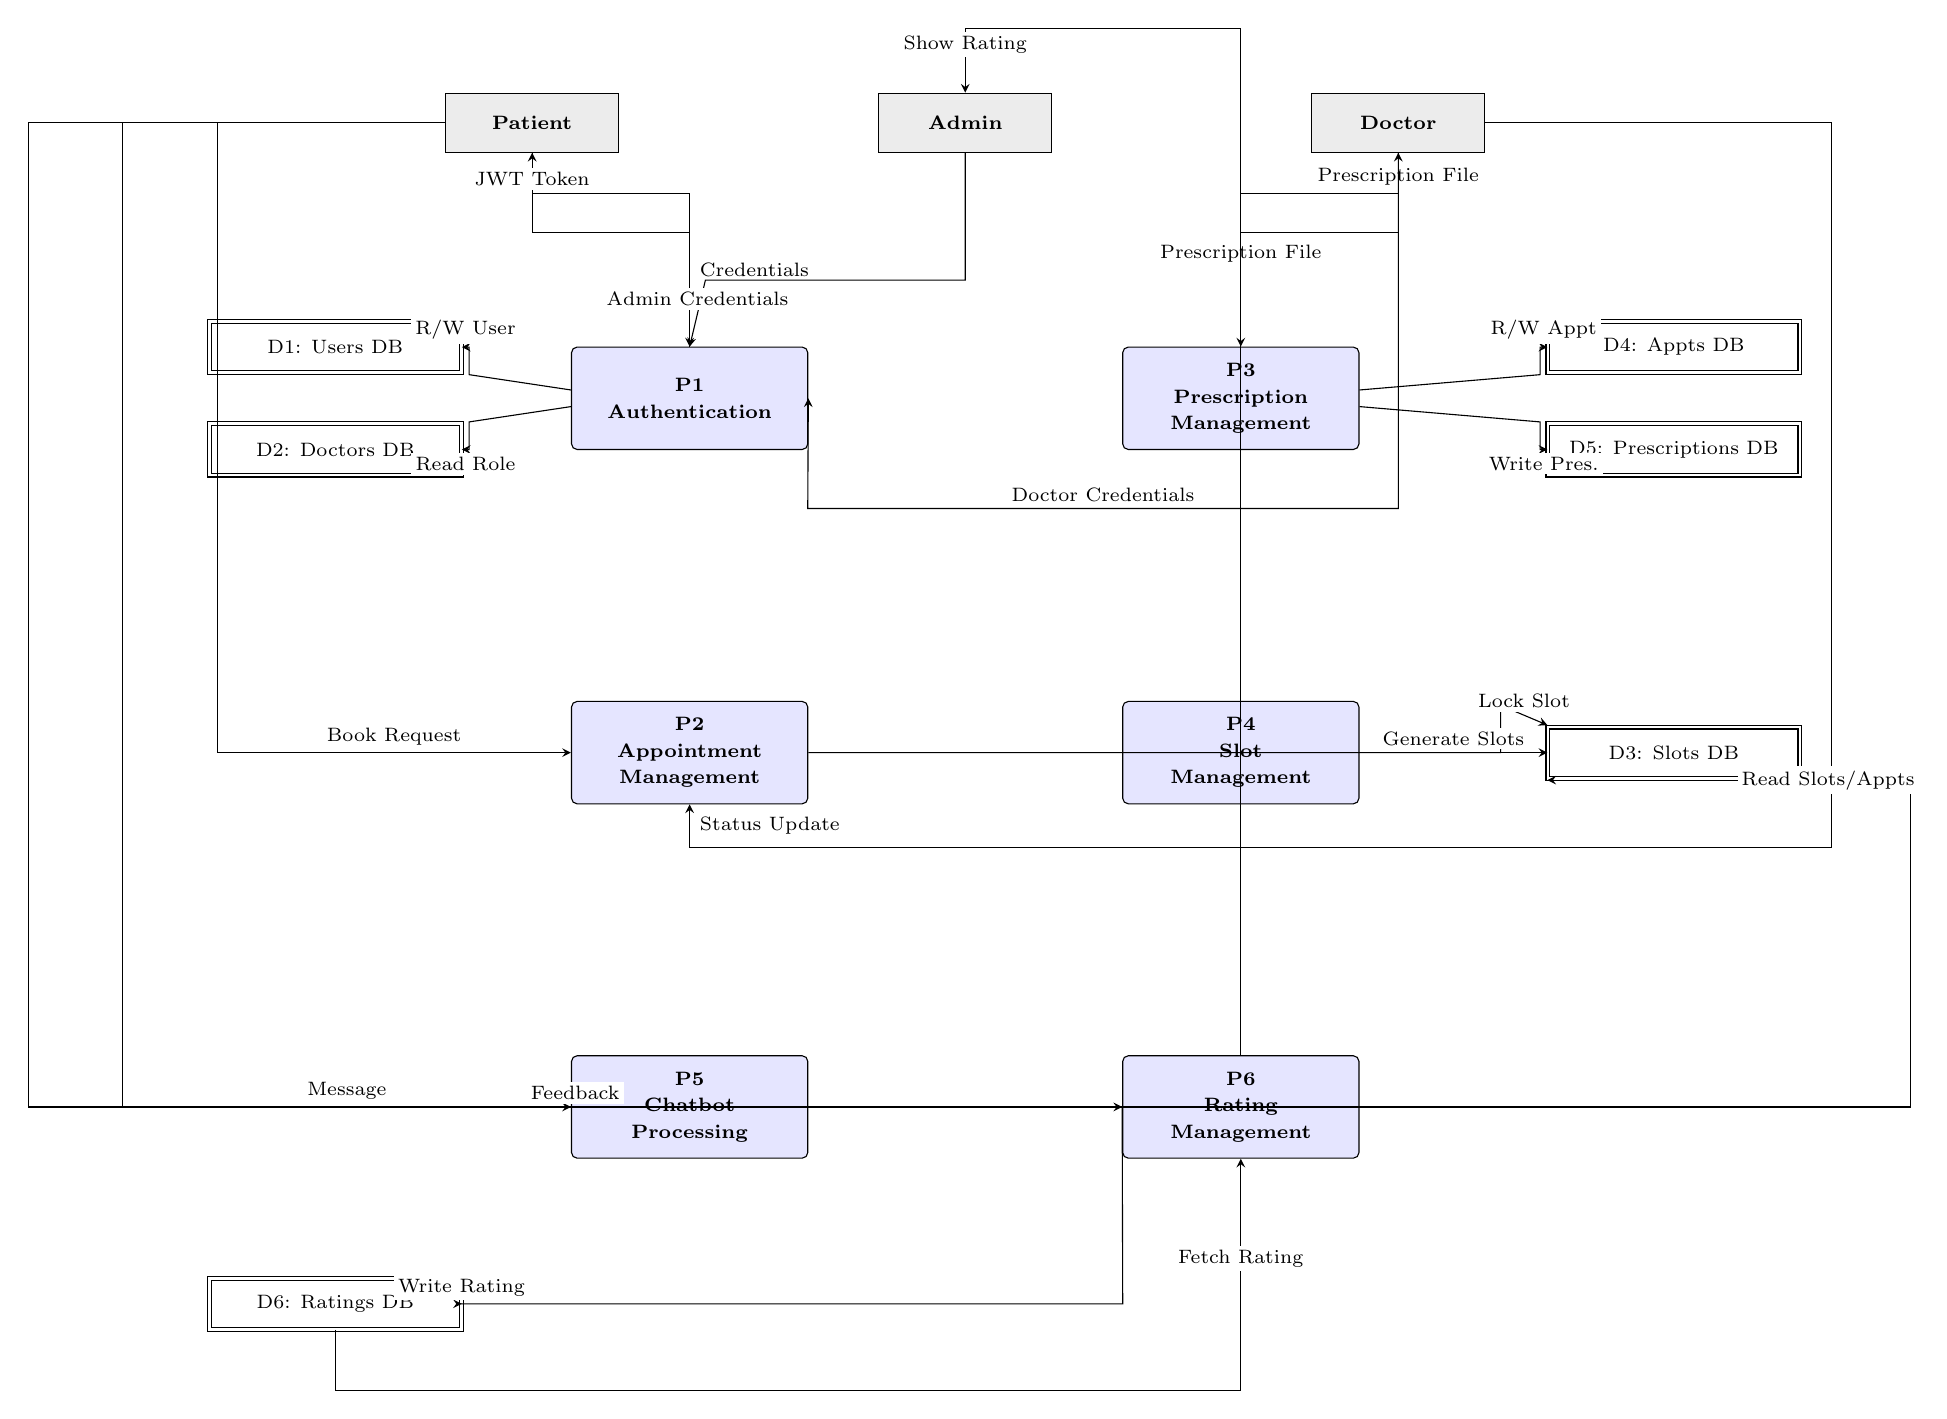
\begin{tikzpicture}[
  process/.style={
    rectangle, draw=black, rounded corners=2pt,
    minimum width=3.0cm, minimum height=1.3cm,
    align=center, fill=blue!10,
    font=\scriptsize\bfseries, inner sep=4pt
  },
  store/.style={
    rectangle, draw=black, double, double distance=1pt,
    minimum width=3.2cm, minimum height=0.65cm,
    align=center, font=\scriptsize, inner sep=3pt
  },
  ext/.style={
    rectangle, draw=black,
    minimum width=2.2cm, minimum height=0.75cm,
    align=center, font=\scriptsize\bfseries, fill=gray!15
  },
  arr/.style={->, >=stealth, thin},
  lbl/.style={font=\scriptsize, inner sep=1.5pt, fill=white}
]
\node[ext] (pat) at ( 3.0, 17.5) {Patient};
\node[ext] (adm) at ( 8.5, 17.5) {Admin};
\node[ext] (doc) at (14.0, 17.5) {Doctor};
\node[process] (p1) at ( 5.0, 14.0) {P1\\Authentication};
\node[process] (p3) at (12.0, 14.0) {P3\\Prescription\\Management};
\node[process] (p2) at ( 5.0,  9.5) {P2\\Appointment\\Management};
\node[process] (p4) at (12.0,  9.5) {P4\\Slot\\Management};
\node[process] (p5) at ( 5.0,  5.0) {P5\\Chatbot\\Processing};
\node[process] (p6) at (12.0,  5.0) {P6\\Rating\\Management};
\node[store] (ds1) at ( 0.5, 14.65) {D1: Users DB};
\node[store] (ds2) at ( 0.5, 13.35) {D2: Doctors DB};
\node[store] (ds6) at ( 0.5,  2.5)  {D6: Ratings DB};
\node[store] (ds4) at (17.5, 14.65) {D4: Appts DB};
\node[store] (ds5) at (17.5, 13.35) {D5: Prescriptions DB};
\node[store] (ds3) at (17.5,  9.5)  {D3: Slots DB};
\draw[arr] (pat.south)--(3.0,16.6)--(5.0,16.6)--node[lbl,right=2pt]{Credentials}(p1.north);
\draw[arr] (p1.north)--(5.0,16.1)--(3.0,16.1)--node[lbl,above=1pt]{JWT Token}(pat.south);
\draw[arr] (adm.south)--(8.5,15.5)--(5.2,15.5)--node[lbl,above=1pt]{Admin Credentials}(p1.north);
\draw[arr] (doc.south)--(14.0,16.6)--(12.0,16.6)--node[lbl,above=1pt]{Prescription File}(p3.north);
\draw[arr] (p3.north)--(12.0,16.1)--(14.0,16.1)--node[lbl,above=1pt]{Prescription File}(doc.south);
\draw[arr] (doc.south)--(14.0,12.6)--node[lbl,above=1pt]{Doctor Credentials}(6.5,12.6)--(p1.east);
\draw[arr] (pat.west)--(-1.0,17.5)--(-1.0,9.5)--node[lbl,above=1pt]{Book Request}(p2.west);
\draw[arr] (pat.west)--(-2.2,17.5)--(-2.2,5.0)--node[lbl,above=1pt]{Message}(p5.west);
\draw[arr] (pat.west)--(-3.4,17.5)--(-3.4,5.0)--node[lbl,above=1pt]{Feedback}(p6.west);
\draw[arr] (doc.east)--(19.5,17.5)--(19.5,8.3)--(5.0,8.3)--node[lbl,right=2pt]{Status Update}(p2.south);
\draw[arr] (p6.north)--(12.0,18.7)--(8.5,18.7)--node[lbl,above=1pt]{Show Rating}(adm.north);
\draw[arr] ([yshift=3pt]p1.west)--(2.2,14.3)--(2.2,14.65)--node[lbl,above=1pt]{R/W User}(ds1.east);
\draw[arr] ([yshift=-3pt]p1.west)--(2.2,13.7)--(2.2,13.35)--node[lbl,below=1pt]{Read Role}(ds2.east);
\draw[arr] ([yshift=3pt]p3.east)--(15.8,14.3)--(15.8,14.65)--node[lbl,above=1pt]{R/W Appt}(ds4.west);
\draw[arr] ([yshift=-3pt]p3.east)--(15.8,13.7)--(15.8,13.35)--node[lbl,below=1pt]{Write Pres.}(ds5.west);
\draw[arr] (p2.east)--(15.3,9.5)--(15.3,10.1)--node[lbl,above=1pt]{Lock Slot}($(ds3.west)+(0,+0.35)$);
\draw[arr] (p4.east)--node[lbl,above=1pt]{Generate Slots}(ds3.west);
\draw[arr] (p5.east)--(20.5,5.0)--(20.5,9.15)--node[lbl,right=3pt]{Read Slots/Appts}($(ds3.west)+(0,-0.35)$);
\draw[arr] (p6.west)--(10.5,2.5)--(2.1,2.5)--node[lbl,pos=0.35,above=1pt]{Write Rating}(ds6.east);
\draw[arr] (ds6.south)--(0.5,1.4)--(12.0,1.4)--node[lbl,above=1pt]{Fetch Rating}(p6.south);
\end{tikzpicture}%
}
\caption{Level-1 Data Flow Diagram}
\label{fig:dfd1}
\end{figure}

\subsection{Level 1 DFD for the Enhanced Modules}

Figure~\ref{fig:dfd1b} decomposes the processes added in this phase. Doctors send bed and discharge requests to P8, which the administrator fulfils, and the emergency process P9 raises its admissions as emergency bed requests. Every process that changes clinical state also writes to the notifications store (D13), which is read by the notification bell of each user.

\begin{figure}[H]
\centering
\resizebox{\textwidth}{!}{%
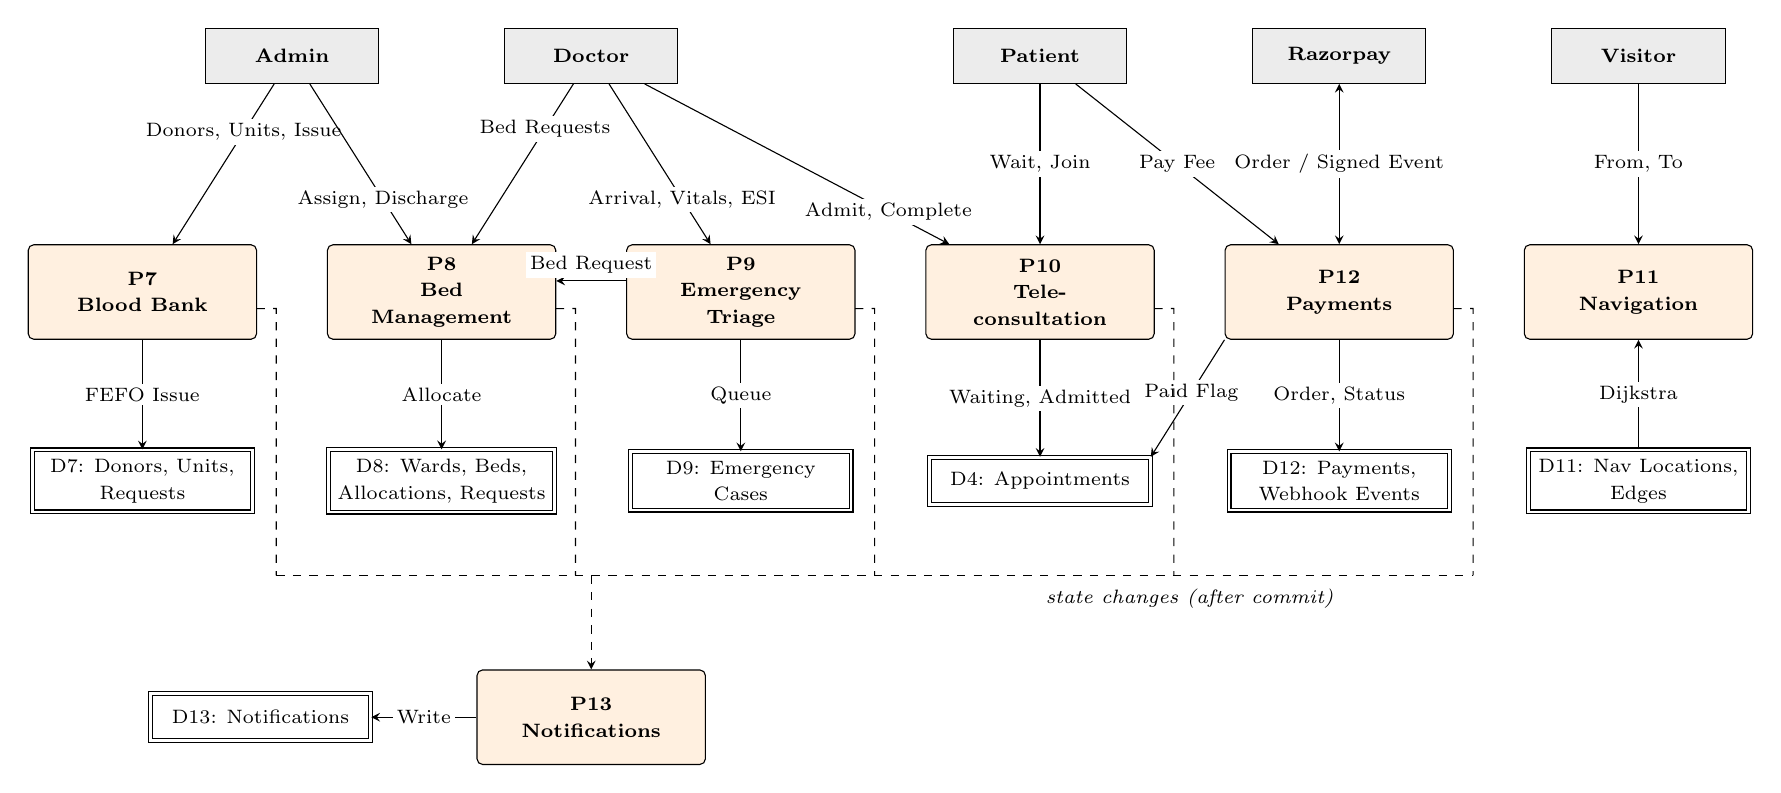
\begin{tikzpicture}[
  process/.style={rectangle, draw=black, rounded corners=2pt, minimum width=2.9cm, minimum height=1.2cm, align=center, fill=orange!12, font=\scriptsize\bfseries},
  store/.style={rectangle, draw=black, double, double distance=1pt, minimum width=2.8cm, minimum height=0.6cm, align=center, font=\scriptsize},
  ext/.style={rectangle, draw=black, minimum width=2.2cm, minimum height=0.7cm, align=center, font=\scriptsize\bfseries, fill=gray!15},
  arr/.style={->, >=stealth, thin},
  bus/.style={dashed, thin},
  lbl/.style={font=\scriptsize, inner sep=1.5pt, fill=white}
]
% externals
\node[ext] (adm) at (1.9,9) {Admin};
\node[ext] (doc) at (5.7,9) {Doctor};
\node[ext] (pat) at (11.4,9) {Patient};
\node[ext] (rzp) at (15.2,9) {Razorpay};
\node[ext] (vis) at (19,9) {Visitor};
% processes
\node[process] (p7)  at (0,6)    {P7\\Blood Bank};
\node[process] (p8)  at (3.8,6)  {P8\\Bed\\Management};
\node[process] (p9)  at (7.6,6)  {P9\\Emergency\\Triage};
\node[process] (p10) at (11.4,6) {P10\\Tele-\\consultation};
\node[process] (p12) at (15.2,6) {P12\\Payments};
\node[process] (p11) at (19,6)   {P11\\Navigation};
% stores
\node[store] (d7)  at (0,3.6)    {D7: Donors, Units,\\Requests};
\node[store] (d8)  at (3.8,3.6)  {D8: Wards, Beds,\\Allocations, Requests};
\node[store] (d9)  at (7.6,3.6)  {D9: Emergency\\Cases};
\node[store] (d4)  at (11.4,3.6) {D4: Appointments};
\node[store] (d12) at (15.2,3.6) {D12: Payments,\\Webhook Events};
\node[store] (d11) at (19,3.6)   {D11: Nav Locations,\\Edges};
\node[process] (p13) at (5.7,0.6) {P13\\Notifications};
\node[store] (d13) at (1.5,0.6) {D13: Notifications};
% external -> process
\draw[arr] (adm) -- node[lbl, pos=0.3]{Donors, Units, Issue} (p7);
\draw[arr] (adm) -- node[lbl, pos=0.72]{Assign, Discharge} (p8);
\draw[arr] (doc) -- node[lbl, pos=0.28]{Bed Requests} (p8);
\draw[arr] (doc) -- node[lbl, pos=0.72]{Arrival, Vitals, ESI} (p9);
\draw[arr] (doc) -- node[lbl, pos=0.8]{Admit, Complete} (p10);
\draw[arr] (pat) -- node[lbl]{Wait, Join} (p10);
\draw[arr] (pat) -- node[lbl, pos=0.5]{Pay Fee} (p12);
\draw[arr, <->] (rzp) -- node[lbl]{Order / Signed Event} (p12);
\draw[arr] (vis) -- node[lbl]{From, To} (p11);
% process -> store
\draw[arr] (p7) -- node[lbl]{FEFO Issue} (d7);
\draw[arr] (p8) -- node[lbl]{Allocate} (d8);
\draw[arr] (p9) -- node[lbl]{Queue} (d9);
\draw[arr] (p10) -- node[lbl]{Waiting, Admitted} (d4);
\draw[arr] (p12) -- node[lbl]{Order, Status} (d12);
\draw[arr] (p12.south west) -- node[lbl, pos=0.45]{Paid Flag} (d4.north east);
\draw[arr] (d11) -- node[lbl]{Dijkstra} (p11);
\draw[arr] ([yshift=4pt]p9.west) -- node[lbl, above=1pt]{Bed Request} ([yshift=4pt]p8.east);
% notification bus
\foreach \x in {0,3.8,7.6,11.4,15.2} {
  \draw[bus] ([yshift=-6pt]\x+1.45,6) -- (\x+1.7,5.79) -- (\x+1.7,2.4);
}
\draw[bus] (1.7,2.4) -- (16.9,2.4);
\node[lbl, font=\scriptsize\itshape] at (13.3,2.1) {state changes (after commit)};
\draw[arr, dashed] (5.7,2.4) -- (p13.north);
\draw[arr] (p13) -- node[lbl]{Write} (d13);
\end{tikzpicture}%
}
\caption{Level-1 Data Flow Diagram of the Enhanced Modules}
\label{fig:dfd1b}
\end{figure}

\FloatBarrier
\section{Database Design}

\subsection{Entity-Relationship Diagram}

The core database comprises six entities with the following relationships and cardinalities. The fifteen tables added in this phase are shown separately in Section~\ref{sec:er-ext}.

\begin{figure}[h]
\centering
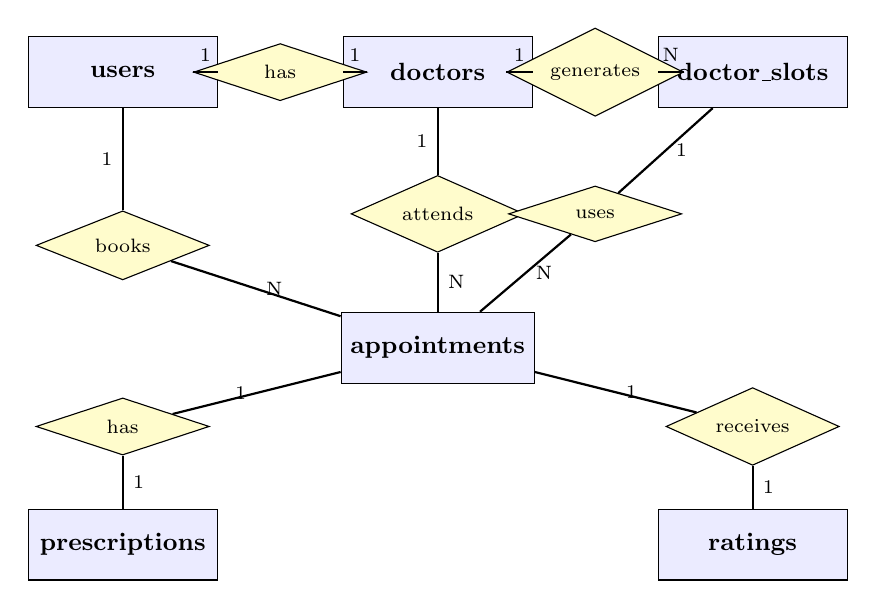
\begin{tikzpicture}[
  ent/.style={rectangle, draw=black, minimum width=2.4cm, minimum height=0.9cm,
              align=center, font=\small\bfseries, fill=blue!8},
  rel/.style={diamond, draw=black, aspect=2, minimum width=2.2cm,
              minimum height=0.7cm, align=center, font=\scriptsize, fill=yellow!20},
  att/.style={ellipse, draw=black, minimum width=1.8cm, minimum height=0.55cm,
              align=center, font=\scriptsize},
  pk/.style={ellipse, draw=black, minimum width=1.8cm, minimum height=0.55cm,
             align=center, font=\scriptsize\underbar, text=black},
  lin/.style={-, thick},
  arr/.style={->, >=stealth, thick}
]
  % Entities
  \node[ent] (users)   at (0,   0)    {users};
  \node[ent] (doctors) at (4,   0)    {doctors};
  \node[ent] (slots)   at (8,   0)    {doctor\_slots};
  \node[ent] (appts)   at (4,  -3.5)  {appointments};
  \node[ent] (pres)    at (0,  -6)    {prescriptions};
  \node[ent] (ratings) at (8,  -6)    {ratings};

  % Relationships
  \node[rel] (r1) at (2,  0)    {has};
  \node[rel] (r2) at (6,  0)    {generates};
  \node[rel] (r3) at (0, -2.2)  {books};
  \node[rel] (r4) at (4, -1.8)  {attends};
  \node[rel] (r5) at (6, -1.8)  {uses};
  \node[rel] (r6) at (0, -4.5)  {has};
  \node[rel] (r7) at (8, -4.5)  {receives};

  % users -- has -- doctors  (1:1 for doctor role)
  \draw[lin] (users)   -- node[above]{\scriptsize 1} (r1);
  \draw[lin] (r1)      -- node[above]{\scriptsize 1} (doctors);

  % doctors -- generates -- slots  (1:N)
  \draw[lin] (doctors) -- node[above]{\scriptsize 1} (r2);
  \draw[lin] (r2)      -- node[above]{\scriptsize N} (slots);

  % users(patient) -- books -- appointments  (1:N)
  \draw[lin] (users)   -- node[left]{\scriptsize 1} (r3);
  \draw[lin] (r3)      -- node[right]{\scriptsize N} (appts);

  % doctors -- attends -- appointments  (1:N)
  \draw[lin] (doctors) -- node[left]{\scriptsize 1} (r4);
  \draw[lin] (r4)      -- node[right]{\scriptsize N} (appts);

  % slots -- uses -- appointments  (1:N over time, at most one active)
  \draw[lin] (slots)   -- node[right]{\scriptsize 1} (r5);
  \draw[lin] (r5)      -- node[right]{\scriptsize N} (appts);

  % appointments -- has -- prescriptions  (1:1)
  \draw[lin] (appts)   -- node[left]{\scriptsize 1} (r6);
  \draw[lin] (r6)      -- node[right]{\scriptsize 1} (pres);

  % appointments -- receives -- ratings  (1:1)
  \draw[lin] (appts)   -- node[right]{\scriptsize 1} (r7);
  \draw[lin] (r7)      -- node[right]{\scriptsize 1} (ratings);
\end{tikzpicture}
\caption{Entity-Relationship Diagram of Care \& Cure HMS}
\label{figure:er}
\end{figure}

\subsection{Database Schema}

The following tables specify the full schema for each database entity.

\begin{longtable}{|L{2.8cm}|L{2.6cm}|L{2.2cm}|L{5.2cm}|}
\caption{Schema: \texttt{users} table} \label{tab:users} \\
\hline
\textbf{Column} & \textbf{Type} & \textbf{Constraints} & \textbf{Description} \\
\hline
\endfirsthead
\hline
\textbf{Column} & \textbf{Type} & \textbf{Constraints} & \textbf{Description} \\
\hline
\endhead
\hline
\endfoot
id             & INT              & PK, AUTO\_INC   & Surrogate primary key \\
\hline
name           & VARCHAR(100)     & NOT NULL        & Full name of the user \\
\hline
guardian\_name & VARCHAR(150)     & NULL            & Guardian/relative name \\
\hline
gender         & ENUM             & NULL            & 'male', 'female', 'other' \\
\hline
age            & INT              & NULL            & Age in years \\
\hline
weight         & DECIMAL(5,2)     & NULL            & Body weight in kilograms \\
\hline
medical\_history & TEXT           & NULL            & Free-text prior conditions \\
\hline
phone          & VARCHAR(20)      & NULL            & Contact number \\
\hline
email          & VARCHAR(150)     & UNIQUE NOT NULL & Login identifier \\
\hline
password       & VARCHAR(255)     & NOT NULL        & bcrypt-hashed credential \\
\hline
address        & TEXT             & NULL            & Street address \\
\hline
city           & VARCHAR(100)     & NULL            & City of residence \\
\hline
role           & ENUM             & NOT NULL        & 'patient','doctor','admin' \\
\hline
created\_at    & TIMESTAMP        & DEFAULT NOW()   & Account creation time \\
\hline
\end{longtable}

\begin{longtable}{|L{2.8cm}|L{2.6cm}|L{2.2cm}|L{5.2cm}|}
\caption{Schema: \texttt{doctors} table} \label{tab:doctors} \\
\hline
\textbf{Column} & \textbf{Type} & \textbf{Constraints} & \textbf{Description} \\
\hline
\endfirsthead
\hline
\textbf{Column} & \textbf{Type} & \textbf{Constraints} & \textbf{Description} \\
\hline
\endhead
\hline
\endfoot
id             & INT              & PK, AUTO\_INC   & Doctor-specific key \\
\hline
user\_id       & INT              & FK $\rightarrow$ users(id), UNIQUE, CASCADE & Maps to users table (1-to-1) \\
\hline
specialization & VARCHAR(100)     & NOT NULL        & Medical specialty \\
\hline
fees           & DECIMAL(10,2)    & NOT NULL, DEFAULT 0 & Consultation fee (INR) \\
\hline
rating         & DECIMAL(3,2)     & NOT NULL, DEFAULT 0 & average rating \\
\hline
rating\_count  & INT              & NOT NULL, DEFAULT 0 & Total ratings received \\
\hline
profile\_image & VARCHAR(255)     & NULL            & Version token for the photo URL; bytes in \texttt{doctor\_images} (v2) \\
\hline
\end{longtable}

\begin{longtable}{|L{2.8cm}|L{2.6cm}|L{2.2cm}|L{5.2cm}|}
\caption{Schema: \texttt{doctor\_slots} table} \label{tab:slots} \\
\hline
\textbf{Column} & \textbf{Type} & \textbf{Constraints} & \textbf{Description} \\
\hline
\endfirsthead
\hline
\textbf{Column} & \textbf{Type} & \textbf{Constraints} & \textbf{Description} \\
\hline
\endhead
\hline
\endfoot
id          & INT           & PK, AUTO\_INC     &  primary key \\
\hline
doctor\_id  & INT           & FK $\rightarrow$ doctors(id), CASCADE & Owning doctor \\
\hline
date        & DATE          & NOT NULL          & Calendar date of slot \\
\hline
time        & TIME          & NOT NULL          & Start time (HH:MM:SS) \\
\hline
is\_booked  & TINYINT(1)    & NOT NULL, DEFAULT 0 & 1 if slot is confirmed booked \\
\hline
is\_available & TINYINT(1)  & NOT NULL, DEFAULT 1 & 0 if admin has blocked slot \\
\hline
-- UNIQUE   & (doctor\_id, date, time) & UNIQUE KEY & Prevents duplicate slot rows \\
\hline
\end{longtable}

\begin{longtable}{|L{2.8cm}|L{2.6cm}|L{2.2cm}|L{5.2cm}|}
\caption{Schema: \texttt{appointments} table} \label{tab:appts} \\
\hline
\textbf{Column} & \textbf{Type} & \textbf{Constraints} & \textbf{Description} \\
\hline
\endfirsthead
\hline
\textbf{Column} & \textbf{Type} & \textbf{Constraints} & \textbf{Description} \\
\hline
\endhead
\hline
\endfoot
id          & INT           & PK, AUTO\_INC     &  primary key \\
\hline
patient\_id & INT           & FK $\rightarrow$ users(id)    & Booking patient \\
\hline
doctor\_id  & INT           & FK $\rightarrow$ doctors(id)  & Assigned doctor \\
\hline
slot\_id    & INT           & FK $\rightarrow$ doctor\_slots(id), INDEX & Slot booked (kept after cancellation) \\
\hline
active\_slot\_id & INT     & UNIQUE, NULL      & Equals slot\_id while the visit is live, NULL once cancelled; prevents double-booking (v2) \\
\hline
status      & ENUM          & DEFAULT 'pending' & 'pending','completed','cancelled' \\
\hline
reason      & VARCHAR(255)  & NULL              & Patient-stated reason for visit \\
\hline
consultation\_type & ENUM & DEFAULT 'in\_person' & 'in\_person' or 'video' (v2) \\
\hline
video\_room  & VARCHAR(64)   & UNIQUE, NULL      & Random room name for video visits (v2) \\
\hline
payment\_status & ENUM       & DEFAULT 'unpaid'  & 'unpaid' or 'paid' (v2) \\
\hline
video\_waiting\_at & DATETIME & NULL            & Patient's last poll from the waiting room (v2) \\
\hline
video\_admitted\_at & DATETIME & NULL           & When the doctor admitted the patient (v2) \\
\hline
created\_at & TIMESTAMP     & DEFAULT NOW()     & Booking creation timestamp \\
\hline
\end{longtable}

\begin{longtable}{|L{2.8cm}|L{2.6cm}|L{2.2cm}|L{5.2cm}|}
\caption{Schema: \texttt{prescriptions} table} \label{tab:pres} \\
\hline
\textbf{Column} & \textbf{Type} & \textbf{Constraints} & \textbf{Description} \\
\hline
\endfirsthead
\hline
\textbf{Column} & \textbf{Type} & \textbf{Constraints} & \textbf{Description} \\
\hline
\endhead
\hline
\endfoot
id              & INT           & PK, AUTO\_INC    &  primary key \\
\hline
appointment\_id & INT           & FK $\rightarrow$ appointments(id), UNIQUE & 1 prescription per appointment \\
\hline
doctor\_id      & INT           & FK $\rightarrow$ doctors(id) & Prescribing doctor \\
\hline
patient\_id     & INT           & FK $\rightarrow$ users(id)   & Receiving patient \\
\hline
notes           & TEXT          & NULL             & Doctor's free-text clinical notes \\
\hline
file\_url       & VARCHAR(500)  & NULL             & Access-checked file URL \texttt{/api/\allowbreak files/\allowbreak prescriptions/:id}; bytes in \texttt{prescription\_files} (v2) \\
\hline
created\_at     & TIMESTAMP     & DEFAULT NOW()    & Prescription creation timestamp \\
\hline
\end{longtable}

\begin{longtable}{|L{2.8cm}|L{2.6cm}|L{2.2cm}|L{5.2cm}|}
\caption{Schema: \texttt{ratings} table} \label{tab:ratings} \\
\hline
\textbf{Column} & \textbf{Type} & \textbf{Constraints} & \textbf{Description} \\
\hline
\endfirsthead
\hline
\textbf{Column} & \textbf{Type} & \textbf{Constraints} & \textbf{Description} \\
\hline
\endhead
\hline
\endfoot
id              & INT          & PK, AUTO\_INC   &  primary key \\
\hline
appointment\_id & INT          & FK $\rightarrow$ appointments(id), UNIQUE & One rating per appointment \\
\hline
doctor\_id      & INT          & FK $\rightarrow$ doctors(id) & Rated doctor \\
\hline
patient\_id     & INT          & FK $\rightarrow$ users(id)   & Rating patient \\
\hline
stars           & TINYINT      & CHECK (1--5)     & Integer star score \\
\hline
created\_at     & TIMESTAMP    & DEFAULT NOW()    & Rating submission timestamp \\
\hline
\end{longtable}

The tables added in the second phase are specified below. Columns marked (v2) in the tables above were added to existing tables by migrations.

\begin{longtable}{|L{3.3cm}|L{2.5cm}|L{2.4cm}|L{4.6cm}|}
\caption{Schema: \texttt{wards} table} \label{tab:wards} \\
\hline
\textbf{Column} & \textbf{Type} & \textbf{Constraints} & \textbf{Description} \\
\hline
\endfirsthead
\hline
\textbf{Column} & \textbf{Type} & \textbf{Constraints} & \textbf{Description} \\
\hline
\endhead
\hline
\endfoot
id & INT & PK, AUTO\_INC & Primary key \\
\hline
name & VARCHAR(100) & UNIQUE NOT NULL & Ward name \\
\hline
ward\_type & ENUM & NOT NULL & general, icu, emergency, maternity, pediatric, private \\
\hline
floor & INT & DEFAULT 0 & Floor number \\
\hline
created\_at & TIMESTAMP & DEFAULT NOW() & Creation time \\
\hline
\end{longtable}
\begin{longtable}{|L{3.3cm}|L{2.5cm}|L{2.4cm}|L{4.6cm}|}
\caption{Schema: \texttt{beds} table} \label{tab:beds} \\
\hline
\textbf{Column} & \textbf{Type} & \textbf{Constraints} & \textbf{Description} \\
\hline
\endfirsthead
\hline
\textbf{Column} & \textbf{Type} & \textbf{Constraints} & \textbf{Description} \\
\hline
\endhead
\hline
\endfoot
id & INT & PK, AUTO\_INC & Primary key \\
\hline
ward\_id & INT & FK $\rightarrow$ wards(id), CASCADE & Owning ward \\
\hline
bed\_number & VARCHAR(20) & NOT NULL & Label such as ICU-03 \\
\hline
status & ENUM & DEFAULT 'available' & available, occupied, maintenance, reserved \\
\hline
daily\_rate & DECIMAL(10,2) & DEFAULT 0 & Charge per day (INR) \\
\hline
-- UNIQUE & (ward\_id, bed\_number) & UNIQUE KEY & No duplicate labels in a ward \\
\hline
\end{longtable}
\begin{longtable}{|L{3.3cm}|L{2.5cm}|L{2.4cm}|L{4.6cm}|}
\caption{Schema: \texttt{bed\_allocations} table} \label{tab:allocs} \\
\hline
\textbf{Column} & \textbf{Type} & \textbf{Constraints} & \textbf{Description} \\
\hline
\endfirsthead
\hline
\textbf{Column} & \textbf{Type} & \textbf{Constraints} & \textbf{Description} \\
\hline
\endhead
\hline
\endfoot
id & INT & PK, AUTO\_INC & Primary key \\
\hline
bed\_id & INT & FK $\rightarrow$ beds(id) & Allocated bed \\
\hline
patient\_id & INT & FK $\rightarrow$ users(id), CASCADE & Admitted patient \\
\hline
allocated\_by & INT & FK $\rightarrow$ users(id), SET NULL & Administrator who assigned the bed \\
\hline
attending\_doctor\_id & INT & FK $\rightarrow$ users(id), SET NULL & Doctor whose request led to the stay; sees it and may request discharge \\
\hline
reason & VARCHAR(255) & NULL & Reason for admission \\
\hline
admitted\_at & DATETIME & DEFAULT NOW() & Admission time \\
\hline
discharged\_at & DATETIME & NULL & NULL while the stay is open \\
\hline
open\_patient\_id & INT & UNIQUE, NULL & Equals patient\_id while open, NULL after discharge \\
\hline
open\_bed\_id & INT & UNIQUE, NULL & Equals bed\_id while open, NULL after discharge \\
\hline
\end{longtable}
\begin{longtable}{|L{3.3cm}|L{2.5cm}|L{2.4cm}|L{4.6cm}|}
\caption{Schema: \texttt{blood\_donors} table} \label{tab:donors} \\
\hline
\textbf{Column} & \textbf{Type} & \textbf{Constraints} & \textbf{Description} \\
\hline
\endfirsthead
\hline
\textbf{Column} & \textbf{Type} & \textbf{Constraints} & \textbf{Description} \\
\hline
\endhead
\hline
\endfoot
id & INT & PK, AUTO\_INC & Primary key \\
\hline
name & VARCHAR(100) & NOT NULL & Donor name \\
\hline
blood\_group & ENUM & NOT NULL, INDEX & A+, A$-$, B+, B$-$, AB+, AB$-$, O+, O$-$ \\
\hline
phone / email & VARCHAR & phone NOT NULL & Contact details \\
\hline
last\_donation\_date & DATE & NULL & Used to enforce the 56-day interval \\
\hline
\end{longtable}
\begin{longtable}{|L{3.3cm}|L{2.5cm}|L{2.4cm}|L{4.6cm}|}
\caption{Schema: \texttt{blood\_units} table} \label{tab:units} \\
\hline
\textbf{Column} & \textbf{Type} & \textbf{Constraints} & \textbf{Description} \\
\hline
\endfirsthead
\hline
\textbf{Column} & \textbf{Type} & \textbf{Constraints} & \textbf{Description} \\
\hline
\endhead
\hline
\endfoot
id & INT & PK, AUTO\_INC & Primary key \\
\hline
donor\_id & INT & FK $\rightarrow$ blood\_donors, SET NULL & Source donor \\
\hline
blood\_group & ENUM & NOT NULL & Group of the unit \\
\hline
component & ENUM & NOT NULL & whole\_blood, packed\_rbc, plasma, platelets \\
\hline
volume\_ml & INT & NOT NULL & Volume in millilitres \\
\hline
collected\_on / expires\_on & DATE & NOT NULL & Expiry computed from component shelf life \\
\hline
status & ENUM & DEFAULT 'available' & available, issued, expired, discarded \\
\hline
request\_id & INT & FK $\rightarrow$ blood\_requests, SET NULL & Request the unit was issued to \\
\hline
-- INDEX & (status, component, blood\_group, expires\_on) & INDEX & Serves the FEFO stock query \\
\hline
\end{longtable}
\begin{longtable}{|L{3.3cm}|L{2.5cm}|L{2.4cm}|L{4.6cm}|}
\caption{Schema: \texttt{blood\_requests} table} \label{tab:bloodreq} \\
\hline
\textbf{Column} & \textbf{Type} & \textbf{Constraints} & \textbf{Description} \\
\hline
\endfirsthead
\hline
\textbf{Column} & \textbf{Type} & \textbf{Constraints} & \textbf{Description} \\
\hline
\endhead
\hline
\endfoot
id & INT & PK, AUTO\_INC & Primary key \\
\hline
patient\_id & INT & FK $\rightarrow$ users(id), CASCADE & Recipient \\
\hline
requested\_by & INT & FK $\rightarrow$ users(id), SET NULL & Requesting doctor or admin \\
\hline
blood\_group, component & ENUM & NOT NULL & What is needed \\
\hline
units\_requested & INT & NOT NULL & Number of units \\
\hline
urgency & ENUM & DEFAULT 'routine' & routine, urgent, emergency \\
\hline
status & ENUM & DEFAULT 'pending' & pending, fulfilled, rejected, cancelled \\
\hline
notes & VARCHAR(500) & NULL & Rejection or clinical note \\
\hline
fulfilled\_at & DATETIME & NULL & Time of issue \\
\hline
\end{longtable}
\begin{longtable}{|L{3.3cm}|L{2.5cm}|L{2.4cm}|L{4.6cm}|}
\caption{Schema: \texttt{emergency\_cases} table} \label{tab:ercases} \\
\hline
\textbf{Column} & \textbf{Type} & \textbf{Constraints} & \textbf{Description} \\
\hline
\endfirsthead
\hline
\textbf{Column} & \textbf{Type} & \textbf{Constraints} & \textbf{Description} \\
\hline
\endhead
\hline
\endfoot
id & INT & PK, AUTO\_INC & Primary key \\
\hline
patient\_id & INT & FK $\rightarrow$ users(id), SET NULL & Linked registered patient, if any \\
\hline
patient\_name, age, gender, contact\_phone & mixed & name NOT NULL & Details captured at the door \\
\hline
chief\_complaint & VARCHAR(500) & NOT NULL & Presenting complaint \\
\hline
arrival\_mode & ENUM & DEFAULT 'walk\_in' & walk\_in, ambulance, referral \\
\hline
triage\_level & TINYINT & NOT NULL & ESI level 1 (most urgent) to 5 \\
\hline
heart\_rate, resp\_rate, bp, spo2, temperature & INT / DECIMAL & NULL & Vital signs at triage \\
\hline
status & ENUM & DEFAULT 'waiting' & waiting, in\_treatment, admitted, discharged, transferred \\
\hline
assigned\_doctor\_id & INT & FK $\rightarrow$ doctors(id), SET NULL & Treating doctor \\
\hline
bed\_allocation\_id & INT & FK $\rightarrow$ bed\_allocations, SET NULL & Bed on admission \\
\hline
arrived\_at / closed\_at & DATETIME & arrived NOT NULL & Queue order and closure time \\
\hline
-- INDEX & (status, triage\_level, arrived\_at) & INDEX & Serves the severity-ordered queue \\
\hline
\end{longtable}
\begin{longtable}{|L{3.3cm}|L{2.5cm}|L{2.4cm}|L{4.6cm}|}
\caption{Schema: \texttt{notifications} table} \label{tab:notif} \\
\hline
\textbf{Column} & \textbf{Type} & \textbf{Constraints} & \textbf{Description} \\
\hline
\endfirsthead
\hline
\textbf{Column} & \textbf{Type} & \textbf{Constraints} & \textbf{Description} \\
\hline
\endhead
\hline
\endfoot
id & INT & PK, AUTO\_INC & Primary key \\
\hline
user\_id & INT & FK $\rightarrow$ users(id), CASCADE & Recipient \\
\hline
type & ENUM & NOT NULL & appointment, payment, emergency, blood, bed, teleconsult, system \\
\hline
title / message & VARCHAR & NOT NULL & Content shown in the bell \\
\hline
link & VARCHAR(255) & NULL & In-app route to open \\
\hline
is\_read & TINYINT(1) & DEFAULT 0 & Read flag \\
\hline
-- INDEX & (user\_id, is\_read, created\_at) & INDEX & Unread count and newest-first list \\
\hline
\end{longtable}
\begin{longtable}{|L{3.3cm}|L{2.5cm}|L{2.4cm}|L{4.6cm}|}
\caption{Schema: \texttt{nav\_locations} table} \label{tab:navloc} \\
\hline
\textbf{Column} & \textbf{Type} & \textbf{Constraints} & \textbf{Description} \\
\hline
\endfirsthead
\hline
\textbf{Column} & \textbf{Type} & \textbf{Constraints} & \textbf{Description} \\
\hline
\endhead
\hline
\endfoot
id & INT & PK, AUTO\_INC & Primary key \\
\hline
code & VARCHAR(30) & UNIQUE NOT NULL & Stable code, e.g. MAIN\_ENTRANCE \\
\hline
name & VARCHAR(100) & NOT NULL & Display name \\
\hline
category & ENUM & NOT NULL & entrance, reception, department, ward, facility, elevator, stairs, junction \\
\hline
building / floor & VARCHAR / INT & DEFAULT 'Main' / 0 & Position in the hospital \\
\hline
description & VARCHAR(255) & NULL & Short description \\
\hline
\end{longtable}
\begin{longtable}{|L{3.3cm}|L{2.5cm}|L{2.4cm}|L{4.6cm}|}
\caption{Schema: \texttt{nav\_edges} table} \label{tab:navedge} \\
\hline
\textbf{Column} & \textbf{Type} & \textbf{Constraints} & \textbf{Description} \\
\hline
\endfirsthead
\hline
\textbf{Column} & \textbf{Type} & \textbf{Constraints} & \textbf{Description} \\
\hline
\endhead
\hline
\endfoot
id & INT & PK, AUTO\_INC & Primary key \\
\hline
from\_location\_id, to\_location\_id & INT & FK $\rightarrow$ nav\_locations, CASCADE & Connected locations (UNIQUE pair) \\
\hline
distance\_m & INT & NOT NULL & Walking distance (edge weight) \\
\hline
instruction / reverse\_instruction & VARCHAR(255) & NOT NULL & Directions in each direction \\
\hline
accessible & TINYINT(1) & DEFAULT 1 & 0 if the edge has stairs \\
\hline
\end{longtable}
\begin{longtable}{|L{3.3cm}|L{2.5cm}|L{2.4cm}|L{4.6cm}|}
\caption{Schema: \texttt{payments} table} \label{tab:payments} \\
\hline
\textbf{Column} & \textbf{Type} & \textbf{Constraints} & \textbf{Description} \\
\hline
\endfirsthead
\hline
\textbf{Column} & \textbf{Type} & \textbf{Constraints} & \textbf{Description} \\
\hline
\endhead
\hline
\endfoot
id & INT & PK, AUTO\_INC & Primary key \\
\hline
appointment\_id & INT & UNIQUE, FK $\rightarrow$ appointments, RESTRICT & One payment record per appointment; blocks deleting it \\
\hline
patient\_id & INT & FK $\rightarrow$ users(id), RESTRICT & Payer; blocks deleting the patient \\
\hline
amount\_paise & INT & NOT NULL & Amount in paise, from the doctor's fee \\
\hline
currency & CHAR(3) & DEFAULT 'INR' & Currency \\
\hline
provider & ENUM & NOT NULL & razorpay or mock \\
\hline
provider\_order\_id & VARCHAR(64) & UNIQUE NOT NULL & Gateway order id \\
\hline
provider\_payment\_id & VARCHAR(64) & UNIQUE, NULL & Gateway payment id once paid \\
\hline
status & ENUM & DEFAULT 'created' & created, paid, failed, refund\_due \\
\hline
paid\_at & DATETIME & NULL & Time of capture \\
\hline
\end{longtable}
\begin{longtable}{|L{3.3cm}|L{2.5cm}|L{2.4cm}|L{4.6cm}|}
\caption{Schema: \texttt{payment\_webhook\_events} table} \label{tab:webhook} \\
\hline
\textbf{Column} & \textbf{Type} & \textbf{Constraints} & \textbf{Description} \\
\hline
\endfirsthead
\hline
\textbf{Column} & \textbf{Type} & \textbf{Constraints} & \textbf{Description} \\
\hline
\endhead
\hline
\endfoot
id & INT & PK, AUTO\_INC & Primary key \\
\hline
event\_id & VARCHAR(100) & UNIQUE NOT NULL & Gateway event id; makes webhooks idempotent \\
\hline
event\_type & VARCHAR(60) & NOT NULL & e.g. payment.captured, order.paid \\
\hline
received\_at & TIMESTAMP & DEFAULT NOW() & Receipt time \\
\hline
\end{longtable}
\begin{longtable}{|L{3.3cm}|L{2.5cm}|L{2.4cm}|L{4.6cm}|}
\caption{Schema: \texttt{bed\_requests} table} \label{tab:bedreq} \\
\hline
\textbf{Column} & \textbf{Type} & \textbf{Constraints} & \textbf{Description} \\
\hline
\endfirsthead
\hline
\textbf{Column} & \textbf{Type} & \textbf{Constraints} & \textbf{Description} \\
\hline
\endhead
\hline
\endfoot
id & INT & PK, AUTO\_INC & Primary key \\
\hline
request\_type & ENUM & NOT NULL & admission or discharge \\
\hline
patient\_id & INT & FK $\rightarrow$ users(id), CASCADE & Patient the request is for \\
\hline
requested\_by & INT & FK $\rightarrow$ users(id), SET NULL & Requesting doctor \\
\hline
ward\_type & ENUM & NULL & Preferred ward type (admissions) \\
\hline
allocation\_id & INT & FK $\rightarrow$ bed\_allocations, SET NULL & Stay to end (discharges) \\
\hline
emergency\_case\_id & INT & FK $\rightarrow$ emergency\_cases, SET NULL & Set when raised from the emergency board \\
\hline
urgency & ENUM & DEFAULT 'routine' & routine, urgent, emergency \\
\hline
status & ENUM & DEFAULT 'pending' & pending, fulfilled, rejected, cancelled \\
\hline
reason, admin\_notes & VARCHAR(500) & NULL & Doctor's reason; administrator's note on rejection \\
\hline
open\_key & VARCHAR(40) & UNIQUE, NULL & admission:<patient> or discharge:<allocation> while pending \\
\hline
created\_at, resolved\_at & TIMESTAMP, DATETIME & & Raised and closed times \\
\hline
resolved\_by & INT & FK $\rightarrow$ users(id), SET NULL & Administrator or requester who closed it \\
\hline
\end{longtable}
\begin{longtable}{|L{3.3cm}|L{2.5cm}|L{2.4cm}|L{4.6cm}|}
\caption{Schema: \texttt{prescription\_files} table} \label{tab:presfiles} \\
\hline
\textbf{Column} & \textbf{Type} & \textbf{Constraints} & \textbf{Description} \\
\hline
\endfirsthead
\hline
\textbf{Column} & \textbf{Type} & \textbf{Constraints} & \textbf{Description} \\
\hline
\endhead
\hline
\endfoot
prescription\_id & INT & PK, FK $\rightarrow$ prescriptions, CASCADE & One file per prescription \\
\hline
mime & VARCHAR(50) & NOT NULL & Type detected from the file's first bytes \\
\hline
name & VARCHAR(255) & NOT NULL & Sanitised original file name \\
\hline
size\_bytes & INT & NOT NULL & Size (at most 5~MB) \\
\hline
data & MEDIUMBLOB & NOT NULL & File contents \\
\hline
created\_at & DATETIME & DEFAULT NOW() & Upload time \\
\hline
\end{longtable}
\begin{longtable}{|L{3.3cm}|L{2.5cm}|L{2.4cm}|L{4.6cm}|}
\caption{Schema: \texttt{doctor\_images} table} \label{tab:docimages} \\
\hline
\textbf{Column} & \textbf{Type} & \textbf{Constraints} & \textbf{Description} \\
\hline
\endfirsthead
\hline
\textbf{Column} & \textbf{Type} & \textbf{Constraints} & \textbf{Description} \\
\hline
\endhead
\hline
\endfoot
doctor\_id & INT & PK, FK $\rightarrow$ doctors, CASCADE & One photo per doctor \\
\hline
mime & VARCHAR(50) & NOT NULL & JPEG, PNG or WebP (detected) \\
\hline
data & MEDIUMBLOB & NOT NULL & Image contents (at most 2~MB) \\
\hline
updated\_at & DATETIME & ON UPDATE NOW() & Last change \\
\hline
\end{longtable}


\subsection{Extended Entity-Relationship Diagram}
\label{sec:er-ext}

Figure~\ref{fig:er-ext} shows the fifteen tables added in this phase and how they attach to the core entities (shaded grey). The database therefore grows from six to twenty-one tables. New foreign keys follow three rules: they cascade when the child row has no meaning without its parent (a patient's notifications, a prescription's file), they are set to \texttt{NULL} when the child row is a historical record that must survive (a blood unit whose donor was deleted, a bed request whose doctor left), and they \texttt{RESTRICT} deletion when the child is a financial record (a payment).

\begin{figure}[H]
\centering
\resizebox{\textwidth}{!}{%
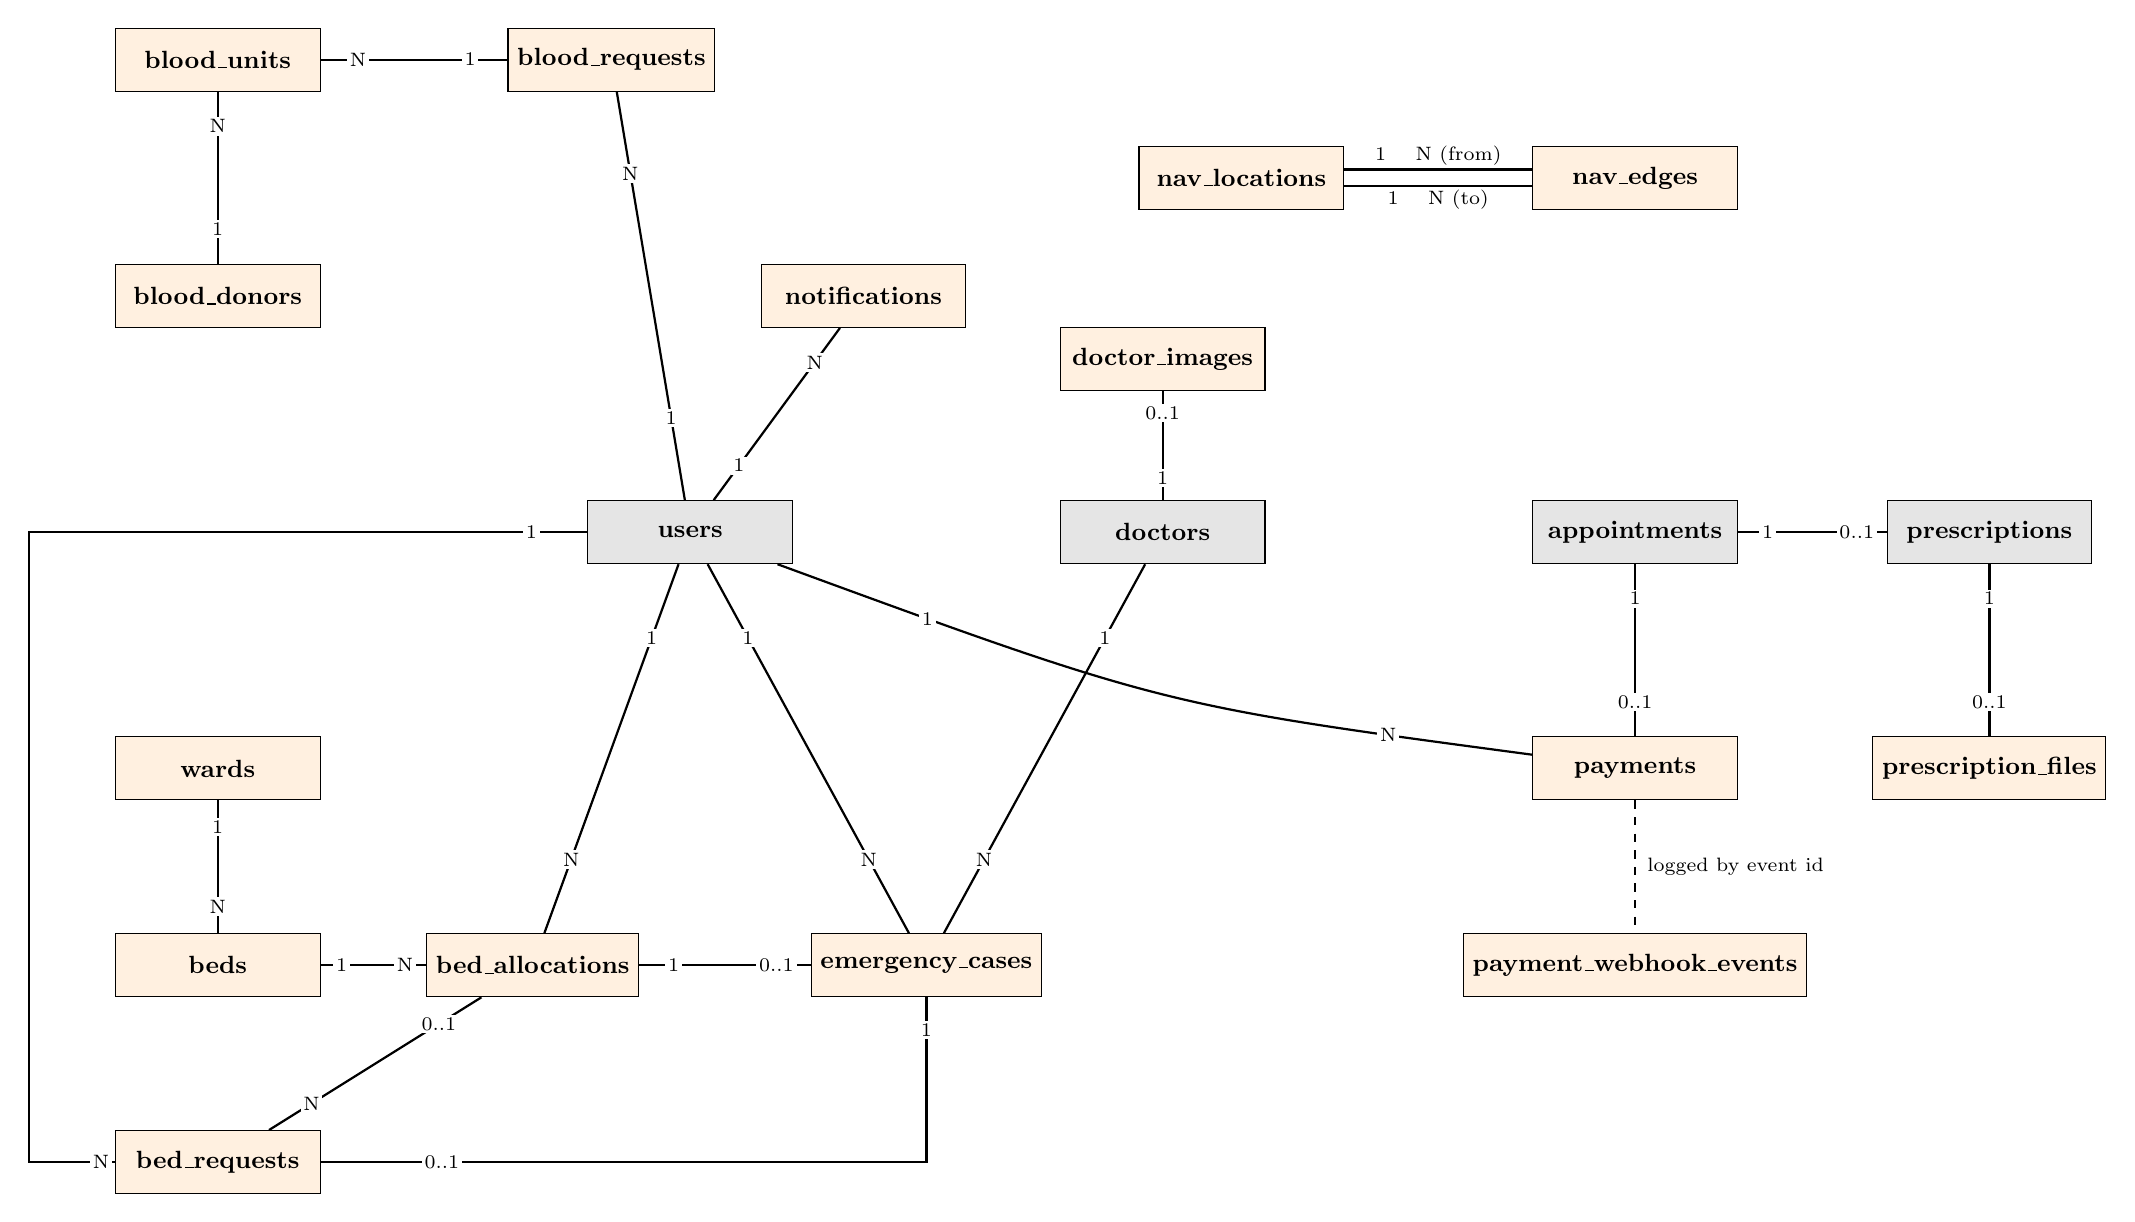
\begin{tikzpicture}[
  ent/.style={rectangle, draw=black, minimum width=2.6cm, minimum height=0.8cm, align=center, font=\small\bfseries, fill=orange!12},
  core/.style={ent, fill=gray!20},
  lin/.style={-, thick},
  card/.style={font=\scriptsize, fill=white, inner sep=1pt}
]
\node[core] (users) at (0,0) {users};
\node[core] (doctors) at (6,0) {doctors};
\node[core] (appts) at (12,0) {appointments};

\node[ent] (wards) at (-6,-3) {wards};
\node[ent] (beds) at (-6,-5.5) {beds};
\node[ent] (alloc) at (-2,-5.5) {bed\_allocations};
\node[ent] (er) at (3,-5.5) {emergency\_cases};
\node[ent] (notif) at (2.2,3) {notifications};
\node[ent] (donors) at (-6,3) {blood\_donors};
\node[ent] (units) at (-6,6) {blood\_units};
\node[ent] (breq) at (-1,6) {blood\_requests};
\node[ent] (pay) at (12,-3) {payments};
\node[ent] (wh) at (12,-5.5) {payment\_webhook\_events};
\node[ent] (loc) at (7,4.5) {nav\_locations};
\node[ent] (bedreq) at (-6,-8) {bed\_requests};
\node[core] (pres) at (16.5,0) {prescriptions};
\node[ent] (pfile) at (16.5,-3) {prescription\_files};
\node[ent] (dimg) at (6,2.2) {doctor\_images};
\node[ent] (edge) at (12,4.5) {nav\_edges};

\draw[lin] (wards) -- node[card,pos=0.2]{1} node[card,pos=0.8]{N} (beds);
\draw[lin] (beds) -- node[card,pos=0.2]{1} node[card,pos=0.8]{N} (alloc);
\draw[lin] (users) -- node[card,pos=0.2]{1} node[card,pos=0.8]{N} (alloc);
\draw[lin] (alloc) -- node[card,pos=0.2]{1} node[card,pos=0.8]{0..1} (er);
\draw[lin] (users) -- node[card,pos=0.2]{1} node[card,pos=0.8]{N} (er);
\draw[lin] (doctors) -- node[card,pos=0.2]{1} node[card,pos=0.8]{N} (er);
\draw[lin] (users) -- node[card,pos=0.2]{1} node[card,pos=0.8]{N} (notif);
\draw[lin] (donors) -- node[card,pos=0.2]{1} node[card,pos=0.8]{N} (units);
\draw[lin] (breq) -- node[card,pos=0.2]{1} node[card,pos=0.8]{N} (units);
\draw[lin] (users) -- node[card,pos=0.2]{1} node[card,pos=0.8]{N} (breq);
\draw[lin] (appts) -- node[card,pos=0.2]{1} node[card,pos=0.8]{0..1} (pay);
\draw[lin] (users) .. controls (6,-2.2) .. node[card,pos=0.15]{1} node[card,pos=0.85]{N} (pay);
\draw[lin, dashed] (pay) -- node[card, right=3pt]{logged by event id} (wh);
\draw[lin] (bedreq) -- node[card,pos=0.2]{N} node[card,pos=0.8]{0..1} (alloc);
\draw[lin] (bedreq.east) -| node[card,pos=0.1]{0..1} node[card,pos=0.9]{1} (er.south);
\draw[lin] (users.west) -- node[card,pos=0.1]{1} (-8.4,0) |- node[card,pos=0.92]{N} (bedreq.west);
\draw[lin] (appts) -- node[card,pos=0.2]{1} node[card,pos=0.8]{0..1} (pres);
\draw[lin] (pres) -- node[card,pos=0.2]{1} node[card,pos=0.8]{0..1} (pfile);
\draw[lin] (doctors) -- node[card,pos=0.2]{1} node[card,pos=0.8]{0..1} (dimg);
\draw[lin] ([yshift=3pt]loc.east) -- node[card,above]{1 \quad N (from)} ([yshift=3pt]edge.west);
\draw[lin] ([yshift=-3pt]loc.east) -- node[card,below]{1 \quad N (to)} ([yshift=-3pt]edge.west);
\end{tikzpicture}%
}
\caption{Extended Entity-Relationship Diagram for the Enhanced Modules}
\label{fig:er-ext}
\end{figure}

\FloatBarrier
\section{Module Design}

\subsection{Authentication Module}

Authentication includes user registration (only for patients) and login for all users. In the first version, a single JSON Web Token was returned to the client, stored in \texttt{localStorage}, and sent in the \texttt{Authorization: Bearer} header. Because any script running on the page can read \texttt{localStorage}, a single cross-site scripting flaw would have exposed every session. In version 2, after a successful login the server issues two tokens and sets them as \emph{httpOnly} cookies that JavaScript cannot read: a short-lived \textbf{access token} (15 minutes, carrying \texttt{id}, \texttt{email}, \texttt{role} and \texttt{type: 'access'}) sent with every request, and a \textbf{refresh token} (7 days, \texttt{type: 'refresh'}) whose cookie path is restricted to \texttt{/api/auth}. When the access token expires, the frontend calls \texttt{POST /api/auth/refresh} once, receives a new pair of tokens (the refresh token is rotated), and retries the original request. \texttt{GET /api/auth/me} restores the session on page reload, and \texttt{POST /api/auth/logout} clears both cookies.

On the server side, the authentication middleware reads the access-token cookie, verifies its signature and expiry with \texttt{jsonwebtoken.verify()}, rejects tokens whose \texttt{type} is not \texttt{access}, and attaches the decoded payload to \texttt{req.user}. Then the \texttt{requireRole(...roles)} middleware checks whether the user's role is one of the roles allowed for the route (several modules, such as emergency, are shared by doctors and administrators). Otherwise, it returns a \texttt{403 Forbidden} response. Because cookies are sent automatically by the browser, every state-changing request must also carry a CSRF token, as described in Section~\ref{sec:security}.

\subsection{Appointment Booking Module}

Here is how the patient books an appointment: (1) patient chooses a specialization and sends a \texttt{GET /api/doctors?specialization=X} request; (2) when choosing a doctor, the patient selects a date, which triggers the request \texttt{GET /api/slots?doctorId=Y\&date=Z}; (3) finally, the patient books a chosen slot by sending \texttt{POST /api/appointments/book} with the JSON body \texttt{\{doctorId, slotId, reason, consultationType\}}, where \texttt{consultationType} is \texttt{in\_person} or \texttt{video}. The slot booking controller wraps these operations in a database transaction in order to avoid any race conditions. Inside the transaction the server also enforces the booking rules: the slot must be free, not blocked and not in the past; the date must lie between today and 13 days ahead; a patient may hold at most five upcoming appointments and at most one with the same doctor on the same day. For a video visit it also generates a random, unguessable room name. After the transaction commits, a confirmation notification is sent to both the patient and the doctor, and the cached availability for that doctor and date is invalidated.

An appointment has a deliberately small life cycle (Figure~\ref{fig:apptstates}): it is \texttt{pending} until it is completed or cancelled, and it can never be reopened. A visit can be completed only from 15 minutes before its start, which is when the video room opens; cancelling frees the slot for another patient and, for a paid visit, marks the payment for refund.

\begin{figure}[H]
\centering
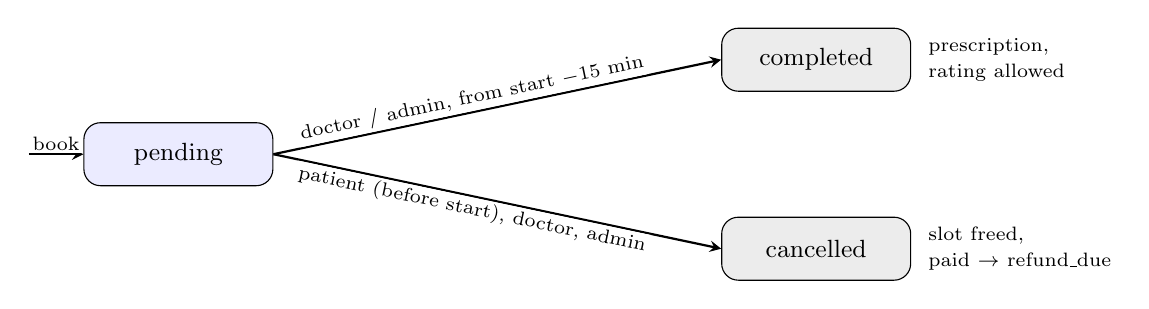
\begin{tikzpicture}[
  st/.style={draw, rounded corners=6pt, minimum width=2.4cm, minimum height=0.8cm, align=center, font=\small, fill=blue!8},
  fin/.style={st, fill=gray!15},
  arr/.style={->, >=stealth, thick},
  lbl/.style={font=\scriptsize, fill=white, inner sep=1pt, align=center}
]
\node[st] (p) at (0,0) {pending};
\node[fin] (c) at (8.1,1.2) {completed};
\node[fin] (x) at (8.1,-1.2) {cancelled};
\draw[arr] (-1.9,0) -- node[lbl, above]{book} (p);
\draw[arr] (p.east) -- node[lbl, sloped, above, pos=0.45]{doctor / admin, from start $-$15 min} (c.west);
\draw[arr] (p.east) -- node[lbl, sloped, below, pos=0.45]{patient (before start), doctor, admin} (x.west);
\node[font=\scriptsize, align=left, anchor=west] at (9.4,-1.2) {slot freed,\\paid $\rightarrow$ refund\_due};
\node[font=\scriptsize, align=left, anchor=west] at (9.4,1.2) {prescription,\\rating allowed};
\end{tikzpicture}
\caption{Appointment Life Cycle}
\label{fig:apptstates}
\end{figure}

\subsection{Slot Generation Module}

The \texttt{generateSlots} function creates 15-minute slots for all the registered doctors from 09:00 to 16:45 (32 slots per day) on a specified date, using \texttt{INSERT IGNORE} with a single multi-row statement so that it is idempotent. The application runs this function when starting up for the next 14 days and schedules it for daily midnight execution via \texttt{node-cron} package. A separate database cleanup query removes past slots that no appointment refers to, in order to prevent \texttt{doctor\_slots} table bloating; a slot that a cancelled appointment still points to is kept, so the visit history stays intact. A failed cleanup is logged and never stops the generation of the next 14 days. Slots are created only inside the booking window, so a request for a date outside it cannot create rows, and blocking a day marks its slots unavailable instead of deleting them, so the midnight generator cannot reopen a blocked day.

\subsection{MediBot AI Chatbot Module}

MediBot is built upon the Gemini 2.5 Flash language model \cite{geminidocs} (Gemini 1.5 Flash in the first version). By means of a specifically crafted system prompt, we constrained the model to perform a limited set of 5 actions: (1) answer general health questions, (2) recommend medical specializations according to symptom descriptions, (3) provide guidance on booking an appointment, (4) provide the information about the hospital and its services, (5) get the patient's appointment history. In the end of the answer, the model provides structured action block \texttt{>>>ACTION:\{"type":XXX\}} that allows triggering corresponding interactions in the UI part. When the patient confirms a booking in the chat, the widget calls the same \texttt{POST /api/appointments/book} endpoint as the booking page and lists only slots that can really be booked, so MediBot is subject to exactly the same rules. The public chat endpoint is rate-limited to 20 messages per minute per client because every message calls a paid external API.

\subsection{Notification Module}

The notification module is a small shared service used by every other module. \texttt{notifyUsers(ids, \{type, title, message, link\})} inserts one row per recipient in a single multi-row statement; \texttt{notifyRoles(roles, ...)} fans a message out to every user of the given roles (for example, an ESI level 1 or 2 arrival alerts every doctor and administrator). Both helpers are deliberately \emph{fire-and-forget safe}: they catch and log their own errors, so that a failure to write a notification can never undo or block the clinical action that triggered it. They are always called \emph{after} the surrounding database transaction has committed, so a notification is never sent for an action that was later rolled back.

\subsection{Enhanced Module Overview}

The seven modules added in this phase follow the same layered pattern as the core: a route file declares the role guards and validation schemas, a controller handles the HTTP request, and a service or utility module holds the business rules so that they can be unit-tested without a database. Their detailed design and implementation are presented in Chapter~\ref{ch:modules}; Table~\ref{tab:modules} gives a summary.

\begin{table}[H]
\centering
\caption{Enhanced Modules: Users, Tables and Core Rules}
\label{tab:modules}
\renewcommand{\arraystretch}{1.25}
\begin{tabular}{|L{2.4cm}|L{2.3cm}|L{3.7cm}|L{5.0cm}|}
\hline
\rowcolor{blue!12}
\textbf{Module} & \textbf{Users} & \textbf{Tables} & \textbf{Core rule} \\
\hline
Blood Bank & Admin (all), Doctor (stock, requests) & blood\_donors, blood\_units, blood\_requests & Compatible units only, exact group first, earliest expiry first; 56-day donor interval \\
\hline
Bed Management & Admin (assign), Doctor (request) & wards, beds, bed\_allocations, bed\_requests & Doctors request, admin assigns; one open allocation per bed and per patient and one pending request of each kind, enforced by unique keys \\
\hline
Emergency & Admin, Doctor & emergency\_cases & ESI level 1--5, queue by level then arrival, fixed status transitions \\
\hline
Teleconsultation & Patient, Doctor & appointments (video columns) & Only the booked pair may join; patient must have paid and waits until the doctor admits; window $-15$ to $+60$ minutes; signed room tokens \\
\hline
Notifications & All signed-in users & notifications & Written after commit; failures never break the triggering action \\
\hline
Navigation & Public (read), Admin (edit) & nav\_locations, nav\_edges & Dijkstra shortest path; accessible mode removes stair edges \\
\hline
Payments & Patient, Admin & payments, payment\_webhook\_events & Amount from DB, HMAC signature check, webhook processed once \\
\hline
\end{tabular}
\end{table}

\FloatBarrier
\section{API Design}

Table~\ref{tab:api} presents the complete REST API endpoint reference for the Care \& Cure HMS. All endpoints return a uniform JSON envelope, \texttt{\{success, data\}} on success and \texttt{\{success: false, message, error: \{code, message\}\}} on failure, so that the frontend handles errors in one place. Path parameters, query strings and bodies are validated by Zod schemas before the controller runs; an invalid request receives \texttt{400} with the list of failing fields.

\begin{longtable}{|L{1.9cm}|L{5.4cm}|L{2.1cm}|L{3.8cm}|}
\caption{REST API Endpoint Reference} \label{tab:api} \\
\hline
\textbf{Method} & \textbf{Endpoint} & \textbf{Auth/Role} & \textbf{Description} \\
\hline
\endfirsthead
\hline
\textbf{Method} & \textbf{Endpoint} & \textbf{Auth/Role} & \textbf{Description} \\
\hline
\endhead
POST & /api/auth/register & Public & Patient self-registration \\
\hline
POST & /api/auth/login & Public & All roles login, returns JWT \\
\hline
GET & /api/patient/profile & Patient & Fetch own profile \\
\hline
PUT & /api/patient/profile & Patient & Update own profile \\
\hline
GET & /api/patient/appointments & Patient & Fetch appointment history \\
\hline
GET & /api/patient/medical-history & Patient & Fetch prescription history \\
\hline
POST & /api/patient/rate & Patient & Submit doctor rating \\
\hline
GET & /api/doctors & Public & List doctors by specialization \\
\hline
GET & /api/slots & Public & Get available slots by doctor/date \\
\hline
POST & /api/appointments/book & Patient & Book a slot \\
\hline
GET & /api/doctor/appointments & Doctor & Doctor's appointment list \\
\hline
GET & /api/doctor/dashboard & Doctor & Dashboard stats \\
\hline
PUT & /api/doctor/appointment-status & Doctor & Update appointment status \\
\hline
POST & /api/doctor/prescription & Doctor & Upload prescription \\
\hline
POST & /api/doctor/slots & Doctor & Create additional slots \\
\hline
GET & /api/admin/users & Admin & List users (v2: server-side search, sort, paging) \\
\hline
POST & /api/admin/doctors & Admin & Create doctor account \\
\hline
PATCH & /api/admin/doctors/:id & Admin & Update doctor details \\
\hline
DELETE & /api/admin/user/:id & Admin & Delete a user \\
\hline
GET & /api/admin/appointments & Admin & List appointments (v2: search, filter, paging) \\
\hline
PATCH & /api/admin/appointments/:id & Admin & Complete or cancel (frees the slot) \\
\hline
DELETE & /api/admin/appointments/:id & Admin & Delete appointment \\
\hline
GET & /api/admin/slots & Admin & View slots by doctor/date \\
\hline
PATCH & /api/admin/slots/:id/toggle & Admin & Toggle slot availability \\
\hline
POST & /api/admin/slots/generate & Admin & Manually trigger slot generation \\
\hline
DELETE & /api/admin/slots/day & Admin & Block a day (slots marked unavailable, not deleted) \\
\hline
POST & /api/chatbot/message & Public & Send message to MediBot \\
\hline
GET & /api/chatbot/doctors & -- & Removed in v2; MediBot uses /api/doctors \\
\hline
GET & /api/chatbot/slots & -- & Removed in v2; MediBot uses /api/slots \\
\hline
POST & /api/chatbot/book & -- & Removed in v2; MediBot books through /api/appointments/book \\
\hline
GET & /api/chatbot/appointments & Patient & View appointments via chatbot \\
\hline
\rowcolor{orange!12} \multicolumn{4}{|l|}{\textbf{Endpoints added in version 2}} \\
\hline
POST & /api/auth/refresh & Cookie & Rotate refresh token, new access token \\
\hline
POST & /api/auth/logout & Cookie & Clear session cookies \\
\hline
GET & /api/auth/me & Any role & Current user (session restore) \\
\hline
GET & /api/admin/doctors & Admin & List doctors \\
\hline
PATCH & /api/admin/users/:id & Admin & Update a user \\
\hline
GET & /api/notifications & Any role & List own notifications, unread count \\
\hline
PATCH & /api/notifications/:id/read & Any role & Mark one as read \\
\hline
PATCH & /api/notifications/read-all & Any role & Mark all as read \\
\hline
GET & /api/beds/wards & Admin, Doctor & Wards with occupancy counts \\
\hline
POST & /api/beds/wards & Admin & Create ward \\
\hline
GET & /api/beds/stats & Admin, Doctor & Hospital occupancy statistics \\
\hline
GET & /api/beds & Admin & Bed grid with patients and pending discharge requests \\
\hline
POST & /api/beds & Admin & Create bed \\
\hline
PATCH & /api/beds/:id/status & Admin & Set maintenance/reserved/available \\
\hline
GET & /api/beds/patients/search & Admin, Doctor & Find a patient by name/email/phone \\
\hline
POST & /api/beds/:id/allocate & Admin & Admit patient to bed (answers a pending request) \\
\hline
POST & /api/beds/allocations/:id/discharge & Admin & Discharge and free the bed \\
\hline
GET & /api/beds/my-patients & Doctor & Beds of the doctor's admitted patients \\
\hline
GET, POST & /api/beds/requests & Admin, Doctor & List / raise bed or discharge requests \\
\hline
POST & /api/beds/requests/:id/fulfill & Admin & Assign a bed or discharge \\
\hline
PATCH & /api/beds/requests/:id/reject & Admin & Reject with a reason \\
\hline
PATCH & /api/beds/requests/:id/cancel & Admin, Doctor & Cancel a pending request \\
\hline
GET & /api/blood/inventory & Admin, Doctor & Stock by group and component \\
\hline
GET, POST & /api/blood/donors & Admin & List / register donors \\
\hline
POST & /api/blood/donations & Admin & Record a donation (creates a unit) \\
\hline
GET & /api/blood/units & Admin & List units \\
\hline
PATCH & /api/blood/units/:id/discard & Admin & Discard a unit \\
\hline
GET, POST & /api/blood/requests & Admin, Doctor & List / raise blood requests \\
\hline
POST & /api/blood/requests/:id/fulfill & Admin & Issue compatible units (FEFO) \\
\hline
PATCH & /api/blood/requests/:id/reject & Admin & Reject with a note \\
\hline
PATCH & /api/blood/requests/:id/cancel & Admin, Doctor & Cancel a pending request \\
\hline
GET & /api/emergency/stats & Admin, Doctor & Open cases per ESI level \\
\hline
GET, POST & /api/emergency/cases & Admin, Doctor & Queue / register an arrival \\
\hline
GET, PATCH & /api/emergency/cases/:id & Admin, Doctor & View / update status, level, doctor \\
\hline
POST & /api/emergency/cases/:id/admit & Admin & Admit directly to a bed \\
\hline
POST & /api/emergency/cases/:id/request-bed & Doctor & Emergency bed request for the case \\
\hline
GET & /api/teleconsult/:appointmentId/join & Patient, Doctor & Waiting state, or room and token \\
\hline
GET & /api/teleconsult/:appointmentId/status & Doctor & Is the patient waiting / admitted \\
\hline
POST & /api/teleconsult/:appointmentId/admit & Doctor & Let the waiting patient in \\
\hline
PATCH & /api/teleconsult/:appointmentId/complete & Doctor & Mark video visit completed \\
\hline
GET & /api/navigation/locations & Public & List locations \\
\hline
GET & /api/navigation/route & Public & Shortest / accessible route \\
\hline
POST, DELETE & /api/navigation/locations[/:id] & Admin & Edit locations \\
\hline
POST, DELETE & /api/navigation/edges[/:id] & Admin & Edit connections \\
\hline
POST & /api/payments/orders & Patient & Create or reuse a payment order \\
\hline
POST & /api/payments/verify & Patient & Verify checkout signature \\
\hline
POST & /api/payments/orders/:orderId/fail & Patient & Record a failed attempt \\
\hline
GET & /api/payments/my & Patient & Own payment history \\
\hline
GET & /api/payments & Admin & Paginated ledger with totals \\
\hline
POST & /api/payments/webhook & HMAC & Razorpay webhook (signature-verified) \\
\hline
POST & /api/patient/appointments/:id/cancel & Patient & Cancel before the start time \\
\hline
GET & /api/files/prescriptions/:id & Patient, Doctor & Prescription file (own only, else 404) \\
\hline
GET & /api/files/doctors/:id/image & Public & Doctor photo \\
\hline
GET & /api/health & Public & Liveness and database check \\
\hline
\end{longtable}

\FloatBarrier
\section{Role-Based Access Matrix}

Table~\ref{tab:rbac} summarises which role can perform which action across the platform. It is enforced on the server by the \texttt{requireRole} middleware on each route, and mirrored on the client, where each portal's routes send a user of another role back to their own section and admin-only buttons are hidden; the client-side checks are a convenience, never a security boundary.

\begin{table}[H]
\centering
\caption{Role-Based Access Matrix}
\label{tab:rbac}
\renewcommand{\arraystretch}{1.2}
\begin{tabular}{|L{6.2cm}|C{1.5cm}|C{1.5cm}|C{1.5cm}|C{1.5cm}|}
\hline
\rowcolor{blue!12}
\textbf{Action} & \textbf{Visitor} & \textbf{Patient} & \textbf{Doctor} & \textbf{Admin} \\
\hline
Browse doctors and free slots, chat with MediBot & \checkmark & \checkmark & \checkmark & \checkmark \\
\hline
Indoor navigation (find a route) & \checkmark & \checkmark & \checkmark & \checkmark \\
\hline
Book appointment, rate doctor, view own history & $\times$ & \checkmark & $\times$ & $\times$ \\
\hline
Cancel an appointment & $\times$ & Own, before start & Own & \checkmark \\
\hline
Open a prescription file & $\times$ & Own & Own & $\times$ \\
\hline
Pay consultation fee, view own payments & $\times$ & \checkmark & $\times$ & $\times$ \\
\hline
Join video consultation & $\times$ & Own, paid, after admit & Own, admits & $\times$ \\
\hline
Complete visit, upload prescription (from 15 min before start) & $\times$ & $\times$ & Own & Complete only \\
\hline
Request a bed or a discharge, view own patients' beds & $\times$ & $\times$ & \checkmark & $\times$ \\
\hline
View full bed grid, assign beds, discharge, answer requests & $\times$ & $\times$ & $\times$ & \checkmark \\
\hline
Create wards and beds, change bed status & $\times$ & $\times$ & $\times$ & \checkmark \\
\hline
View blood stock, raise and cancel requests & $\times$ & $\times$ & \checkmark & \checkmark \\
\hline
Manage donors, record donations, issue or reject & $\times$ & $\times$ & $\times$ & \checkmark \\
\hline
Emergency board: register, triage, treat, close & $\times$ & $\times$ & \checkmark & \checkmark \\
\hline
Emergency admission & $\times$ & $\times$ & Request bed & Admit \\
\hline
Edit navigation map, view payment ledger, manage users and slots & $\times$ & $\times$ & $\times$ & \checkmark \\
\hline
Receive in-app notifications & $\times$ & \checkmark & \checkmark & \checkmark \\
\hline
\end{tabular}
\end{table}

\FloatBarrier
\section{Concurrency and Data Integrity Design}

Several workflows in a hospital are naturally concurrent: two receptionists may try to admit patients to the last ICU bed, two patients may click the same slot, or a payment webhook may arrive while the patient's browser is verifying the same payment. The design follows three rules, drawn from classical transaction processing \cite{gray1992}:

\begin{enumerate}
    \item \textbf{Lock the row you are about to change.} Every read-modify-write runs in a transaction that reads the target row with \texttt{SELECT ... FOR UPDATE}. Other transactions that want the same row wait until the first commits, and then see the new state.
    \item \textbf{Always lock in the same order.} Deadlocks happen when two transactions lock the same rows in opposite orders. The documented lock orders are \emph{bed request $\rightarrow$ emergency case $\rightarrow$ bed $\rightarrow$ patient user $\rightarrow$ allocation} for admissions, \emph{appointment $\rightarrow$ payment} for payments, and \emph{appointment $\rightarrow$ slot} for cancellation (booking never holds an appointment lock while it takes a slot). Queries that would also lock a joined row (\texttt{JOIN ... FOR UPDATE}) are split into a locked read and a separate unlocked read. If MySQL still reports a deadlock, the shared \texttt{inTransaction} helper retries the whole transaction up to two times on a fresh connection.
    \item \textbf{Let the database have the last word.} Application checks give friendly error messages, but unique keys guarantee correctness: \texttt{appointments.active\_slot\_id} is unique while a visit is live, \texttt{bed\_requests.open\_key} allows one pending request of each kind, \texttt{payments.appointment\_id} and \texttt{provider\_order\_id} are unique, \texttt{payment\_webhook\_events.event\_id} is unique, and \texttt{bed\_allocations} has unique \texttt{open\_bed\_id} and \texttt{open\_patient\_id} columns. A violated key is translated into a \texttt{409 Conflict} response instead of a server error.
\end{enumerate}

Side effects outside the database, such as notifications and calls to the payment gateway, are never performed inside a transaction, because a retried transaction would repeat them and a long external call would hold locks for its whole duration.


\chapter{Implementation and Results}
\label{ch:impl}
\lhead{\emph{Chapter 4: Implementation and Results}}
\FloatBarrier
\section{Development Environment}

The system was developed using the following environment configuration:

\begin{itemize}
    \item \textbf{Operating System}: macOS / Windows 11
    \item \textbf{Code Editor}: Visual Studio Code
    \item \textbf{Database}: MySQL 8.0 / MariaDB via XAMPP / MAMP locally; MySQL 8 on Aiven in production
    \item \textbf{Cache}: Redis 7 (optional locally; started by \texttt{docker-compose})
    \item \textbf{Node.js Version}: v20 LTS
    \item \textbf{Package Manager}: npm
    \item \textbf{API Testing}: Postman, Jest + Supertest
    \item \textbf{Browser Testing}: Playwright with system Chrome
    \item \textbf{Version Control}: Git / GitHub, feature branches merged through pull requests with CI checks
\end{itemize}

The frontend development server runs on \texttt{http://localhost:5173} (Vite) and the backend Express server on \texttt{http://localhost:5001}. CORS is configured to allow credentialed cross-origin requests only from the configured frontend origin. The backend process and its database session both run in the Asia/Kolkata time zone (Section~\ref{sec:tz}).

\FloatBarrier
\section{Backend Implementation}

\FloatBarrier
\subsection{Project Structure}

The backend is organized following the MVC (Model-View-Controller) pattern adapted for RESTful APIs:

\begin{lstlisting}[language=bash, caption=Backend Directory Structure]
backend/
  server.js          # Entry point: listen, cron jobs, graceful exit
  app.js             # Express app and middleware chain (used by tests)
  config/
    db.js            # MySQL pool, session time zone
    redis.js         # ioredis client (fails open)
  routes/            # 14 route files: auth, patient, doctor,
                     # appointment, admin, chatbot, notification,
                     # bed, bloodBank, emergency, teleconsult,
                     # navigation, payment, file
  controllers/       # one controller per route file
  services/
    appointmentService.js bedService.js
    bedRequestService.js  bloodBankService.js
    notificationService.js paymentGateway.js
  validators/        # Zod schemas per module
  middleware/
    auth.js  role.js  csrf.js  rateLimiter.js
    validate.js  upload.js  errorHandler.js
  utils/
    generateSlots.js  transaction.js  errors.js
    triage.js  bloodCompatibility.js  pathfinding.js
    cache.js  cookies.js  dates.js  sql.js
    videoAccess.js
  database/
    schema.sql  migration_*.sql  applySchema.js
    seedDemo.js        # optional demo data
  tests/
    unit/  integration/  helpers/  setup/
  Dockerfile  start.sh
\end{lstlisting}

\FloatBarrier
\subsection{Database Connection Pool}

The MySQL connection pool is configured with a limit of 10 concurrent connections, ensuring efficient handling of parallel API requests without exhausting database resources. Managed databases require TLS, which is enabled with \texttt{DB\_SSL=true} and, when available, verified against the provider's CA certificate. Every new connection first pins its session time zone to IST, so that \texttt{NOW()} on a UTC cloud server agrees with the slot times stored in IST; if this fails, the connection is destroyed rather than used with the wrong zone.

\begin{lstlisting}[language=JavaScript, caption=MySQL Connection Pool Configuration]
const pool = mysql.createPool({
  host: process.env.DB_HOST,
  port: process.env.DB_PORT ? parseInt(process.env.DB_PORT, 10) : undefined,
  user: process.env.DB_USER,
  password: process.env.DB_PASSWORD,
  database: process.env.DB_NAME,
  waitForConnections: true,
  connectionLimit: 10,
  queueLimit: 0,
  ...(useSSL && { ssl: sslOption }),
});
pool.on('connection', (conn) => conn.query(`SET time_zone = '+05:30'`, (err) => {
  if (err) conn.destroy();   // never serve queries in the wrong zone
}));
const db = pool.promise();
\end{lstlisting}

\FloatBarrier
\subsection{Authentication Implementation}

Password hashing uses bcryptjs, providing a good balance between security strength and computation time. In version 1 a single JWT with a 7-day expiry was returned to the client. Version 2 issues a 15-minute access token and a 7-day refresh token and stores both in httpOnly cookies, so they are invisible to JavaScript:

\begin{lstlisting}[language=JavaScript, caption=Session Cookies (utils/cookies.js)]
const baseOptions = {
  httpOnly: true,
  secure: isProd,                     // HTTPS only in production
  sameSite: isProd ? 'none' : 'lax',  // frontend and API on different domains
};
res.cookie('access_token', accessToken,
  { ...baseOptions, path: '/', maxAge: 15 * 60 * 1000 });
res.cookie('refresh_token', refreshToken,     // only sent to /api/auth/*
  { ...baseOptions, path: '/api/auth', maxAge: 7 * 24 * 60 * 60 * 1000 });
\end{lstlisting}

The authentication middleware verifies the access-token cookie on every protected request and attaches the decoded payload to \texttt{req.user}. The role middleware immediately follows. It now accepts a list of roles, because several modules are shared by doctors and administrators:

\begin{lstlisting}[language=JavaScript, caption=Role Enforcement Middleware]
const requireRole = (...roles) => (req, res, next) => {
  if (!req.user || !roles.includes(req.user.role))
    return next(new ForbiddenError('You do not have access to this resource.'));
  next();
};
// e.g. router.use(auth, requireRole('admin', 'doctor'));
\end{lstlisting}

\FloatBarrier
\subsection{Appointment Booking Transaction}

To prevent race conditions in concurrent bookings of the same slot, the booking controller uses a database transaction with a check-before-insert pattern. In version 2 this pattern is provided by the shared \texttt{inTransaction} helper (Section~\ref{sec:txhelper}); the essential steps are:

\begin{lstlisting}[language=JavaScript, caption=Atomic Appointment Booking with Transaction]
const conn = await db.getConnection();
await conn.beginTransaction();
const [slot] = await conn.query(
  'SELECT * FROM doctor_slots WHERE id=? AND is_booked=0 FOR UPDATE',
  [slotId]);
if (!slot.length) throw new Error('Slot already booked');
await conn.query('UPDATE doctor_slots SET is_booked=1 WHERE id=?',[slotId]);
await conn.query('INSERT INTO appointments ... VALUES (...)',[...]);
await conn.commit();
\end{lstlisting}

The \texttt{FOR UPDATE} lock ensures that between the check and the insert, no other transaction can book the same slot.

\FloatBarrier
\subsection{Automated Slot Generation}

The slot generation utility creates 15-minute intervals from 09:00 to 16:45 (32 slots) for every registered doctor on a given date. An \texttt{INSERT IGNORE} statement against the \texttt{UNIQUE(doctor\_id, date, time)} key ensures no duplicates are created. In version 2 the 32 rows for a doctor are inserted with one multi-row statement instead of 32 separate queries.
\begin{lstlisting}[language=JavaScript, caption=Slot Generation Logic (Simplified)]
function buildTimeSlots() {
  const slots = [];
  for (let hour = 9; hour < 17; hour++)
    for (let min = 0; min < 60; min += 15)
      slots.push(`${pad(hour)}:${pad(min)}:00`);
  return slots; // 32 slots
}
async function generateSlotsForDoctorDate(doctorId, date) {
  const values = buildTimeSlots().map(t => [doctorId, date, t, 0, 1]);
  await db.query(`INSERT IGNORE INTO doctor_slots
    (doctor_id, date, time, is_booked, is_available) VALUES ?`, [values]);
}
\end{lstlisting}

The \texttt{node-cron} schedule triggers this utility at midnight daily and also cleans up past unbooked slots:

\begin{lstlisting}[language=JavaScript, caption=Cron Job for Daily Slot Management]
async function maintainSlots(when) {       // at start-up and at midnight
  try { await cleanupPastSlots(); }         // a failure must not skip
  catch (err) { console.error(when, err); } // the next 14 days
  try { await generateRollingSlots(14); }
  catch (err) { console.error(when, err); }
}
cron.schedule('0 0 * * *', () => maintainSlots('Cron'));

// cleanupPastSlots: keep any slot an appointment still points to
DELETE s FROM doctor_slots s
 WHERE s.date < CURDATE() AND s.is_booked = 0
   AND NOT EXISTS (SELECT 1 FROM appointments a WHERE a.slot_id = s.id)
\end{lstlisting}

\FloatBarrier
\subsection{Prescription File Upload}

In the first version, Multer saved prescription files to an \texttt{uploads/} folder that was served as public static files, and the type was checked only from the file name. A review found two problems with this design: anyone who learnt a file's URL could download another patient's prescription, and the free hosting plan wipes the container's disk on every restart, so files disappeared. Version 2 changes the design in three ways:

\begin{itemize}
    \item \textbf{Stored in the database.} Multer keeps the upload in memory, and the controller writes it into the \texttt{prescription\_files} or \texttt{doctor\_images} table in the same transaction as the prescription. Prescription files are limited to 5~MB and photos to 2~MB.
    \item \textbf{Type checked by content.} The real type is detected from the file's first bytes (its ``magic number''), never from the name or the type claimed by the browser, so a script renamed to \texttt{.pdf} is rejected. The stored name is sanitised.
    \item \textbf{Served only to its owners.} \texttt{GET /api/files/prescriptions/:id} joins the file to its prescription and returns it only to that prescription's patient or doctor, with \texttt{Cache-Control: private, no-store} and \texttt{X-Content-Type-Options: nosniff}. Anyone else receives \texttt{404}, so the file's existence is not revealed. The public \texttt{/uploads} folder no longer exists.
\end{itemize}

\begin{lstlisting}[language=JavaScript, caption=Upload Type Detection by File Signature (middleware/upload.js; simplified)]
const SIGNATURES = [
  { mime: 'application/pdf', test: (b) => b.subarray(0, 5).toString('latin1') === '%PDF-' },
  { mime: 'image/png',  test: (b) => b.subarray(0, 8).equals(PNG_MAGIC) },
  { mime: 'image/jpeg', test: (b) => b[0] === 0xff && b[1] === 0xd8 && b[2] === 0xff },
  { mime: 'image/webp', test: (b) => b.subarray(0, 4).toString('latin1') === 'RIFF'
                                  && b.subarray(8, 12).toString('latin1') === 'WEBP' },
];
const detectMime = (buf) =>
  SIGNATURES.find((s) => buf.length >= 12 && s.test(buf))?.mime ?? null;
\end{lstlisting}

A prescription's patient is always taken from its appointment, never from the request body, re-saving a prescription without a new file keeps the existing file, and a cancelled visit cannot be prescribed or completed. Patients' pages keep the line breaks of the doctor's notes, so structured prescriptions (diagnosis, medicines, advice, follow-up) remain readable.

\FloatBarrier
\subsection{Request Validation with Zod}

Every route that accepts input declares a Zod schema for its body, query string or path parameters, and the generic \texttt{validate(schema, source)} middleware rejects invalid requests with \texttt{400} before any controller code runs. Schemas also coerce and normalise values (for example query strings to numbers) and supply defaults, so controllers work only with clean, typed data. The same schemas document the API contract in code.

\begin{lstlisting}[language=JavaScript, caption=Validation Schema and Route (payments)]
const listPaymentsQuerySchema = z.object({
  page:  z.coerce.number().int().min(1).max(10000).default(1),
  limit: z.coerce.number().int().min(1).max(100).default(50),
});
router.get('/', requireRole('admin'),
  validate(v.listPaymentsQuerySchema, 'query'), c.listPayments);
\end{lstlisting}

\FloatBarrier
\subsection{Centralised Error Handling}

Controllers do not build error responses themselves. They throw typed errors (\texttt{ValidationError} 400, \texttt{AuthError} 401, \texttt{ForbiddenError} 403, \texttt{NotFoundError} 404, \texttt{ConflictError} 409, or a generic \texttt{AppError} with any status and machine-readable code, such as \texttt{402 PAYMENT\_REQUIRED}), and a single error-handling middleware turns them into the uniform JSON envelope. Unknown errors are logged on the server and returned as a generic 500 message, so stack traces and SQL details never reach the client.

\FloatBarrier
\subsection{Transaction Helper and Deadlock Retry}
\label{sec:txhelper}

All multi-statement operations in the new modules use one helper, \texttt{inTransaction(fn)}. It obtains a connection, begins a transaction, runs the callback, commits, and always releases the connection. On error it rolls back; if the error is a MySQL deadlock it retries the whole callback up to two more times on a fresh connection. Because the callback may run more than once, it must not have side effects outside the database, which is why notifications are sent only after the helper returns.

\begin{lstlisting}[language=JavaScript, caption=Shared Transaction Helper (utils/transaction.js)]
const RETRYABLE = new Set(['ER_LOCK_DEADLOCK']);
const MAX_RETRIES = 2;
async function inTransaction(fn) {
  for (let attempt = 0; ; attempt++) {
    const conn = await db.getConnection();
    try {
      await conn.beginTransaction();
      const result = await fn(conn);
      await conn.commit();
      return result;
    } catch (err) {
      try { await conn.rollback(); } catch { /* keep original error */ }
      if (!RETRYABLE.has(err.code) || attempt >= MAX_RETRIES) throw err;
    } finally {
      conn.release();
    }
  }
}
\end{lstlisting}

\FloatBarrier
\subsection{Availability Caching with Redis}

The list of free slots for a doctor on a date is the most frequently read data in the system. It is cached in Redis under a key per doctor and date with a 120-second time-to-live, and the key is invalidated whenever a booking, a slot toggle or a day block changes that doctor's slots. The cache is designed to \emph{fail open}: if Redis is down or not configured, every cache call logs a warning and returns nothing, and the controller simply queries MySQL. Redis therefore improves performance but is never required for correctness.

\FloatBarrier
\subsection{Automatic Schema Migrations}

The production database cannot be edited by hand on every deployment, so the migration script (\texttt{migrate.js}, using \texttt{applySchema.js}) runs on every start-up from \texttt{start.sh} and applies \texttt{schema.sql} followed by every \texttt{migration\_*.sql} file. All statements are written to be idempotent (\texttt{CREATE TABLE IF NOT EXISTS}, seed inserts guarded by a row count), and errors that only mean ``already applied'' (duplicate column, duplicate key name, table exists) are ignored, so the same migrations can run any number of times on any environment, including a fresh test database.

\FloatBarrier
\section{Frontend Implementation}

\FloatBarrier
\subsection{Application Structure}

The React application is organized into role-specific page directories:

\begin{lstlisting}[language=bash, caption=Frontend Directory Structure]
frontend/src/
  App.tsx              # Root router with protected routes
  context/
    AuthContext.tsx    # Global auth state (session from /auth/me)
  services/
    api.ts             # Axios instance: cookies, CSRF, silent refresh
    authService.ts  patientService.ts  doctorService.ts
    adminService.ts  chatbotService.ts
    bedService.ts  bloodBankService.ts  emergencyService.ts
    teleconsultService.ts  notificationService.ts
    navigationService.ts  paymentService.ts
  pages/
    Home.tsx  Navigate.tsx            # public pages
    auth/Login.tsx
    patient/  Dashboard  BookAppointment  History
              MedicalHistory  Payments  Profile
    doctor/   Dashboard  Appointments  Prescribe
    admin/    Dashboard  AdminDoctors  AdminPatients
              AdminAppointments  AdminPayments  SlotManagement
    shared/   BedManagement  BloodBank  EmergencyBoard
              TeleconsultRoom          # used by doctor and admin
  components/
    Layout.tsx         # Shared navigation shell
    Chatbot.tsx        # MediBot floating widget
    NotificationBell.tsx  PatientPicker.tsx  usePayment.tsx
  utils/
    renderMarkdown.ts  triage.ts  loadScript.ts  ...
\end{lstlisting}

\FloatBarrier
\subsection{Authentication Context and Route Protection}

The \texttt{AuthContext} provides global authentication state using React's Context API and \texttt{useState}. It exposes the \texttt{user}, \texttt{login()}, and \texttt{logout()} functions. In version 1 the JWT was persisted in \texttt{localStorage} and attached as a header. In version 2 the frontend never sees a token: the browser stores the httpOnly cookies and sends them automatically (\texttt{withCredentials: true}), and on page load the context restores the user by calling \texttt{GET /api/auth/me}. The Axios instance has two interceptors: one copies the readable CSRF cookie into the \texttt{X-CSRF-Token} header of every state-changing request, and the other performs one silent refresh when a request fails with \texttt{401}, sharing a single refresh call among all requests that failed at the same time:

\begin{lstlisting}[language=JavaScript, caption=Axios Instance with CSRF Header and Silent Refresh]
const api = axios.create({ baseURL: API_BASE_URL, withCredentials: true });
api.interceptors.request.use((config) => {
  if (UNSAFE_METHODS.has(config.method)) {
    const csrf = getCookie('csrf_token');
    if (csrf) config.headers['X-CSRF-Token'] = csrf;
  }
  return config;
});
api.interceptors.response.use((r) => r, async (error) => {
  const req = error.config;
  if (error.response?.status === 403 && !req._csrfRetry &&
      error.response.data?.error?.code === 'CSRF_INVALID') {
    req._csrfRetry = true;          // two first requests raced for the cookie
    return api(req);                // resend once with the current token
  }
  if (error.response?.status === 401 && !req._retry && !isAuthRoute(req.url)) {
    req._retry = true;
    refreshPromise ??= api.post('/auth/refresh').finally(() => (refreshPromise = null));
    await refreshPromise;
    return api(req);              // retry once with the new access token
  }
  return Promise.reject(error);
});
\end{lstlisting}

The CSRF retry was added after a defect in the deployed system: when a returning user opened the site, two first requests could each receive a new CSRF token, and the later one overwrote the cookie, so a request sent in between failed with \texttt{403}. The server now gives CSRF failures their own error code and keeps the CSRF cookie as long as the refresh cookie, and the client resends such a request once.

Route protection is implemented by checking \texttt{AuthContext} state in the \texttt{App.tsx} router. Unauthenticated users are redirected to the login page, and the layout of each portal sends a user of another role back to their own section. Only the user's id, name, e-mail and role are kept in \texttt{localStorage} to draw the interface before \texttt{/api/auth/me} answers; tokens are never stored there.

\FloatBarrier
\subsection{Appointment Booking Flow}

The multi-step booking flow in \texttt{BookAppointment.tsx} manages state through React \texttt{useState} hooks. Figure~\ref{fig:bookflow} illustrates the step-by-step flow. In version 2 the confirmation step also asks whether the visit is in person or by video; after booking, the appointment appears in the patient's history with a \emph{Pay} button while it is still payable, and with a \emph{Join} button for paid video visits.

\begin{figure}[H]
\centering
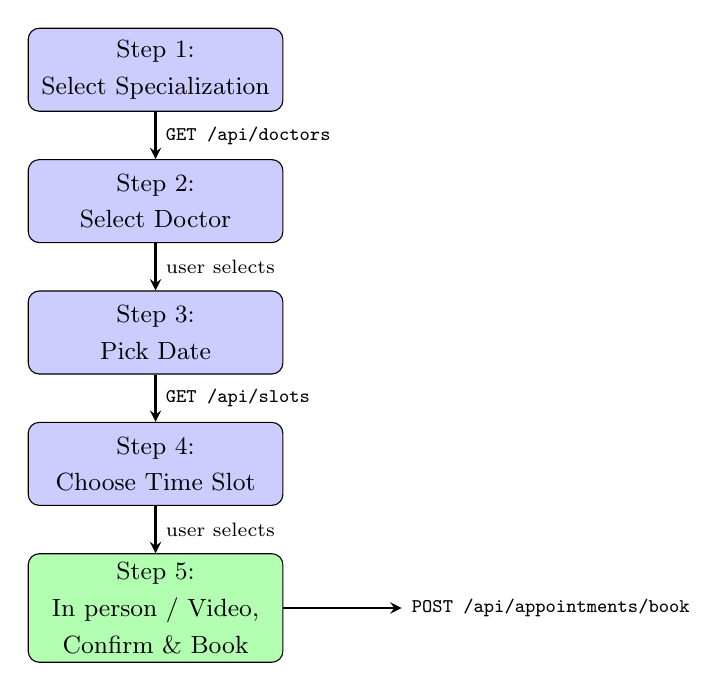
\begin{tikzpicture}[node distance=0.6cm, font=\small]
\node[process, fill=blue!20, text width=3cm] (S1) {Step 1:\\Select Specialization};
\node[process, fill=blue!20, text width=3cm, below=of S1] (S2) {Step 2:\\Select Doctor};
\node[process, fill=blue!20, text width=3cm, below=of S2] (S3) {Step 3:\\Pick Date};
\node[process, fill=blue!20, text width=3cm, below=of S3] (S4) {Step 4:\\Choose Time Slot};
\node[process, fill=green!30, text width=3cm, below=of S4] (S5) {Step 5:\\In person / Video,\\Confirm \& Book};

\draw[arrow] (S1) -- node[right, font=\scriptsize]{\texttt{GET /api/doctors}} (S2);
\draw[arrow] (S2) -- node[right, font=\scriptsize]{user selects} (S3);
\draw[arrow] (S3) -- node[right, font=\scriptsize]{\texttt{GET /api/slots}} (S4);
\draw[arrow] (S4) -- node[right, font=\scriptsize]{user selects} (S5);
\draw[arrow] (S5.east) -- ++(1.5,0) node[right, font=\scriptsize]{\texttt{POST /api/appointments/book}};
\end{tikzpicture}
\caption{Patient Appointment Booking Flow}
\label{fig:bookflow}
\end{figure}

\FloatBarrier
\section{AI Chatbot (MediBot) Implementation}

\FloatBarrier
\subsection{System Prompt Engineering}

In the case of Gemini model, initialization is done using a structure-based system prompt, which provides details regarding the persona of the MediBot, what it can do, the specializations that are available, how to book the session, required output format, and other rules.

\FloatBarrier
\subsection{Action Block Parsing}

After each Gemini API response, the frontend parses for a structured action block at the end of the message text using a regex pattern:

\begin{lstlisting}[language=JavaScript, caption=Action Block Parsing in Chatbot Frontend]
const actionMatch = text.match(/>>>ACTION:(\{.*?\})/s);
if (actionMatch) {
  const action = JSON.parse(actionMatch[1]);
  if (action.type === 'SHOW_DOCTORS') fetchDoctors(action.specialization);
  if (action.type === 'SHOW_APPOINTMENTS') fetchAppointments(action.filter);
  // ... handle other action types
  cleanText = text.replace(/>>>ACTION:.*$/s, '').trim();
}
\end{lstlisting}


\FloatBarrier
\subsection{Safe Rendering of Chatbot Output}

MediBot's replies use a small subset of Markdown (bold text and links), which the widget converts to HTML. In the first version this conversion inserted the model's text into the page without escaping it, so a reply containing HTML, which a user could provoke through prompt injection, would have been executed by the browser (cross-site scripting). The renderer was rewritten as a separate, tested function: it first escapes the five HTML special characters, then converts the Markdown, and only accepts link targets that are absolute \texttt{http(s)} URLs or same-site paths. Protocol-relative targets such as \texttt{//evil.com} and \texttt{/\textbackslash evil.com}, which browsers treat as links to another host, and schemes such as \texttt{javascript:} are left as plain text.

\begin{lstlisting}[language=JavaScript, caption=Escaping Renderer for MediBot Replies (utils/renderMarkdown.ts)]
const SAFE_URL = /^(https?:\/\/|\/(?![/\\]))/i;
export function renderMarkdown(text) {
  return text
    .replace(/[&<>"']/g, (c) => ESCAPES[c])          // escape first
    .replace(/\*\*(.*?)\*\*/g, '<strong>$1</strong>')
    .replace(/\[(.*?)\]\((.*?)\)/g, (m, label, url) =>
      SAFE_URL.test(url) ? `<a href="${url}" ...>${label}</a>` : m)
    .replace(/\n/g, '<br/>');
}
\end{lstlisting}

\FloatBarrier
\section{Security Analysis}
\label{sec:security}

Table~\ref{tab:security} summarizes the security measures implemented in the system. Rows marked (v2) were added or changed in this phase.

\begin{longtable}{|L{3.3cm}|L{10.2cm}|}
\caption{Security Implementation Summary} \label{tab:security} \\
\hline
\textbf{Security Aspect} & \textbf{Implementation} \\
\hline
\endfirsthead
\hline
\textbf{Security Aspect} & \textbf{Implementation} \\
\hline
\endhead
Password Storage & bcryptjs with salt factor 10; plaintext passwords never stored \\
\hline
Authentication (v2) & 15-minute access JWT and 7-day rotating refresh JWT in httpOnly, Secure, SameSite cookies; token type checked \\
\hline
Authorization & Two-layer middleware: JWT verification + role enforcement; multi-role guards; ownership checks return 404 so that other users' records are not revealed; least privilege: doctors request beds, only the admin assigns and discharges \\
\hline
CSRF (v2) & Double-submit token: random readable cookie (lifetime of the refresh cookie) echoed in \texttt{X-CSRF-Token} on every POST/PUT/PATCH/DELETE; failures carry the code \texttt{CSRF\_INVALID} and are retried once by the client; only the HMAC-signed webhook is exempt \\
\hline
Input Validation (v2) & Zod schemas on body, query and params of every route; unknown or malformed input rejected with 400 \\
\hline
Rate Limiting (v2) & Login/register: 10 \emph{failed} attempts per 15 minutes per IP, and login also 10 failures per account e-mail, so password guessing stays limited when attackers rotate IPs; chatbot: 20 messages per minute. \texttt{TRUST\_PROXY\_HOPS=2} behind Vercel and Render, so the limiter sees each visitor's own IP \\
\hline
SQL Injection & Parameterized queries via mysql2 prepared statements throughout; dynamic \texttt{IN} lists built with placeholders \\
\hline
XSS (v2) & React escapes output by default; MediBot Markdown renderer escapes HTML and whitelists link schemes \\
\hline
Payments (v2) & Amount computed on server from doctor's fee; HMAC-SHA256 signature verified with constant-time compare; webhook signed and idempotent; mock mode refused in production \\
\hline
Video Rooms (v2) & 128-bit random room names; only the booked patient and doctor can obtain them; patient must have paid and is admitted by the doctor from a waiting room; time window enforced; on JaaS a 2-hour RS256 token scoped to the room, doctor as moderator, recording disabled \\
\hline
File Upload Safety (v2) & In-memory upload; type detected from the file's first bytes, not its name; 5 MB (prescriptions) and 2 MB (photos) caps; stored in MySQL; prescription files served only to their patient and doctor, with \texttt{nosniff} and \texttt{no-store} \\
\hline
Security Headers (v2) & \texttt{X-Content-Type-Options: nosniff}, \texttt{X-Frame-Options: DENY}, \texttt{Referrer-Policy}, HSTS in production, on the API, Nginx and Vercel; \texttt{X-Powered-By} disabled \\
\hline
CORS Policy & Credentialed requests allowed only from the configured frontend origin \\
\hline
Transport (v2) & HTTPS in production; TLS to the managed database, verified against the provider's CA certificate \\
\hline
Error Exposure & Global error handler returns sanitized messages; stack traces suppressed in production \\
\hline
Double-Booking & UNIQUE constraint on \texttt{active\_slot\_id} + \texttt{FOR UPDATE} transaction lock; same pattern for beds, bed requests and payments; per-patient booking limits stop one account hoarding the schedule \\
\hline
Secrets & All keys in environment variables, never committed; separate test database and \texttt{.env.test}; personal files that had been committed under \texttt{uploads/} were removed from the repository \\
\hline
\end{longtable}

\FloatBarrier
\section{Testing and Validation}

\FloatBarrier
\subsection{Pre-Seeded Test Data}

The database was seeded with 1 Administrator account and 20 Doctor accounts distributed across 5 medical specializations (4 doctors per specialization: Cardiology, Dermatology, General Medicine, Neurology, and Orthopedics). Each doctor's schedule was pre-populated with 15-minute slots for 14 days, providing a realistic test environment. The migrations of the second phase additionally seed three wards with 22 beds (General Ward A: 10 beds, ICU: 6, Emergency Bay: 6) and a three-floor navigation map of 20 locations and 24 connections. Automated tests do not use this data: each test suite creates its own users and records in a separate test database and deletes them afterwards.

\FloatBarrier
\subsection{Functional Test Cases}

Table~\ref{tab:tests} presents the key functional test cases executed during system validation. Test cases T1--T15 come from the first version, where they were executed by hand. T16--T55 cover the new modules and security features; each of them is checked by at least one automated unit, integration, component or end-to-end test (Chapter~\ref{ch:testing}). T41--T55 were added with the bed request workflow, the video waiting room and the fixes of two code audits.

\begin{longtable}{|C{0.8cm}|L{3.9cm}|L{3.4cm}|L{3.5cm}|C{1.2cm}|}
\caption{Functional Test Cases} \label{tab:tests} \\
\hline
\textbf{ID} & \textbf{Test Description} & \textbf{Input} & \textbf{Expected Output} & \textbf{Result} \\
\hline
\endfirsthead
\hline
\textbf{ID} & \textbf{Test} & \textbf{Input} & \textbf{Expected} & \textbf{Result} \\
\hline
\endhead
T1 & Patient registration with valid data & Name, email, password & 201 Created, JWT returned & PASS \\
\hline
T2 & Registration with duplicate email & Existing email & 409 Conflict & PASS \\
\hline
T3 & Login with correct credentials & Email + password & 200 OK, JWT + user object & PASS \\
\hline
T4 & Login with wrong password & Wrong password & 401 Unauthorized & PASS \\
\hline
T5 & Access patient route without token & No Authorization header & 401 Unauthorized & PASS \\
\hline
T6 & Doctor accessing patient route & Doctor JWT & 403 Forbidden & PASS \\
\hline
T7 & Book available slot & Valid doctorId, slotId & 201 Created, appointment record & PASS \\
\hline
T8 & Book already-booked slot & Booked slotId & 409 Conflict & PASS \\
\hline
T9 & Doctor updates appointment to completed & Appointment ID + status & 200 OK & PASS \\
\hline
T10 & Doctor uploads prescription PDF & Multipart file + notes & 201 Created, file saved & PASS \\
\hline
T11 & Patient views medical history & Auth patient & List of prescriptions & PASS \\
\hline
T12 & Admin creates new doctor & Doctor + user data & Doctor account created & PASS \\
\hline
T13 & Admin deletes user & User ID & 200 OK, user removed & PASS \\
\hline
T14 & Chatbot symptom recommendation & ``I have chest pain'' & Cardiology recommendation & PASS \\
\hline
T15 & Cron slot generation (simulated) & Trigger generateSlots() & Slots created for next 14 days & PASS \\
\hline
T16 & Request without CSRF header & POST with session cookie, no X-CSRF-Token & 403 Forbidden & PASS \\
\hline
T17 & Refresh token sent as access token & Cookie with type = refresh & 401, rejected by type check & PASS \\
\hline
T18 & Invalid body & Booking with slotId = "abc" & 400 with field errors & PASS \\
\hline
T19 & Video booking while payments are not configured & consultationType = video & 400, booking refused & PASS \\
\hline
T20 & Record donation within 56 days & Same donor twice & 409 Conflict & PASS \\
\hline
T21 & Fulfil request for B$-$ packed RBC & Stock: B+, B$-$, O$-$, O+ & Only B$-$ then O$-$ units issued, earliest expiry first & PASS \\
\hline
T22 & Fulfil request with too little stock & Need 3, have 2 & 409, no unit issued & PASS \\
\hline
T23 & Allocate occupied bed & Second patient & 409 Bed is not available & PASS \\
\hline
T24 & Admit already-admitted patient & Second bed & 409 Patient already admitted & PASS \\
\hline
T25 & Two concurrent admissions of one patient & Parallel requests & One 201, one 409, no 500 & PASS \\
\hline
T26 & Discharge then re-admit & Allocation id & 200, bed free, re-admit 201 & PASS \\
\hline
T27 & ESI suggestion & 2+ resources, SpO\textsubscript{2} 88\% & Level 2 suggested & PASS \\
\hline
T28 & Emergency queue order & Levels 3, 1, 2 & Ordered 1, 2, 3; level 1 alerts staff & PASS \\
\hline
T29 & Invalid status transition & Reopen a discharged case & 409 Conflict & PASS \\
\hline
T30 & Join unpaid video visit (patient) & In window, unpaid & 402 Payment Required & PASS \\
\hline
T31 & Join outside window & 2 h before start & 403 with start time & PASS \\
\hline
T32 & Join someone else's visit & Other patient & 404 Not Found & PASS \\
\hline
T33 & Shortest route & Main Entrance $\rightarrow$ Neurology & Path with steps and total distance & PASS \\
\hline
T34 & Accessible route & Same, accessible=true & Route uses lifts, no stairs & PASS \\
\hline
T35 & Create payment order & Own unpaid appointment & Amount = doctor fee $\times$ 100 paise & PASS \\
\hline
T36 & Verify with forged signature & Wrong HMAC & 400, appointment stays unpaid & PASS \\
\hline
T37 & Webhook delivered twice & Same event id & Processed once, second is a no-op & PASS \\
\hline
T38 & Pay for past appointment & Started over 60 min ago & 400, Pay button hidden & PASS \\
\hline
T39 & Notifications & Booking made & Patient and doctor each get one; mark-all-read clears count & PASS \\
\hline
T40 & MediBot XSS payload & Reply contains \texttt{<img onerror>} & Rendered as text, no script runs & PASS \\
\hline
T41 & Doctor requests a bed; admin assigns it & Patient, ward type, urgency & Bed allocated, doctor becomes attending doctor, both notified & PASS \\
\hline
T42 & Second pending bed request for the same patient & Duplicate request & 409 Conflict & PASS \\
\hline
T43 & Doctor allocates a bed directly & Doctor session & 403 Forbidden & PASS \\
\hline
T44 & Emergency bed request assigned by admin & ESI case, request-bed & Case status becomes admitted & PASS \\
\hline
T45 & Patient joins a paid video visit before admission & In window, paid & \{waiting: true\}, no room details & PASS \\
\hline
T46 & Doctor admits the waiting patient & POST /admit & Patient's next join returns room and token & PASS \\
\hline
T47 & Stranger opens another patient's prescription file & Other user's session & 404 Not Found & PASS \\
\hline
T48 & Upload a script renamed to .pdf & Wrong file signature & 400, file rejected & PASS \\
\hline
T49 & Doctor cancels a paid visit & Appointment id & Slot free again, payment refund\_due, patient notified & PASS \\
\hline
T50 & Patient cancels a visit that has started & Past start time & 400, not cancelled & PASS \\
\hline
T51 & Delete an appointment that has a payment & Admin delete & 409, payment kept & PASS \\
\hline
T52 & Book a sixth upcoming visit / second visit with same doctor that day & Booking & 409 BOOKING\_LIMIT & PASS \\
\hline
T53 & Book 20 days ahead & Date outside window & 400, no slot rows created & PASS \\
\hline
T54 & Complete a visit 2 hours early & Doctor action & 400, still pending & PASS \\
\hline
T55 & 10 failed logins on one account from 10 IPs; 12 successful logins from one IP & Login requests & 11th attempt on the account returns 429; all 12 successes return 200 & PASS \\
\hline
\end{longtable}

All 40 functional test cases passed, confirming that the system behaves correctly across all core workflows and error conditions.

\FloatBarrier
\subsection{System Workflow Validation}

Figure~\ref{fig:seqdiag} illustrates the sequence of interactions during a complete patient appointment booking session.

\begin{figure}[H]
\centering
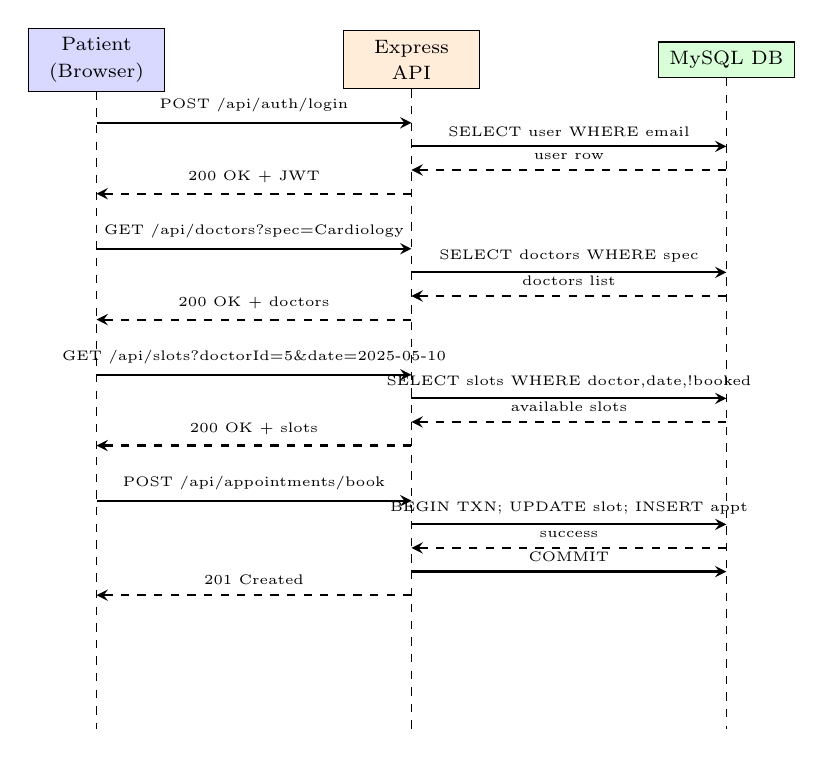
\begin{tikzpicture}[font=\scriptsize, node distance=1cm]

% Lifelines
\node[draw, fill=blue!15, text width=1.5cm, text centered] (P) at (0,0) {Patient (Browser)};
\node[draw, fill=orange!15, text width=1.5cm, text centered] (A) at (4,0) {Express API};
\node[draw, fill=green!15, text width=1.5cm, text centered] (D) at (8,0) {MySQL DB};

\draw[dashed] (P) -- (0,-8.5);
\draw[dashed] (A) -- (4,-8.5);
\draw[dashed] (D) -- (8,-8.5);

% Messages
\draw[arrow] (0,-0.8) -- node[above, font=\tiny]{POST /api/auth/login} (4,-0.8);
\draw[arrow] (4,-1.1) -- node[above, font=\tiny]{SELECT user WHERE email} (8,-1.1);
\draw[arrow, dashed] (8,-1.4) -- node[above, font=\tiny]{user row} (4,-1.4);
\draw[arrow, dashed] (4,-1.7) -- node[above, font=\tiny]{200 OK + JWT} (0,-1.7);

\draw[arrow] (0,-2.4) -- node[above, font=\tiny]{GET /api/doctors?spec=Cardiology} (4,-2.4);
\draw[arrow] (4,-2.7) -- node[above, font=\tiny]{SELECT doctors WHERE spec} (8,-2.7);
\draw[arrow, dashed] (8,-3.0) -- node[above, font=\tiny]{doctors list} (4,-3.0);
\draw[arrow, dashed] (4,-3.3) -- node[above, font=\tiny]{200 OK + doctors} (0,-3.3);

\draw[arrow] (0,-4.0) -- node[above, font=\tiny]{GET /api/slots?doctorId=5\&date=2025-05-10} (4,-4.0);
\draw[arrow] (4,-4.3) -- node[above, font=\tiny]{SELECT slots WHERE doctor,date,!booked} (8,-4.3);
\draw[arrow, dashed] (8,-4.6) -- node[above, font=\tiny]{available slots} (4,-4.6);
\draw[arrow, dashed] (4,-4.9) -- node[above, font=\tiny]{200 OK + slots} (0,-4.9);

\draw[arrow] (0,-5.6) -- node[above, font=\tiny]{POST /api/appointments/book} (4,-5.6);
\draw[arrow] (4,-5.9) -- node[above, font=\tiny]{BEGIN TXN; UPDATE slot; INSERT appt} (8,-5.9);
\draw[arrow, dashed] (8,-6.2) -- node[above, font=\tiny]{success} (4,-6.2);
\draw[arrow] (4,-6.5) -- node[above, font=\tiny]{COMMIT} (8,-6.5);
\draw[arrow, dashed] (4,-6.8) -- node[above, font=\tiny]{201 Created} (0,-6.8);

\end{tikzpicture}
\caption{Sequence Diagram: Patient Appointment Booking}
\label{fig:seqdiag}
\end{figure}

\FloatBarrier
\subsection{Automated Test Results}

Table~\ref{tab:testsummary} summarises the automated test suites. Their design is described in Chapter~\ref{ch:testing}.

\begin{table}[H]
\centering
\caption{Automated Test Suite Summary}
\label{tab:testsummary}
\renewcommand{\arraystretch}{1.25}
\begin{tabular}{|L{3.6cm}|L{3.4cm}|C{1.5cm}|C{1.5cm}|L{3.0cm}|}
\hline
\rowcolor{blue!12}
\textbf{Suite} & \textbf{Tool} & \textbf{Files} & \textbf{Tests} & \textbf{Result} \\
\hline
Backend unit & Jest & 21 & 165 & 165 passed \\
\hline
Backend integration & Jest + Supertest, real MySQL and Redis & 12 & 80 & 80 passed$^{*}$ \\
\hline
Frontend component and contract & Vitest + Testing Library & 19 & 126 & 126 passed \\
\hline
End-to-end & Playwright (Chrome) & 9 & 12 & 12 passed$^{*}$ \\
\hline
\textbf{Total} & & \textbf{61} & \textbf{383} & \\
\hline
\end{tabular}
\\[4pt]
\footnotesize{$^{*}$ These suites need a local MySQL server (and Redis for the cache test); the integration suite also runs in CI against MySQL and Redis service containers.}
\end{table}

\FloatBarrier
\section{System Features Summary}

Table~\ref{tab:features} provides a summary of all implemented features organized by user role.

\begin{table}[H]
\centering
\caption{Feature Summary by User Role}
\label{tab:features}
\begin{tabular}{|L{2cm}|L{11.5cm}|}
\hline
\textbf{Role} & \textbf{Features} \\
\hline
Patient & Registration \& Login; Profile management (name, age, weight, medical history, guardian, address); Specialization-based doctor browsing; Real-time slot selection and appointment booking (in person or video); Appointment history with prescription download; Doctor rating (1--5 stars) for completed visits; AI chatbot (MediBot) access; \textbf{Cancel an upcoming visit (refund flagged if paid); Online payment and payment history; Join video consultation through the waiting room; Notifications} \\
\hline
Doctor & Login; Dashboard with daily stats (total appointments, pending, completed, today's schedule); Appointment list view with patient details; Complete (from 15 minutes before the start) or cancel appointments; Upload prescription (PDF/image) with clinical notes; Create additional availability slots; \textbf{Bed and discharge requests, own patients' beds; Blood stock view and requests; Emergency board (register, triage, treat, request bed); Waiting room: admit the patient, run and complete video consultations; Notifications} \\
\hline
Admin & Login; System dashboard (total users, doctors, appointments, stats); Full CRUD on patient accounts; Full CRUD on doctor accounts (creates linked user + doctor records); Server-side search and paging of users and appointments; Appointment management (view, complete, cancel, delete unless paid); Slot management (view by doctor/date, toggle individual slots, block entire days, manually trigger slot generation); \textbf{Wards and beds; bed and discharge request queue; Blood bank (donors, donations, units, issue/reject requests); Emergency board; Payments ledger with totals and refunds due; Navigation map editing; Notifications} \\
\hline
MediBot & Available to all users (unauthenticated for chat, authenticated for booking); Symptom-to-specialization mapping; Doctor recommendations; Conversational appointment booking through the same endpoint and rules as the booking page; Appointment history retrieval (patients only); replies rendered through an escaping Markdown renderer \\
\hline
Visitor & \textbf{Public hospital navigation with shortest and accessible routes}; doctor and slot browsing; MediBot chat \\
\hline
\end{tabular}
\end{table}


\chapter{Enhanced Hospital Modules}
\label{ch:modules}
\lhead{\emph{Chapter 5: Enhanced Hospital Modules}}
\FloatBarrier
\section{Overview}

This chapter describes the seven modules added in the second phase of the project, together with the doctor-to-administrator request workflow for beds, the video waiting room, and cancellation with refunds, which were added after the first deployment. Each section states the purpose of the module, the workflow it supports, the rules it enforces, and the most important parts of its implementation. All modules share the platform described in Chapters~\ref{ch:design} and~\ref{ch:impl}: the same authentication and role guards, Zod validation, typed errors, the \texttt{inTransaction} helper, and the notification service. The frontend pages for beds, blood bank, emergency and teleconsultation live in a \texttt{shared/} folder because the same page serves both doctors and administrators; the page hides the actions the current role is not allowed to perform, while the server enforces the same rule independently.

\FloatBarrier
\section{Blood Bank Management}
\label{sec:mod-blood}

\subsection{Purpose and Workflow}

The blood bank module replaces the paper register of a hospital blood bank. Administrators register donors and record each donation, which creates a \emph{unit} of a given component (whole blood, packed red cells, plasma or platelets) with a computed expiry date. Doctors and administrators can see the live inventory grouped by blood group and component, and raise a \emph{request} for a patient, with an urgency of routine, urgent or emergency. An administrator then fulfils the request, at which point the system selects and issues the units, or rejects it with a note. The requesting doctor can cancel a request while it is still pending. Figure~\ref{fig:bloodlife} shows the life cycle of a request and of a unit.

\begin{figure}[H]
\centering
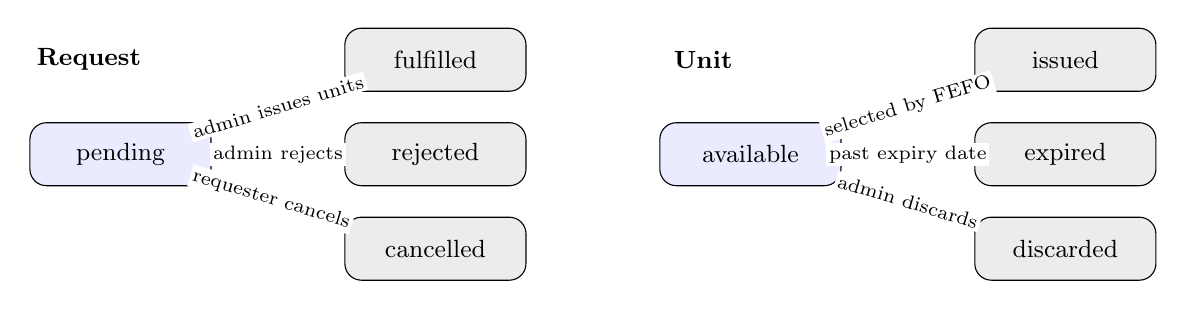
\begin{tikzpicture}[
  st/.style={draw, rounded corners=6pt, minimum width=2.3cm, minimum height=0.8cm, align=center, font=\small, fill=blue!8},
  fin/.style={st, fill=gray!15},
  arr/.style={->, >=stealth, thick},
  lbl/.style={font=\scriptsize, fill=white, inner sep=1pt}
]
\node[font=\bfseries\small] at (-0.4,1.2) {Request};
\node[st] (pend) at (0,0) {pending};
\node[fin] (ful) at (4,1.2) {fulfilled};
\node[fin] (rej) at (4,0) {rejected};
\node[fin] (can) at (4,-1.2) {cancelled};
\draw[arr] (pend) -- node[lbl, sloped]{admin issues units} (ful);
\draw[arr] (pend) -- node[lbl]{admin rejects} (rej);
\draw[arr] (pend) -- node[lbl, sloped, pos=0.45]{requester cancels} (can);

\node[font=\bfseries\small] at (7.4,1.2) {Unit};
\node[st] (av) at (8,0) {available};
\node[fin] (is) at (12,1.2) {issued};
\node[fin] (ex) at (12,0) {expired};
\node[fin] (di) at (12,-1.2) {discarded};
\draw[arr] (av) -- node[lbl, sloped]{selected by FEFO} (is);
\draw[arr] (av) -- node[lbl]{past expiry date} (ex);
\draw[arr] (av) -- node[lbl, sloped]{admin discards} (di);
\end{tikzpicture}
\caption{Life Cycle of a Blood Request and a Blood Unit}
\label{fig:bloodlife}
\end{figure}

\subsection{Business Rules}

\begin{itemize}
    \item \textbf{Compatibility.} Table~\ref{tab:bloodcompat} lists the donor groups that can be issued to each recipient group. Red-cell components use the red-cell ABO table and respect the Rh factor; plasma uses the reversed plasma table and ignores Rh; platelets use the plasma ABO table with the Rh rule \cite{aabb2020}.
    \item \textbf{Exact match first.} Among compatible units, units of the recipient's own group are always issued before substitutes, so that scarce universal-donor O$-$ stock is preserved.
    \item \textbf{First-expiry-first-out (FEFO).} Within the same preference, the unit that expires first is issued first, which minimises wastage.
    \item \textbf{All or nothing.} A request is fulfilled only if enough compatible, unexpired units exist for the full quantity; otherwise nothing is issued and the administrator receives a \texttt{409 Conflict}.
    \item \textbf{Shelf life.} Expiry is computed from the collection date: whole blood 35 days, packed red cells 42 days, plasma 365 days, platelets 5 days. Units past their expiry are marked \texttt{expired} automatically before stock is read or issued.
    \item \textbf{Donor safety.} A donor cannot donate again within 56 days of the previous donation, and a donation date cannot lie in the future \cite{who2012donor}.
    \item \textbf{Alerts.} An emergency-urgency request notifies all administrators, and when an issue leaves fewer than five available units of a group and component, all administrators receive a low-stock alert.
\end{itemize}

\begin{table}[H]
\centering
\caption{Compatible Donor Groups by Recipient and Component (Preferred Order)}
\label{tab:bloodcompat}
\renewcommand{\arraystretch}{1.2}
\begin{tabular}{|C{1.6cm}|L{6.0cm}|L{5.6cm}|}
\hline
\rowcolor{blue!12}
\textbf{Recipient} & \textbf{Whole blood / packed red cells} & \textbf{Plasma} \\
\hline
O$-$  & O$-$ & O$-$, O+, A+, A$-$, B+, B$-$, AB+, AB$-$ \\
\hline
O+    & O+, O$-$ & O+, O$-$, A+, A$-$, B+, B$-$, AB+, AB$-$ \\
\hline
A$-$  & A$-$, O$-$ & A$-$, A+, AB+, AB$-$ \\
\hline
A+    & A+, A$-$, O+, O$-$ & A+, A$-$, AB+, AB$-$ \\
\hline
B$-$  & B$-$, O$-$ & B$-$, B+, AB+, AB$-$ \\
\hline
B+    & B+, B$-$, O+, O$-$ & B+, B$-$, AB+, AB$-$ \\
\hline
AB$-$ & AB$-$, A$-$, B$-$, O$-$ & AB$-$, AB+ \\
\hline
AB+   & AB+, AB$-$, A+, A$-$, B+, B$-$, O+, O$-$ & AB+, AB$-$ \\
\hline
\end{tabular}
\end{table}

\subsection{Implementation}

The compatibility rules are a pure function, \texttt{compatibleDonorGroups(recipient, component)}, which is unit-tested exhaustively for all eight groups and four components. Fulfilment runs inside one transaction: the request row is locked first, expired units are swept, and then the required number of units are selected and locked in a single query whose \texttt{ORDER BY} implements both preferences:

\begin{lstlisting}[language=SQLx, caption=Exact-Group-First FEFO Unit Selection (bloodBankService.js)]
SELECT id FROM blood_units
WHERE status = 'available' AND component = ?
  AND blood_group IN (?)           -- compatible groups only
  AND expires_on >= CURDATE()
ORDER BY (blood_group = ?) DESC,   -- exact match first
         expires_on ASC, id ASC    -- then earliest expiry
LIMIT ? FOR UPDATE
\end{lstlisting}

If fewer rows than requested are returned, the service throws a conflict and the transaction rolls back. Otherwise the units are marked \texttt{issued} with a guarded update (\texttt{WHERE status = 'available'}), the request is marked \texttt{fulfilled}, and after the commit the requesting doctor and the patient are notified. A composite index on \texttt{(status, component, blood\_group, expires\_on)} serves this query. An integration test fires two fulfil requests that compete for the same stock at the same time and checks that exactly one succeeds, one receives \texttt{409}, and neither causes a server error.

\FloatBarrier
\section{Bed Management}
\label{sec:mod-beds}

\subsection{Purpose and Workflow}

Administrators create wards (general, ICU, emergency, maternity, paediatric or private) and beds with a daily rate. The bed board shows every bed with its status (available, occupied, maintenance or reserved) and, for occupied beds, the patient's name and admission time. Each ward card shows total, available and occupied counts, and a statistics panel shows hospital-wide occupancy. Administrators can put a free bed into maintenance or reserve it, but cannot change the status of an occupied bed; an occupied bed becomes free only through discharge. A patient with an open admission cannot be deleted by the administrator.

In a hospital, the decision that a patient needs a bed is clinical, but which bed is free is known to the bed manager. The module follows the same division of work, on the principle of least privilege: \emph{doctors request, the administrator assigns}. Only the administrator can allocate a bed, discharge a patient, or see the full bed grid with patient names. A doctor instead raises a \emph{bed request} for a patient, with a preferred ward type, an urgency (routine, urgent or emergency) and a reason, or a \emph{discharge request} for a patient they admitted. Both kinds of request appear in the administrator's Requests tab, newest emergency first, and inside the Allocate dialog of the bed grid, where requests for the selected bed's ward type are listed first. A bed with a pending discharge request is highlighted in the grid with the requesting doctor, urgency and reason, and its button reads \emph{Approve discharge}. The administrator can also admit a walk-in patient directly from the grid and name an attending doctor.

The doctor whose request led to an admission becomes the \emph{attending doctor} of that stay (\texttt{bed\_allocations.attending\_doctor\_id}). Doctors see only the beds of their own admitted patients, and can request the discharge only of those stays. Figure~\ref{fig:bedreq} shows the life cycle of a request; every change notifies the people involved (Table~\ref{tab:notiftypes}).

\begin{figure}[H]
\centering
\resizebox{\textwidth}{!}{%
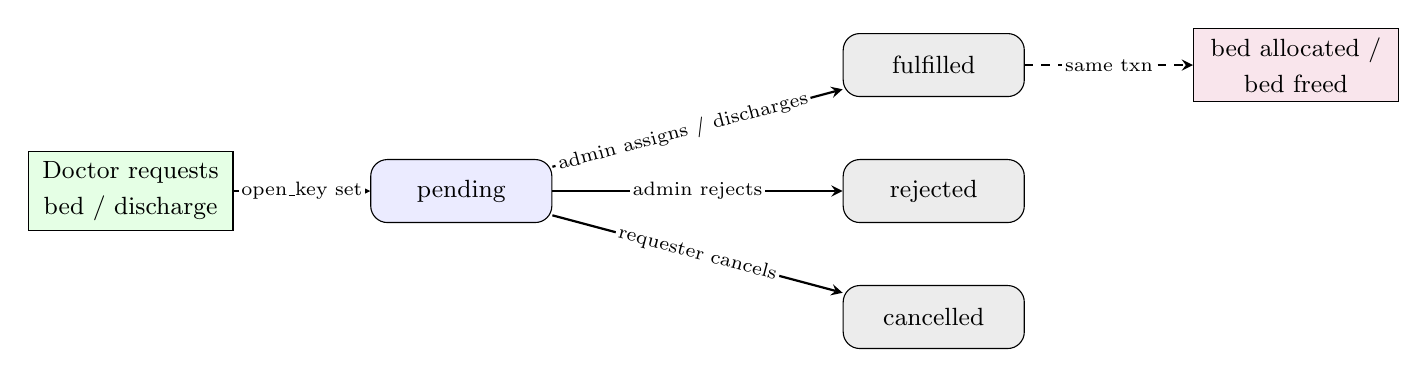
\begin{tikzpicture}[
  st/.style={draw, rounded corners=6pt, minimum width=2.3cm, minimum height=0.8cm, align=center, font=\small, fill=blue!8},
  fin/.style={st, fill=gray!15},
  act/.style={draw, minimum width=2.6cm, minimum height=0.8cm, align=center, font=\small, fill=green!10},
  arr/.style={->, >=stealth, thick},
  lbl/.style={font=\scriptsize, fill=white, inner sep=1pt}
]
\node[act] (doc) at (-4.2,0) {Doctor requests\\bed / discharge};
\node[st] (pend) at (0,0) {pending};
\node[fin] (ful) at (6.0,1.6) {fulfilled};
\node[fin] (rej) at (6.0,0) {rejected};
\node[fin] (can) at (6.0,-1.6) {cancelled};
\node[act, fill=purple!10] (eff) at (10.6,1.6) {bed allocated /\\bed freed};
\draw[arr] (doc) -- node[lbl]{open\_key set} (pend);
\draw[arr] (pend) -- node[lbl, sloped, pos=0.45]{admin assigns / discharges} (ful);
\draw[arr] (pend) -- node[lbl]{admin rejects} (rej);
\draw[arr] (pend) -- node[lbl, sloped]{requester cancels} (can);
\draw[arr, dashed] (ful) -- node[lbl]{same txn} (eff);
\end{tikzpicture}%
}
\caption{Life Cycle of a Bed or Discharge Request}
\label{fig:bedreq}
\end{figure}

\subsection{One Pending Request at a Time}

A patient may have at most one pending admission request, and an admission at most one pending discharge request. As with allocations, the rule is enforced by a unique key rather than by a check alone: \texttt{bed\_requests.open\_key} holds \texttt{admission:<patient id>} or \texttt{discharge:<allocation id>} while the request is pending and is set to \texttt{NULL} when it is fulfilled, rejected or cancelled. A duplicate request therefore fails with \texttt{ER\_DUP\_ENTRY}, which the service turns into a \texttt{409 Conflict}. Assigning a bed for a request locks the request, then the linked emergency case if there is one, and then follows the bed service's lock order (bed, patient, allocation). Assigning from the grid for a patient who has a pending request goes through the same code, so the request is always marked fulfilled and an emergency case is always marked admitted, whichever screen the administrator uses. One subtle point was found by a concurrency test: looking up a missing pending request with \texttt{SELECT \ldots{} FOR UPDATE} on the unique key takes an InnoDB \emph{gap lock} that deadlocks with a doctor's concurrent \texttt{INSERT}. The service therefore reads the key without a lock first and locks the row by its primary key only if it exists.

\subsection{Preventing Double Allocation}

The central correctness requirement is that a bed never has two open allocations and a patient is never admitted to two beds. The application checks both conditions inside a transaction that locks the bed row and the patient's user row (in that fixed order), but application checks alone are not a complete defence: a future code path, a manual SQL statement, or an unforeseen race could still insert a second open row. The guarantee is therefore moved into the schema.

MySQL cannot express ``unique where \texttt{discharged\_at IS NULL}'' directly, and MySQL~8 also forbids a stored generated column over a column that has a cascading foreign key, which rules out the usual computed-column trick. Instead, \texttt{bed\_allocations} has two plain columns, \texttt{open\_bed\_id} and \texttt{open\_patient\_id}, each with a \texttt{UNIQUE} index. They hold the bed and patient ids while the stay is open and are set to \texttt{NULL} on discharge. Because a unique index allows any number of \texttt{NULL} values, closed stays never conflict, while a second open stay for the same bed or patient is rejected by the database itself:

\begin{lstlisting}[language=JavaScript, caption=Allocation Insert Backed by Unique Keys (bedService.js)]
try {
  [ins] = await conn.query(
    `INSERT INTO bed_allocations (bed_id, patient_id, allocated_by,
        attending_doctor_id, reason, open_patient_id, open_bed_id)
     VALUES (?, ?, ?, ?, ?, ?, ?)`,
    [bedId, patientId, allocatedBy ?? null, attending,
     reason ?? request?.reason ?? null, patientId, bedId]);
} catch (err) {
  if (err.code !== 'ER_DUP_ENTRY') throw err;
  throw new ConflictError(/uq_alloc_open_bed/.test(err.message)
    ? 'Bed is not available.' : 'Patient already admitted.');
}
// discharge: SET discharged_at = NOW(), open_patient_id = NULL, open_bed_id = NULL
\end{lstlisting}

The bed's status is then flipped with a guarded update (\texttt{SET status = 'occupied' WHERE id = ? AND status = 'available'}), which can never silently overwrite another state. The migration back-fills the two columns for existing open stays before creating the indexes. Tests check the friendly error messages, a concurrent double admission (one \texttt{201}, one \texttt{409}), and that raw duplicate \texttt{INSERT} statements that bypass the application are rejected by MySQL.

\FloatBarrier
\section{Emergency Management and Triage}
\label{sec:mod-emergency}

\subsection{Purpose and Workflow}

The emergency board is used by doctors and administrators in the emergency department. A new arrival is registered with the patient's name (or linked to an existing registered patient), age, gender, contact, chief complaint, arrival mode (walk-in, ambulance or referral) and vital signs (heart rate, respiratory rate, blood pressure, SpO\textsubscript{2}, temperature). While the form is being filled, the ESI algorithm suggests a triage level, which the clinician can accept or override. The open queue is ordered by triage level and then by arrival time, so that a level 1 patient who arrives last is shown first. Each card can be assigned to a doctor (who is notified), moved into treatment, discharged or transferred. When a registered patient needs admission, the doctor presses \emph{Request bed}, which raises a bed request with emergency urgency and notifies the administrators; the administrator assigns the bed, which admits the case. Only the administrator can admit a case directly into a free bed.

\subsection{ESI Triage Algorithm}

The suggestion follows the ESI version 4 decision points \cite{gilboy2012esi}, shown in Figure~\ref{fig:esi}. It is implemented as a pure function in the backend and duplicated in the frontend for instant feedback; both copies are unit-tested against the same cases.

\begin{figure}[H]
\centering
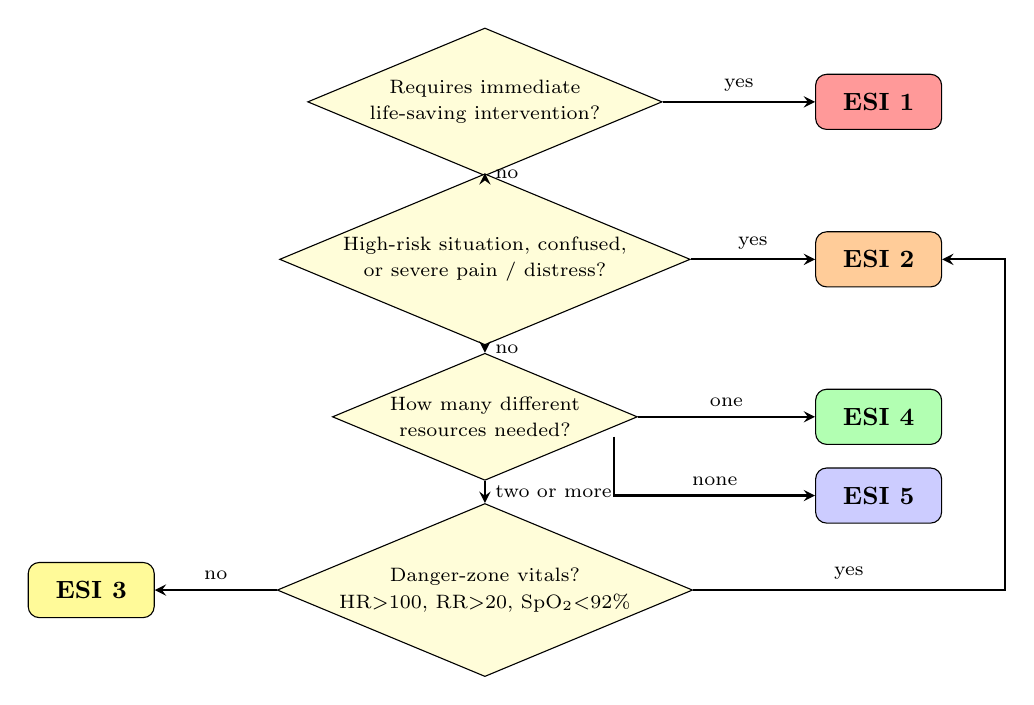
\begin{tikzpicture}[
  q/.style={diamond, draw, aspect=2.4, align=center, font=\scriptsize, fill=yellow!15, inner sep=1pt},
  l/.style={draw, rounded corners, minimum width=1.6cm, minimum height=0.7cm, font=\small\bfseries, align=center},
  arr/.style={->, >=stealth, thick},
  lbl/.style={font=\scriptsize}
]
\node[q] (a) at (0,0) {Requires immediate\\life-saving intervention?};
\node[q] (b) at (0,-2.0) {High-risk situation, confused,\\or severe pain / distress?};
\node[q] (c) at (0,-4.0) {How many different\\resources needed?};
\node[q] (d) at (0,-6.2) {Danger-zone vitals?\\HR$>$100, RR$>$20, SpO\textsubscript{2}$<$92\%};
\node[l, fill=red!40] (l1) at (5,0) {ESI 1};
\node[l, fill=orange!40] (l2) at (5,-2.0) {ESI 2};
\node[l, fill=yellow!40] (l3) at (-5,-6.2) {ESI 3};
\node[l, fill=green!30] (l4) at (5,-4.0) {ESI 4};
\node[l, fill=blue!20] (l5) at (5,-5.0) {ESI 5};
\draw[arr] (a) -- node[lbl, above]{yes} (l1);
\draw[arr] (a) -- node[lbl, right]{no} (b);
\draw[arr] (b) -- node[lbl, above]{yes} (l2);
\draw[arr] (b) -- node[lbl, right]{no} (c);
\draw[arr] (c) -- node[lbl, above]{one} (l4);
\draw[arr] (c.east) ++(-0.3,-0.25) |- node[lbl, pos=0.75, above]{none} (l5.west);
\draw[arr] (c) -- node[lbl, right]{two or more} (d);
\draw[arr] (d) -- node[lbl, above]{no} (l3);
\draw[arr] (d.east) -- node[lbl, above]{yes} (6.6,-6.2) -- (6.6,-2.0) -- (l2.east);
\end{tikzpicture}
\caption{ESI Version 4 Triage Decision Flow Used for the Suggested Level}
\label{fig:esi}
\end{figure}

\subsection{Status Transitions and Admission}

A case moves through a small state machine (Figure~\ref{fig:erstates}). Only the transitions shown are accepted; any other request, such as reopening a discharged case, returns \texttt{409}. The \texttt{admitted} state cannot be set through the generic update endpoint. It is reached in one of two ways, both inside one transaction that calls the same \texttt{allocateBed} service used by the bed board (so the same lock order and unique keys apply), stores the allocation id on the case and closes it: the administrator's direct admit action, or the administrator assigning a bed for the doctor's emergency bed request. If the case is discharged or transferred while its bed request is still pending, the request is cancelled in the same transaction, and assigning a bed for a request whose case is already closed is refused with \texttt{409}. Registering a case with level 1 or 2 notifies every doctor and administrator.

\begin{figure}[H]
\centering
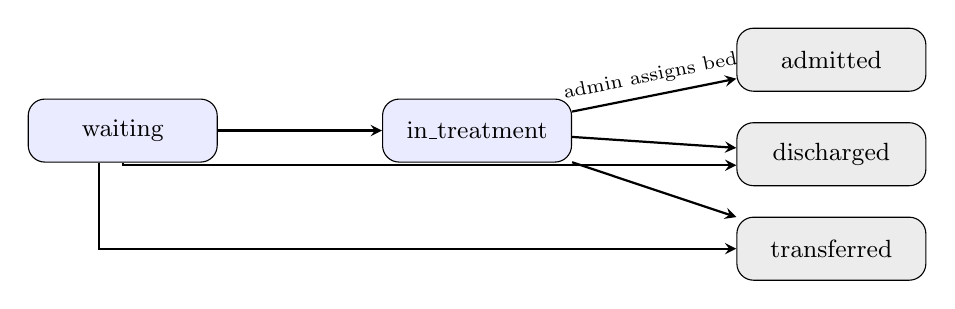
\begin{tikzpicture}[
  st/.style={draw, rounded corners=6pt, minimum width=2.4cm, minimum height=0.8cm, align=center, font=\small, fill=blue!8},
  fin/.style={st, fill=gray!15},
  arr/.style={->, >=stealth, thick}
]
\node[st] (w) at (0,0) {waiting};
\node[st] (t) at (4.5,0) {in\_treatment};
\node[fin] (a) at (9,0.9) {admitted};
\node[fin] (d) at (9,-0.3) {discharged};
\node[fin] (x) at (9,-1.5) {transferred};
\draw[arr] (w) -- (t);
\draw[arr] (t) -- node[font=\scriptsize, above, sloped]{admin assigns bed} (a);
\draw[arr] (t) -- (d);
\draw[arr] (t) -- (x);
\draw[arr] (w.south) |- ([yshift=-4pt]d.west);
\draw[arr] (w.south) ++(-0.3,0) |- (x.west);
\end{tikzpicture}
\caption{Emergency Case Status Transitions}
\label{fig:erstates}
\end{figure}

\FloatBarrier
\section{Teleconsultation}
\label{sec:mod-tele}

\subsection{Purpose and Workflow}

When booking, a patient can choose a video consultation instead of an in-person visit. Video visits require online payment, so they can be booked only when payments are configured. At booking time the server generates a room name of the form \texttt{hms-} followed by 32 random hexadecimal characters (128 bits of randomness), stored in a unique column. At the time of the appointment, the patient and the doctor each open the consultation from their appointment list. The page calls \texttt{GET /api/teleconsult/:appointmentId/join}. The doctor enters the room straight away; the patient enters a \emph{waiting room} instead, as in a real clinic, and is let in only when the doctor clicks \emph{Admit}. After the call, the doctor marks the consultation completed, and the patient is notified.

\subsection{Waiting Room}

Figure~\ref{fig:waitroom} shows the protocol. While the patient waits, the page repeats the join request every five seconds, and each request records the time in \texttt{appointments.video\_waiting\_at}. The doctor's page polls \texttt{GET /status}, which reports the patient as waiting if the last poll was less than 20 seconds ago, so a patient who closed the tab is not shown as waiting. \texttt{POST /admit} sets \texttt{video\_admitted\_at} once; from then on the patient's next join request returns the room details. All three endpoints run the same access checks, and \texttt{/status} and \texttt{/admit} are answered with \texttt{404} for anyone but the appointment's doctor.

\begin{figure}[H]
\centering
\resizebox{\textwidth}{!}{%
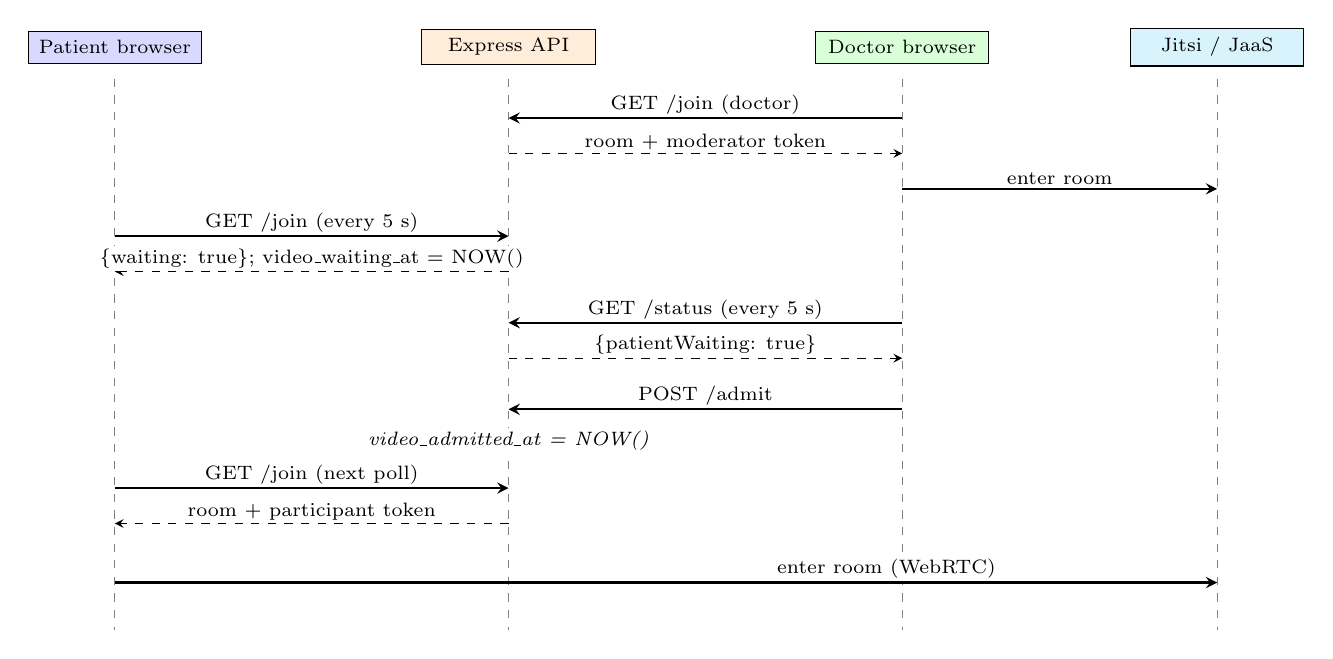
\begin{tikzpicture}[font=\scriptsize, arr/.style={->, >=stealth, thick}, ret/.style={->, >=stealth, dashed}, lb/.style={fill=white, inner sep=1pt}]
\node[draw, fill=blue!15, minimum width=2.2cm] (P) at (0,0) {Patient browser};
\node[draw, fill=orange!15, minimum width=2.2cm] (A) at (5,0) {Express API};
\node[draw, fill=green!15, minimum width=2.2cm] (D) at (10,0) {Doctor browser};
\node[draw, fill=cyan!15, minimum width=2.2cm] (J) at (14,0) {Jitsi / JaaS};
\foreach \x in {0,5,10,14} \draw[dashed, gray] (\x,-0.4) -- (\x,-7.4);
\draw[arr] (10,-0.9) -- node[above, lb]{GET /join (doctor)} (5,-0.9);
\draw[ret] (5,-1.35) -- node[above, lb]{room + moderator token} (10,-1.35);
\draw[arr] (10,-1.8) -- node[above, lb]{enter room} (14,-1.8);
\draw[arr] (0,-2.4) -- node[above, lb]{GET /join (every 5 s)} (5,-2.4);
\draw[ret] (5,-2.85) -- node[above, lb]{\{waiting: true\}; video\_waiting\_at = NOW()} (0,-2.85);
\draw[arr] (10,-3.5) -- node[above, lb]{GET /status (every 5 s)} (5,-3.5);
\draw[ret] (5,-3.95) -- node[above, lb]{\{patientWaiting: true\}} (10,-3.95);
\draw[arr] (10,-4.6) -- node[above, lb]{POST /admit} (5,-4.6);
\node[lb, font=\scriptsize\itshape] at (5,-5.0) {video\_admitted\_at = NOW()};
\draw[arr] (0,-5.6) -- node[above, lb]{GET /join (next poll)} (5,-5.6);
\draw[ret] (5,-6.05) -- node[above, lb]{room + participant token} (0,-6.05);
\draw[arr] (0,-6.8) -- node[above, pos=0.7, lb]{enter room (WebRTC)} (14,-6.8);
\end{tikzpicture}%
}
\caption{Sequence Diagram: Video Waiting Room and Admission by the Doctor}
\label{fig:waitroom}
\end{figure}

\subsection{Access Rules}

Every teleconsultation endpoint applies five checks in order:
\begin{enumerate}
    \item The caller must be the patient who booked the appointment or the doctor assigned to it. Anyone else receives \texttt{404}, so the endpoint does not reveal whether the appointment exists.
    \item The appointment must be a video consultation with a room.
    \item It must still be pending (not completed or cancelled), otherwise \texttt{409}.
    \item A patient must have paid (\texttt{402 Payment Required}); the doctor is not subject to this check.
    \item The current time must be within the join window, from 15 minutes before the start until 60 minutes after it. Outside it the server returns \texttt{403} with the scheduled start time, which the page shows to the user.
\end{enumerate}

The window boundaries are named constants shared with the payment module: a patient can still pay up to 60 minutes after the start, which is exactly as long as the room stays joinable, so a patient is never asked to pay for a consultation they can no longer join.

\subsection{Video Provider and Signed Room Tokens}

During deployment it was found that the public \texttt{meet.jit.si} service no longer allows its rooms to be embedded in third-party websites. The system therefore supports Jitsi as a Service (JaaS, hosted by 8x8 on \texttt{8x8.vc}). When the three variables \texttt{JAAS\_APP\_ID}, \texttt{JAAS\_KID} and \texttt{JAAS\_PRIVATE\_KEY} are set, the join response contains a JSON Web Token signed by the server with the hospital's private key (RS256), valid for two hours and only for that appointment's room. The doctor's token marks them as moderator; recording, live-streaming, transcription and outbound calls are switched off in the token. A person who learns the room name still cannot join without a token, which only the API issues, and only after the checks above. Without the JaaS keys the system falls back to \texttt{JITSI\_DOMAIN}, which is useful for local testing.

\begin{lstlisting}[language=JavaScript, caption=Room-Scoped JaaS Token (utils/videoAccess.js)]
const token = jwt.sign({
  aud: 'jitsi', iss: 'chat', sub: jaas.appId, room, nbf: now - 10,
  context: {
    user: { id: String(user.id), name: user.name, email: user.email,
            moderator: isModerator ? 'true' : 'false' },
    features: { livestreaming: false, recording: false,
                transcription: false, 'outbound-call': false },
  },
}, jaas.privateKey, { algorithm: 'RS256', keyid: jaas.kid, expiresIn: '2h' });
return { domain: '8x8.vc', roomName: `${jaas.appId}/${room}`, jwt: token };
\end{lstlisting}

\FloatBarrier
\section{Notifications and Alerts}
\label{sec:mod-notif}

Notifications are stored in the database and shown through a bell icon in the navigation bar of every signed-in user. The bell shows the unread count, opens a list of the newest notifications, and lets the user open the linked page, mark one notification as read, or mark all as read. The list endpoint supports a limit and an unread-only filter, and is backed by an index on \texttt{(user\_id, is\_read, created\_at)}. A user can only read and update their own notifications; another user's notification id returns \texttt{404}. Table~\ref{tab:notiftypes} lists the events that generate notifications.

\begin{table}[H]
\centering
\caption{Events that Generate Notifications}
\label{tab:notiftypes}
\renewcommand{\arraystretch}{1.2}
\begin{tabular}{|L{2.4cm}|L{5.8cm}|L{5.3cm}|}
\hline
\rowcolor{blue!12}
\textbf{Type} & \textbf{Event} & \textbf{Recipients} \\
\hline
appointment & Appointment booked (form or MediBot) & Patient and doctor \\
\hline
appointment & Appointment cancelled (with refund note if paid) & The other side: doctor if the patient cancelled, patient if the doctor or hospital did, both if the admin did \\
\hline
payment & Payment captured & Patient and doctor \\
\hline
teleconsult & Video consultation completed & Patient \\
\hline
bed & Bed or discharge request raised (doctor or emergency board) & All admins \\
\hline
bed & Request fulfilled (bed assigned or patient discharged) or rejected & Requesting doctor; the patient on admission and discharge \\
\hline
bed & Walk-in admission with a named attending doctor & Patient and attending doctor \\
\hline
emergency & New case with ESI level 1 or 2; case assigned to a doctor & All doctors and admins; assigned doctor \\
\hline
blood & Emergency-urgency request raised; stock of a group/component falls below five units after an issue; request fulfilled & All admins; all admins; requesting doctor and patient \\
\hline
\end{tabular}
\end{table}

As explained in Chapter~\ref{ch:design}, notifications are written after the business transaction commits and their failures are logged, never propagated. Delivery is in-app only; e-mail, SMS and push delivery are listed as future work.

\FloatBarrier
\section{Hospital Navigation}
\label{sec:mod-nav}

\subsection{Purpose and Data Model}

The navigation page is public: a visitor selects a starting point and a destination, optionally ticks ``step-free route'', and receives turn-by-turn directions with the total walking distance and the floor of each step. The hospital is modelled as an undirected weighted graph. Locations (\texttt{nav\_locations}) are nodes with a category, building and floor; connections (\texttt{nav\_edges}) are edges with a distance in metres, a forward and a reverse walking instruction, and an \texttt{accessible} flag that is 0 for staircases. The seeded map covers three floors with 20 locations (entrance, reception, emergency, pharmacy, radiology, lifts, stairs, clinics, wards, blood bank and ICU) and 24 connections. Administrators can add and remove locations and connections.

\subsection{Shortest-Path Algorithm}

For each query the edges are loaded and an adjacency list is built in which every edge is added in both directions with the instruction for that direction. In step-free mode, inaccessible edges are skipped while building the graph, so the search simply cannot use stairs. The route is computed with Dijkstra's algorithm \cite{dijkstra1959}:

\begin{lstlisting}[language=JavaScript, caption=Dijkstra's Algorithm for Indoor Routing (utils/pathfinding.js)]
function shortestPath(graph, fromId, toId) {
  const dist = new Map([[fromId, 0]]), prev = new Map(), done = new Set();
  for (;;) {
    let cur = null;                              // closest unvisited node
    for (const [id, d] of dist)
      if (!done.has(id) && (cur === null || d < dist.get(cur))) cur = id;
    if (cur === null) return null;               // destination unreachable
    if (cur === toId) break;
    done.add(cur);
    for (const e of graph.get(cur) || []) {      // relax neighbours
      const nd = dist.get(cur) + e.distance;
      if (!dist.has(e.to) || nd < dist.get(e.to)) {
        dist.set(e.to, nd);
        prev.set(e.to, { from: cur, instruction: e.instruction, distance: e.distance });
      }
    }
  }
  // walk prev[] back from toId to build the ordered list of steps
}
\end{lstlisting}

The priority queue is a linear scan, giving $O(V^2 + E)$ time. For a hospital map of a few hundred nodes this takes well under a millisecond and avoids extra code; the comment in the source records that a binary heap ($O((V+E)\log V)$) should replace it if the map grows to thousands of nodes. If no route exists (for example a step-free route to a floor with no lift), the API returns \texttt{404} with a clear message rather than an empty list. Unit tests cover shortest-path choice, direction-specific instructions, unreachable targets, the same start and end, and that step-free mode avoids stairs; an end-to-end test drives the public page from Main Entrance to Neurology in both modes.

\FloatBarrier
\section{Online Payments}
\label{sec:mod-payments}

\subsection{Payment Flow}

Patients pay the consultation fee from their appointment history. Figure~\ref{fig:payseq} shows the flow with the Razorpay gateway \cite{razorpaydocs}.

\begin{figure}[H]
\centering
\resizebox{\textwidth}{!}{%
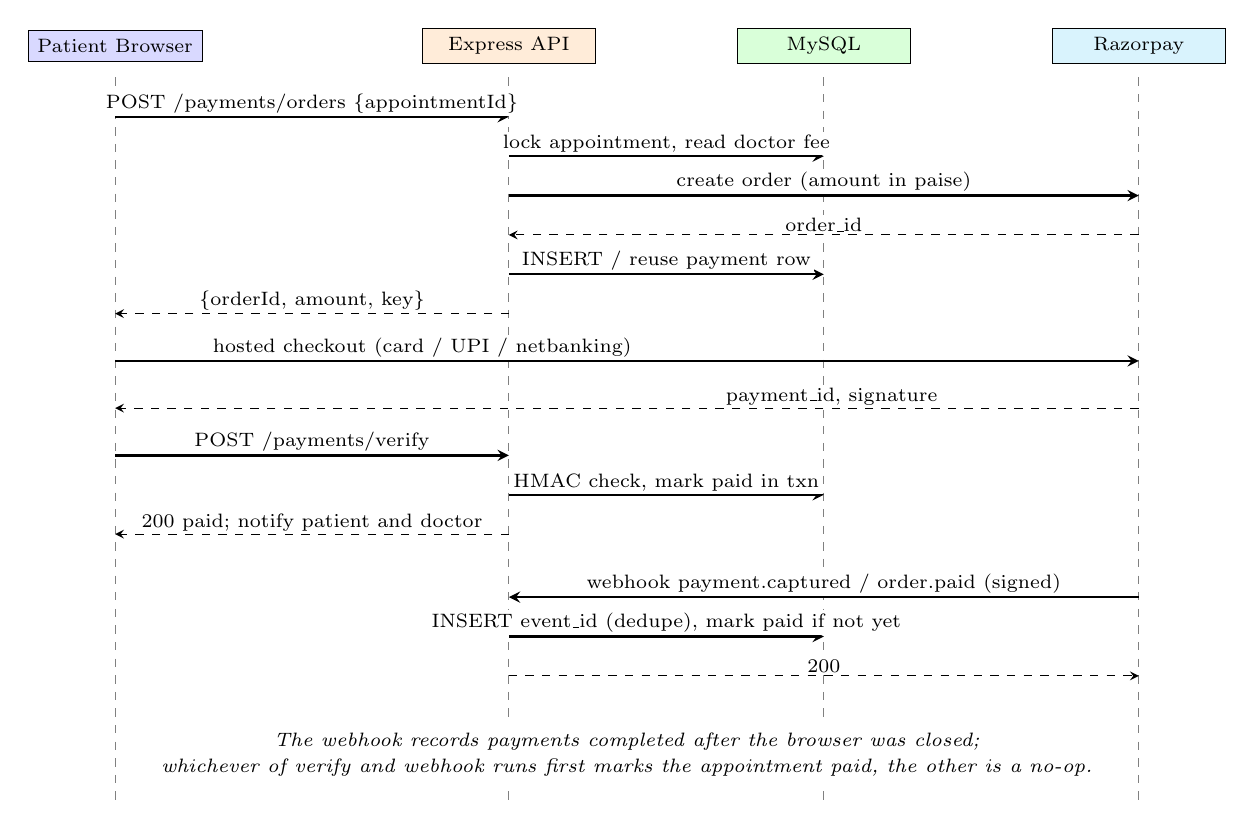
\begin{tikzpicture}[font=\scriptsize, arr/.style={->, >=stealth, thick}, ret/.style={->, >=stealth, dashed}, every label/.style={fill=white}, lb/.style={fill=white, inner sep=1pt}]
\node[draw, fill=blue!15, minimum width=2.2cm, align=center] (B) at (0,0) {Patient Browser};
\node[draw, fill=orange!15, minimum width=2.2cm, align=center] (A) at (5,0) {Express API};
\node[draw, fill=green!15, minimum width=2.2cm, align=center] (D) at (9,0) {MySQL};
\node[draw, fill=cyan!15, minimum width=2.2cm, align=center] (R) at (13,0) {Razorpay};
\foreach \x in {0,5,9,13} \draw[dashed, gray] (\x,-0.4) -- (\x,-9.6);
\draw[arr] (0,-0.9) -- node[above, lb]{POST /payments/orders \{appointmentId\}} (5,-0.9);
\draw[arr] (5,-1.4) -- node[above, lb]{lock appointment, read doctor fee} (9,-1.4);
\draw[arr] (5,-1.9) -- node[above, lb]{create order (amount in paise)} (13,-1.9);
\draw[ret] (13,-2.4) -- node[above, lb]{order\_id} (5,-2.4);
\draw[arr] (5,-2.9) -- node[above, lb]{INSERT / reuse payment row} (9,-2.9);
\draw[ret] (5,-3.4) -- node[above, lb]{\{orderId, amount, key\}} (0,-3.4);
\draw[arr] (0,-4.0) -- node[above, pos=0.3, lb]{hosted checkout (card / UPI / netbanking)} (13,-4.0);
\draw[ret] (13,-4.6) -- node[above, pos=0.3, lb]{payment\_id, signature} (0,-4.6);
\draw[arr] (0,-5.2) -- node[above, lb]{POST /payments/verify} (5,-5.2);
\draw[arr] (5,-5.7) -- node[above, lb]{HMAC check, mark paid in txn} (9,-5.7);
\draw[ret] (5,-6.2) -- node[above, lb]{200 paid; notify patient and doctor} (0,-6.2);
\draw[arr] (13,-7.0) -- node[above, lb]{webhook payment.captured / order.paid (signed)} (5,-7.0);
\draw[arr] (5,-7.5) -- node[above, lb]{INSERT event\_id (dedupe), mark paid if not yet} (9,-7.5);
\draw[ret] (5,-8.0) -- node[above, lb]{200} (13,-8.0);
\node[font=\scriptsize\itshape, align=center, fill=white] at (6.5,-9.0) {The webhook records payments completed after the browser was closed;\\whichever of verify and webhook runs first marks the appointment paid, the other is a no-op.};
\end{tikzpicture}%
}
\caption{Sequence Diagram: Online Payment with Server-Side Verification and Webhook}
\label{fig:payseq}
\end{figure}

\subsection{Security and Correctness Rules}

\begin{itemize}
    \item \textbf{The amount comes from the server.} The client sends only the appointment id; the amount is the doctor's fee converted to paise and read from the database, so it cannot be tampered with.
    \item \textbf{Only payable appointments.} The appointment must belong to the caller, be pending, be unpaid, have a non-zero fee, and not lie more than 60 minutes in the past. The appointment list exposes the same condition as a \texttt{can\_pay} flag computed in SQL, so the \emph{Pay} button is shown exactly when the server would accept the order.
    \item \textbf{Signature verification.} The checkout result is accepted only if \texttt{HMAC-SHA256(key\_secret, order\_id + "|" + payment\_id)} equals the returned signature, compared in constant time to prevent timing attacks. A wrong signature changes nothing.
    \item \textbf{Signed, idempotent webhooks.} The webhook body is verified with the separate webhook secret over the raw request bytes, so the JSON parser is bypassed for this one route. Its event id is inserted into \texttt{payment\_webhook\_events}, whose unique key makes a duplicate delivery a no-op. The webhook is the only state-changing endpoint exempt from CSRF, because it carries no cookies and is authenticated by its signature.
    \item \textbf{Order reuse.} Repeated clicks reuse the existing order while the amount and mode are unchanged, so a patient cannot accumulate several open orders for one appointment.
    \item \textbf{Failing closed.} When Razorpay keys are set, the real gateway is used. Without keys, a mock gateway (with a public test secret) is available only in development and test or with an explicit \texttt{PAYMENT\_MODE=mock}; in production without keys payment returns \texttt{503 Not Configured} rather than silently accepting mock payments.
    \item \textbf{Reconciliation logging.} Rare gateway edge cases, such as a capture on an order that was later replaced, are applied safely and logged with a \texttt{RECONCILE} tag for manual review.
\end{itemize}

\begin{lstlisting}[language=JavaScript, caption=Constant-Time Signature Verification (paymentGateway.js)]
const hmacHex = (secret, data) =>
  crypto.createHmac('sha256', secret).update(data).digest('hex');
function safeEqual(expected, given) {          // never throws
  if (typeof given !== 'string') return false;
  const a = Buffer.from(expected, 'utf8'), b = Buffer.from(given, 'utf8');
  return a.length === b.length && crypto.timingSafeEqual(a, b);
}
function verifyCheckoutSignature(orderId, paymentId, signature) {
  const secret = keySecret();                  // null if payments not configured
  if (!secret || typeof orderId !== 'string' || typeof paymentId !== 'string') return false;
  return safeEqual(hmacHex(secret, `${orderId}|${paymentId}`), signature);
}
\end{lstlisting}

\subsection{Cancellation and Refunds}

Patients, doctors and administrators cancel appointments through one shared service function, so the same rules apply wherever the button is pressed. A patient can cancel only before the start time. Cancelling locks the appointment and then its slot, sets the status to \texttt{cancelled}, clears \texttt{active\_slot\_id} and frees the slot, so that another patient can book it. If the visit was paid, its payment becomes \texttt{refund\_due} and appears in the administrator's ledger; the refund itself is issued from the Razorpay dashboard. If a checkout is still open, its payment row is marked \texttt{failed}, so that a late capture cannot mark a cancelled visit paid; a capture that still arrives for a cancelled visit is stored as \texttt{refund\_due} and logged for reconciliation. After the commit the cached slot list is invalidated and the other side is notified. Payment records also block deletion: the foreign keys from \texttt{payments} to \texttt{appointments} and \texttt{users} are \texttt{ON DELETE RESTRICT}, and the administrator receives a clear \texttt{409} instead of a silent loss of financial history.

\subsection{Payment Views}

Patients see their payment history with status (created, paid, failed or refund due), amount, provider and order/payment ids. Administrators see a ledger of all payments, paginated 50 per page by default (the page size is validated between 1 and 100), together with the total amount collected, the number of paid and pending payments, and the overall count, which drives the page navigation.


\chapter{Testing and Quality Assurance}
\label{ch:testing}
\lhead{\emph{Chapter 6: Testing and Quality Assurance}}
\FloatBarrier
\section{Testing Strategy}

The first version was validated with 15 manual functional tests. As the system grew to fourteen route modules and twenty-one tables, manual testing could no longer give confidence that a change in one module did not break another. The second phase therefore introduced an automated test suite organised as a test pyramid \cite{cohn2009} (Figure~\ref{fig:pyramid}): many fast unit tests for business rules, a smaller number of integration tests that exercise real HTTP routes against a real MySQL database, component tests for the user interface, and a few end-to-end tests that drive a real browser through complete user journeys.

\begin{figure}[H]
\centering
\resizebox{\textwidth}{!}{%
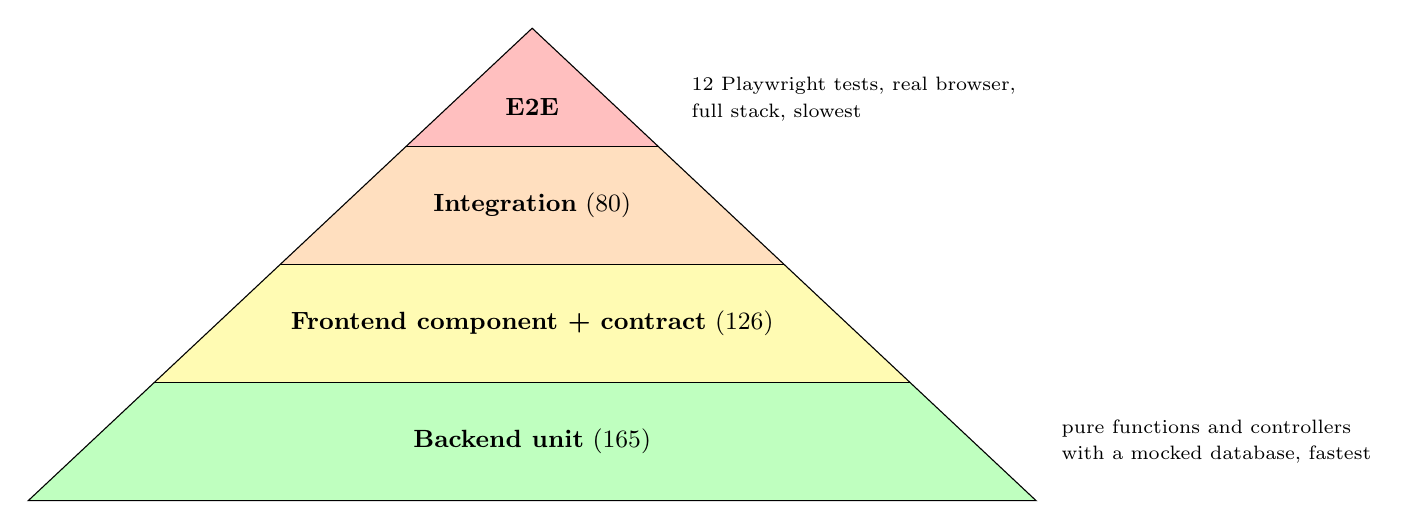
\begin{tikzpicture}[font=\small]
\fill[red!25]    (-1.6,4.5) -- (1.6,4.5) -- (0,6.0) -- cycle;
\fill[orange!25] (-3.2,3.0) -- (3.2,3.0) -- (1.6,4.5) -- (-1.6,4.5) -- cycle;
\fill[yellow!30] (-4.8,1.5) -- (4.8,1.5) -- (3.2,3.0) -- (-3.2,3.0) -- cycle;
\fill[green!25]  (-6.4,0) -- (6.4,0) -- (4.8,1.5) -- (-4.8,1.5) -- cycle;
\draw (-6.4,0) -- (0,6.0) -- (6.4,0) -- cycle;
\draw (-4.8,1.5) -- (4.8,1.5); \draw (-3.2,3.0) -- (3.2,3.0); \draw (-1.6,4.5) -- (1.6,4.5);
\node at (0,5.0) {\textbf{E2E}};
\node[align=center] at (0,3.75) {\textbf{Integration} (80)};
\node[align=center] at (0,2.25) {\textbf{Frontend component + contract} (126)};
\node[align=center] at (0,0.75) {\textbf{Backend unit} (165)};
\node[right, align=left, font=\scriptsize] at (1.9,5.1) {12 Playwright tests, real browser,\\full stack, slowest};
\node[right, align=left, font=\scriptsize] at (6.6,0.75) {pure functions and controllers\\with a mocked database, fastest};
\end{tikzpicture}%
}
\caption{Test Pyramid of Care \& Cure HMS with the Number of Tests at Each Level}
\label{fig:pyramid}
\end{figure}

Three principles guided the tests:
\begin{itemize}
    \item \textbf{Test behaviour, not implementation.} Tests assert on status codes, response bodies, database rows and what the user sees, so that internal refactoring does not break them.
    \item \textbf{Every bug fix gets a regression test} that fails before the fix and passes after it.
    \item \textbf{Tests must be able to fail.} Mutation testing (Section~\ref{sec:mutation}) is used to check that the tests actually detect broken code.
\end{itemize}

\FloatBarrier
\section{Backend Unit Testing}

Unit tests (Jest, 21 files, 165 tests) cover the parts of the backend that contain decisions: the ESI triage function and status transitions, blood compatibility tables and expiry arithmetic, Dijkstra's algorithm, the payment gateway's signature functions, the transaction helper's retry logic, schema-application error filtering, the authentication, validation and error-handling middleware, upload type detection, the JaaS token builder (RS256 signature, room scope, moderator flag), and the bed, bed-request, blood-bank, booking (including the booking limits), emergency, notification, payment and teleconsultation controllers or services. Controllers and services are tested with a mocked database connection, which lets a test assert the exact SQL arguments, the lock order and the error mapping. For example, the bed service test checks that the allocation insert passes \texttt{open\_patient\_id} and \texttt{open\_bed\_id}, that a duplicate-key error on \texttt{uq\_alloc\_open\_bed} becomes ``Bed is not available.'', and that discharge clears both columns.

\FloatBarrier
\section{Backend Integration Testing}

Integration tests (Jest + Supertest, 12 files, 80 tests) send real HTTP requests to the Express application, which talks to a real MySQL database. A setup script creates a separate test database (\texttt{hms\_db\_test}) and applies the same \texttt{schema.sql} and migrations used in production, so the tests also verify that the migrations work. A helper creates a user of any role, logs in, and returns the session and CSRF cookies, so tests exercise the real authentication and CSRF middleware. Each test file creates its own records, removes them afterwards, and closes its database pool and Redis client so that Jest exits cleanly. Rebuilding the test database also flushes its Redis cache index, because a fresh database reuses ids and a stale cached slot list once made a cache test fail about one run in three. Each test file starts one server bound to \texttt{127.0.0.1}: on macOS, letting Supertest listen on all interfaces could pick a port another local application held on \texttt{127.0.0.1}, and requests then reached that application and returned stray \texttt{404} responses.

The integration tests concentrate on what unit tests cannot show: role enforcement on every route (401 for anonymous users, 403 for the wrong role, 404 for other users' records), validation errors, complete workflows (donor $\rightarrow$ donation $\rightarrow$ request $\rightarrow$ fulfil; bed request $\rightarrow$ assign $\rightarrow$ discharge request $\rightarrow$ discharge; order $\rightarrow$ verify $\rightarrow$ paid; paid visit $\rightarrow$ cancel $\rightarrow$ refund due), the hardening rules from two code audits (private prescription files, upload content checks, booking window and limits, slot cleanup, login limits, security headers), and concurrency. Concurrency tests start two conflicting requests at the same time with \texttt{Promise.all} and assert that exactly one succeeds and the other receives \texttt{409}, never a \texttt{500}:

\begin{lstlisting}[language=JavaScript, caption=Concurrency Test for Bed Allocation (beds.routes.test.js)]
test('concurrent allocations of one patient to two beds: one 201, one 409, no 500',
  async () => {
    const [x, y] = await Promise.all([allocate(bedC, p3), allocate(bedD, p3)]);
    expect([x.status, y.status].sort()).toEqual([201, 409]);
  });
\end{lstlisting}

Another test bypasses the application entirely and inserts duplicate open allocations with raw SQL, proving that the database unique keys reject them.

\FloatBarrier
\section{Frontend Component and Contract Testing}

Frontend tests (Vitest + React Testing Library, 19 files, 126 tests) render pages and components in a simulated browser and interact with them the way a user would: typing, clicking and reading visible text. They cover the bed board (including the Allocate dialog that offers pending requests and the highlighted discharge requests), blood bank, emergency board (including the live ESI suggestion and the doctor's \emph{Request bed}), teleconsultation room (payment-required, outside-window and waiting-room states, and the doctor's \emph{Admit}), the per-role layout guard, the admin patient list pager, navigation page, notification bell, patient picker, admin payments pager, patient history (\emph{Pay} button shown only when \texttt{can\_pay} is true), and the MediBot Markdown renderer, including the cross-site scripting payloads described in Chapter~\ref{ch:impl}.

A table-driven \emph{contract test} calls every function of the frontend service layer (more than forty calls across seven services) with a mocked Axios instance and checks the HTTP method, URL and body or query parameters. It catches the most common integration bug in a single-page application, a frontend calling a URL or sending a field name that the backend does not expect, without starting the server.

\FloatBarrier
\section{End-to-End Testing}

End-to-end tests (Playwright, 9 files, 12 tests) start the real backend against the test database and the real frontend, and drive Google Chrome through complete journeys across roles. A global setup step seeds the users and data each journey needs. Table~\ref{tab:e2e} lists the journeys.

\begin{table}[H]
\centering
\caption{End-to-End Test Journeys}
\label{tab:e2e}
\renewcommand{\arraystretch}{1.2}
\begin{tabular}{|L{3.2cm}|L{10.3cm}|}
\hline
\rowcolor{blue!12}
\textbf{Spec} & \textbf{Journey} \\
\hline
beds & Admin allocates a bed to a patient, then discharges it \\
\hline
bed-requests & Doctor requests a bed; admin assigns it; doctor sees the bed and requests the discharge; admin approves it from the highlighted bed \\
\hline
blood-bank & Admin adds a donor, records a donation, then fulfils a request from that stock \\
\hline
emergency & Doctor triages an ESI-1 arrival to the top of the queue, admin is alerted, doctor requests a bed, admin assigns it and the case is admitted \\
\hline
navigation & Visitor routes from Main Entrance to Neurology; the accessible route avoids stairs \\
\hline
notifications-booking & Patient books a video appointment for tomorrow and receives an ``Appointment booked'' notification \\
\hline
payments & Patient pays from history through the mock gateway and the admin sees the payment in the ledger \\
\hline
teleconsult & An unpaid video visit asks for payment; a paid patient waits until the doctor admits them, then both are in the call (the video script is stubbed) \\
\hline
smoke (4 tests) & Every public page, and every page of the patient, doctor and admin portals, renders without console errors, failed API calls or error banners \\
\hline
\end{tabular}
\end{table}

\FloatBarrier
\section{Mutation Testing}
\label{sec:mutation}

A test suite that always passes is not necessarily a good one; it may simply not check the right things. Mutation testing measures this by deliberately introducing small faults (\emph{mutants}) into the code, such as inverting a condition or removing a check, and running the tests: a good suite fails, which ``kills'' the mutant \cite{jia2011}. During the code review of the new modules, twelve hand-written mutants were applied to security- and money-critical code (ownership checks, signature verification, the join window, the past-appointment check, lock guards and others). Eleven were killed immediately. The surviving mutant removed the ownership check on the endpoint that marks a payment order as failed: the existing test only checked that another patient received \texttt{404}, which was still true by accident. A new assertion was added to check that the other patient's request leaves the order untouched in the database, which kills the mutant. A further mutant reverting the MediBot link filter to its earlier regular expression confirmed that the protocol-relative test case (\texttt{/\textbackslash evil.com}) catches the regression.

\FloatBarrier
\section{Code Review Process}

Every change was developed on a feature branch and reviewed before it was merged into \texttt{main} through a pull request. Reviews followed five axes (correctness, readability, architecture, security and performance) and labelled each finding by severity: \textbf{blocker} (must be fixed before merge, e.g. a security hole or data loss), \textbf{major} (a real bug or a missing test), or \textbf{nit} (style or minor clarity). For each module, the reviewer's findings were fixed and the change re-reviewed, with at most two review rounds before remaining findings were either fixed or explicitly recorded. After the system was deployed, two complete code audits of the repository were carried out, each followed by a fix commit with tests; their findings are defects D11--D20 in Table~\ref{tab:defects}. Commit messages describe what changed and why, for example ``Stop payment for past appointments and page the admin payments list'' or ``Escape chatbot messages before rendering them as HTML'', so that the history explains itself.

\FloatBarrier
\section{Continuous Integration}

GitHub Actions runs the pipeline in Figure~\ref{fig:ci} on every push and on every pull request to \texttt{main}. Pull requests in this phase were merged only after all jobs had passed.

\begin{figure}[H]
\centering
\resizebox{\textwidth}{!}{%
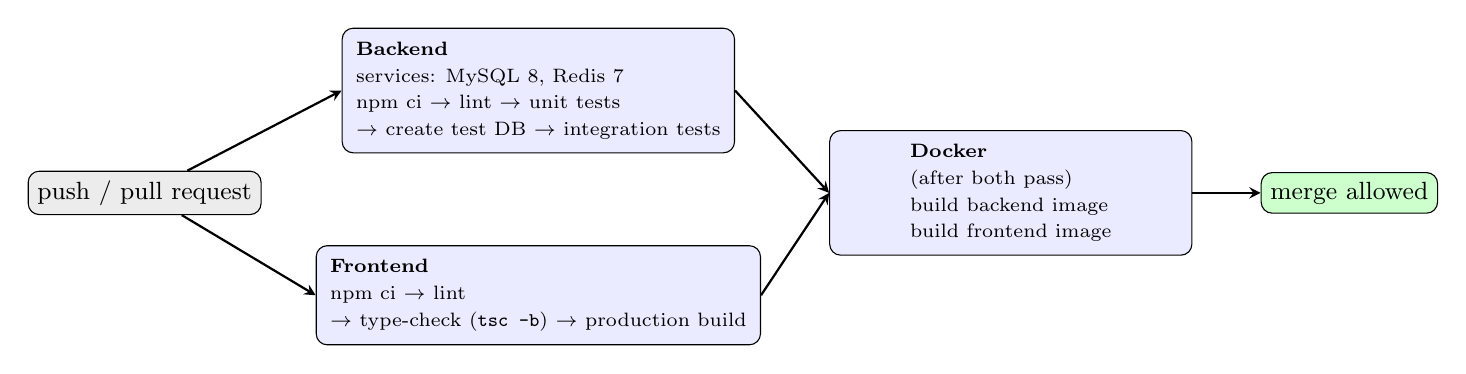
\begin{tikzpicture}[
  job/.style={draw, rounded corners, fill=blue!8, minimum width=4.6cm, align=left, font=\scriptsize, inner sep=5pt},
  arr/.style={->, >=stealth, thick}
]
\node[draw, fill=gray!15, rounded corners, font=\small] (push) at (0,0) {push / pull request};
\node[job] (be) at (5,1.3) {\textbf{Backend}\\services: MySQL 8, Redis 7\\npm ci $\rightarrow$ lint $\rightarrow$ unit tests\\$\rightarrow$ create test DB $\rightarrow$ integration tests};
\node[job] (fe) at (5,-1.3) {\textbf{Frontend}\\npm ci $\rightarrow$ lint\\$\rightarrow$ type-check (\texttt{tsc -b}) $\rightarrow$ production build};
\node[job] (dk) at (11,0) {\textbf{Docker}\\(after both pass)\\build backend image\\build frontend image};
\node[draw, fill=green!20, rounded corners, font=\small] (ok) at (15.3,0) {merge allowed};
\draw[arr] (push) -- (be.west);
\draw[arr] (push) -- (fe.west);
\draw[arr] (be.east) -- (dk.west);
\draw[arr] (fe.east) -- (dk.west);
\draw[arr] (dk) -- (ok);
\end{tikzpicture}%
}
\caption{Continuous Integration Pipeline (GitHub Actions)}
\label{fig:ci}
\end{figure}

The backend job runs the full unit and integration suites against real MySQL and Redis service containers, so the integration test that needs Redis also runs there. At present the frontend job lints, type-checks and builds the application; the Vitest and Playwright suites are run locally before each pull request. Adding them to the pipeline is listed as future work.

\FloatBarrier
\section{Test Results}

Table~\ref{tab:testsummary} in Chapter~\ref{ch:impl} summarises the results: all 165 backend unit tests, all 126 frontend tests, all 80 integration tests and all 12 end-to-end tests pass. ESLint reports no errors in either project, and the TypeScript compiler reports no type errors.

\FloatBarrier
\section{Defects Found and Fixed}

Table~\ref{tab:defects} lists the most significant defects found by the tests, reviews and mutation testing during this phase, and how each was fixed. Each fix is accompanied by a regression test.

\begin{longtable}{|C{0.8cm}|L{4.3cm}|L{3.9cm}|L{4.2cm}|}
\caption{Significant Defects Found and Fixed} \label{tab:defects} \\
\hline
\rowcolor{blue!12}
\textbf{No.} & \textbf{Defect} & \textbf{Impact} & \textbf{Fix} \\
\hline
\endfirsthead
\hline
\textbf{No.} & \textbf{Defect} & \textbf{Impact} & \textbf{Fix} \\
\hline
\endhead
D1 & MediBot replies were inserted into the page as HTML without escaping & Cross-site scripting through prompt injection & Escaping Markdown renderer with a link-scheme whitelist; protocol-relative \texttt{/\textbackslash host} also blocked \\
\hline
D2 & Payment could be started for an appointment whose time had passed & Patients charged for visits that can no longer happen & Server rejects orders more than 60 minutes after the start; \texttt{can\_pay} flag hides the button \\
\hline
D3 & Admin payments list returned every row & Slow page and large responses as data grows & Validated \texttt{page}/\texttt{limit} with \texttt{LIMIT/OFFSET}, total count and pager \\
\hline
D4 & Only application code prevented a second open bed allocation & A race or future code path could double-book a bed & Unique \texttt{open\_bed\_id} and \texttt{open\_patient\_id} keys; duplicate-key errors mapped to 409 \\
\hline
D5 & Database session ran in UTC while slot times are stored in IST & \texttt{NOW()} comparisons 5.5 hours off on cloud servers & Session time zone pinned to +05:30 on every pooled connection \\
\hline
D6 & \texttt{JOIN ... FOR UPDATE} and locks on missing rows & Deadlocks under concurrent admissions and payments & Split locked and unlocked reads, fixed lock order, deadlock retry in \texttt{inTransaction} \\
\hline
D7 & Test for the payment-fail endpoint did not check ownership effects & A removed ownership check would go unnoticed & Assertion that another patient's request leaves the order unchanged \\
\hline
D8 & Jest did not exit after the integration suite & CI jobs hang until timeout & Each test file closes its database pool and Redis client \\
\hline
D9 & Backend kept running when its port was already in use & Silent failure in development and deployment & Process exits with an error if the port cannot be bound \\
\hline
D10 & Development script depended on an uninstalled tool (nodemon) & \texttt{npm run dev} failed on a fresh clone & Uses Node's built-in \texttt{node --watch} \\
\hline
D11 & Prescription files were public static files under \texttt{/uploads}, typed by file name & Anyone with the URL could read another patient's prescription; files lost on restart & Files stored in MySQL, served only to the patient and doctor, type checked by content \\
\hline
D12 & Cancelling did not free the slot (\texttt{slot\_id} was unique) and three cancel paths differed & Cancelled slots were lost; paid cancellations not flagged & One cancel service; \texttt{active\_slot\_id} unique key; \texttt{refund\_due}; other side notified \\
\hline
D13 & MediBot booked through its own endpoint & Past and blocked slots could be booked from the chat & Chat uses \texttt{/api/\allowbreak appointments/\allowbreak book} and lists only bookable slots \\
\hline
D14 & Blocking a day deleted its slots & The midnight generator recreated them, reopening the day & Slots are marked unavailable instead \\
\hline
D15 & Deleting a user or appointment cascaded to payments & Loss of financial records & \texttt{ON DELETE RESTRICT} and a clear 409 \\
\hline
D16 & Nightly cleanup deleted past free slots that cancelled visits still pointed to & Visit history deleted, or cleanup failed on a paid visit and skipped slot generation & Keep referenced slots; cleanup and generation fail independently \\
\hline
D17 & Two first requests raced for the CSRF cookie, and the cookie ended with the browser & Random 403 errors, and logouts, for returning users & Cookie lives as long as the refresh token; \texttt{CSRF\_INVALID} code; one client retry \\
\hline
D18 & One trusted proxy hop behind Vercel and Render; successful logins counted & All visitors shared one rate-limit bucket: 10 logins per 15 minutes for the whole site & \texttt{TRUST\_PROXY\_HOPS=2}; only failures count; extra per-account limit \\
\hline
D19 & Visits could be completed or prescribed long before they started, and slots created for any date & Wrong records; unbounded slot rows & 15-minute rule; booking and slot window of today plus 13 days \\
\hline
D20 & Admin lists loaded every row and counted on the client & Slow pages and wrong dashboard totals as data grew & Server-side filtering, search, sorting and paging \\
\hline
\end{longtable}


\chapter{Deployment and Operations}
\label{ch:deploy}
\lhead{\emph{Chapter 7: Deployment and Operations}}
\FloatBarrier
\section{Deployment Architecture}

The first version ran only on the developers' laptops. In this phase the system was deployed to the cloud using free tiers of managed services, as shown in Figure~\ref{fig:deploy}. The React application is built into static files and served by Vercel's content delivery network. Vercel also rewrites every \texttt{/api/*} request to the backend, so from the browser's point of view the frontend and the API share one origin and the session cookies are first-party. The backend runs as a Docker container on Render, next to Render's managed Redis, and the database is a managed MySQL~8 service on Aiven, reached over TLS with the provider's CA certificate verified. Behind the rewrite every request passes two proxies (Vercel, then Render), which is why the backend is configured to trust exactly two proxy hops when it reads the client's IP address for rate limiting. Uploaded files live in the database, so the backend container holds no state and can be replaced at any time.

\begin{figure}[H]
\centering
\resizebox{\textwidth}{!}{%
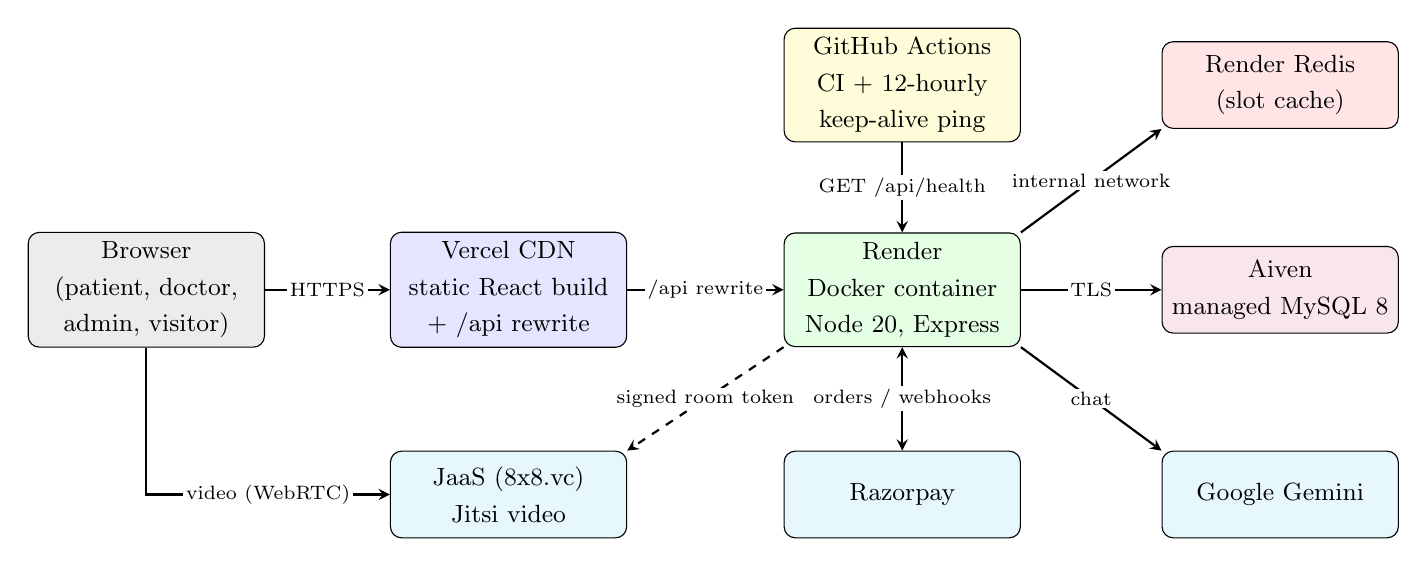
\begin{tikzpicture}[
  box/.style={draw, rounded corners, minimum width=3.0cm, minimum height=1.1cm, align=center, font=\small},
  arr/.style={->, >=stealth, thick},
  lbl/.style={font=\scriptsize, fill=white, inner sep=1pt}
]
\node[box, fill=gray!15] (user) at (0,0) {Browser\\(patient, doctor,\\admin, visitor)};
\node[box, fill=blue!10] (vercel) at (4.6,0) {Vercel CDN\\static React build\\+ /api rewrite};
\node[box, fill=green!10] (render) at (9.6,0) {Render\\Docker container\\Node 20, Express};
\node[box, fill=red!10] (redis) at (14.4,2.6) {Render Redis\\(slot cache)};
\node[box, fill=purple!10] (aiven) at (14.4,0) {Aiven\\managed MySQL 8};
\node[box, fill=cyan!10] (rzp) at (9.6,-2.6) {Razorpay};
\node[box, fill=cyan!10] (gem) at (14.4,-2.6) {Google Gemini};
\node[box, fill=cyan!10] (jit) at (4.6,-2.6) {JaaS (8x8.vc)\\Jitsi video};
\node[box, fill=yellow!15] (gha) at (9.6,2.6) {GitHub Actions\\CI + 12-hourly\\keep-alive ping};
\draw[arr] (user) -- node[lbl]{HTTPS} (vercel);
\draw[arr] (vercel) -- node[lbl]{/api rewrite} (render);
\draw[arr] (render) -- node[lbl]{TLS} (aiven);
\draw[arr, <->] (render) -- node[lbl]{orders / webhooks} (rzp);
\draw[arr] (render.south east) -- node[lbl]{chat} (gem.north west);
\draw[arr] (user.south) |- node[lbl, pos=0.75]{video (WebRTC)} (jit.west);
\draw[arr, dashed] (render.south west) -- node[lbl]{signed room token} (jit.north east);
\draw[arr] (render.north east) -- node[lbl]{internal network} (redis.south west);
\draw[arr] (gha) -- node[lbl]{GET /api/health} (render);
\end{tikzpicture}%
}
\caption{Production Deployment Architecture}
\label{fig:deploy}
\end{figure}

\FloatBarrier
\section{Containerisation}

Both applications have a Dockerfile, and a \texttt{docker-compose.yml} file starts the complete stack locally (MySQL~8, Redis~7, the backend and the frontend served by Nginx) with one command. The backend image is based on \texttt{node:20-alpine}, installs only production dependencies with \texttt{npm ci --omit=dev} (in a separate layer so that it is cached), installs time-zone data, sets \texttt{TZ=Asia/Kolkata}, and runs \texttt{start.sh}. The image needs no volume: prescription files and doctor photos are stored in MySQL, because Render's free plan wipes the container's disk on every restart. Nginx (local stack) and Vercel (production) add the same security headers to the frontend that the API sets on its responses. The CI pipeline builds both images on every change, which guarantees that they always build.

\FloatBarrier
\section{Database Migrations on Start-up}

Render's free plan offers no shell for running one-off commands, so migrations are applied automatically. On every start, \texttt{start.sh} runs the migration script, which applies \texttt{schema.sql} and every migration file through the idempotent runner described in Chapter~\ref{ch:impl}, and then starts the server. A failed migration is logged but does not stop the server: if the database is briefly unreachable at boot, the API still starts, reports \texttt{database: "disconnected"} from its health endpoint, and recovers once the database is back, instead of crash-looping.

\FloatBarrier
\section{Configuration and Secrets}

All configuration is supplied through environment variables, and no secret is committed to the repository. Table~\ref{tab:env} lists the main variables. The Render blueprint (\texttt{render.yaml}) declares them with \texttt{sync: false} so that their values are entered in the dashboard. A separate \texttt{.env.test} file configures the test database, so tests can never touch development or production data.

\begin{longtable}{|L{5.3cm}|L{8.3cm}|}
\caption{Main Environment Variables} \label{tab:env} \\
\hline
\rowcolor{blue!12}
\textbf{Variable} & \textbf{Purpose} \\
\hline
\endfirsthead
\hline
\textbf{Variable} & \textbf{Purpose} \\
\hline
\endhead
NODE\_ENV & \texttt{production} enables Secure/SameSite=None cookies and hides error details \\
\hline
PORT & HTTP port (5001 by default in development) \\
\hline
DB\_HOST, DB\_PORT, DB\_USER, DB\_PASSWORD, DB\_NAME & Database connection \\
\hline
DB\_SSL, DB\_CA\_CERT & TLS to the managed database and the provider's CA certificate for verification \\
\hline
JWT\_SECRET, JWT\_REFRESH\_SECRET & Signing keys for access and refresh tokens \\
\hline
ACCESS\_TOKEN\_TTL\_MIN, REFRESH\_TOKEN\_TTL\_DAYS & Token lifetimes (15 minutes and 7 days by default) \\
\hline
CORS\_ORIGIN & Allowed frontend origin for credentialed CORS requests \\
\hline
GEMINI\_API\_KEY & MediBot \\
\hline
REDIS\_HOST, REDIS\_PORT, REDIS\_PASSWORD & Optional cache; the system works without it \\
\hline
TZ & Must be \texttt{Asia/Kolkata} (Section~\ref{sec:tz}) \\
\hline
TRUST\_PROXY\_HOPS & Proxies in front of the API (default 1; 2 on Render behind Vercel) \\
\hline
RAZORPAY\_KEY\_ID, RAZORPAY\_KEY\_SECRET, RAZORPAY\_WEBHOOK\_SECRET & Payment gateway and webhook verification \\
\hline
PAYMENT\_MODE & \texttt{mock} explicitly allows the mock gateway outside development \\
\hline
JAAS\_APP\_ID, JAAS\_KID, JAAS\_PRIVATE\_KEY & JaaS application, API key id and private key used to sign room tokens \\
\hline
JITSI\_DOMAIN & Jitsi server used when the JaaS keys are empty (default \texttt{meet.jit.si}, which no longer allows embedding; local testing only) \\
\hline
\end{longtable}

\FloatBarrier
\section{Time Zone Handling}
\label{sec:tz}

Appointment slots are stored as a \texttt{DATE} and a \texttt{TIME} column in Indian Standard Time, and many queries compare them with \texttt{NOW()} (for example the join window and the past-appointment check). Cloud servers, however, usually run in UTC. If the Node.js process and the MySQL session used different zones, ``now'' would be 5.5 hours off and patients could be refused, or allowed, at the wrong times. The system therefore sets the zone consistently in three places: the Docker image sets \texttt{TZ=Asia/Kolkata} for the Node.js process, every pooled MySQL connection runs \texttt{SET time\_zone = '+05:30'} before any other query (the offset form needs no time-zone tables on the server), and date arithmetic that must not drift, such as blood expiry dates, is done in UTC on plain date strings. Integration tests create appointments relative to the database's own \texttt{NOW()} so that they behave the same on any machine.

\FloatBarrier
\section{Health Check and Keep-Alive}

\texttt{GET /api/health} returns the API status together with the result of a real database query. Render uses it as the container health check. Aiven's free MySQL tier powers off after about a day without queries, so a scheduled GitHub Actions workflow calls the health endpoint every 12 hours, which both keeps the database active and fails loudly if the deployment is down.

\FloatBarrier
\section{Demonstration Data}

For demonstrations and evaluation, the command \texttt{npm run db:seed-demo} fills the database so that the system looks as it would after some months of use, while respecting every rule of the application. Using the doctors already in the database, it adds 60 patients, two months of past appointments with prescriptions, ratings, payments and cancellations, bookings for the next ten days, blood donors, stock and requests, extra wards with admitted patients, pending bed and discharge requests, and an active emergency board. A second step gives the existing patients about five months of visits with detailed prescriptions (diagnosis, medicines, advice and follow-up) and attaches a one-page prescription PDF on hospital letterhead to nearly every prescription. The seed runs in one transaction, runs only once (demo patients use the reserved domain \texttt{demo.example.com}), keeps booked slots, booking limits, paid video visits and bed occupancy consistent, and refuses to run with \texttt{NODE\_ENV=production} unless \texttt{--yes} is given.

\FloatBarrier
\section{Production Readiness Checklist}

The deployed system runs with test keys and free-tier services. Table~\ref{tab:readiness} lists what must be done before it is used by a real hospital.

\begin{longtable}{|C{0.7cm}|L{6.0cm}|L{6.8cm}|}
\caption{Production Readiness Checklist} \label{tab:readiness} \\
\hline
\rowcolor{blue!12}
\textbf{No.} & \textbf{Item} & \textbf{Reason} \\
\hline
\endfirsthead
\hline
\textbf{No.} & \textbf{Item} & \textbf{Reason} \\
\hline
\endhead
1 & Switch Razorpay to live keys and subscribe the webhook to \texttt{payment.captured}, \texttt{order.paid} and \texttt{payment.failed} & Payments made after the browser is closed are recorded only through the webhook \\
\hline
2 & Issue refunds through the Razorpay Refunds API & Cancelled paid visits are currently only flagged \texttt{refund\_due}; the refund is made by hand in the dashboard \\
\hline
3 & Set the three \texttt{JAAS\_*} keys (or run a self-hosted Jitsi server) under an agreement suitable for clinical data & Without them video falls back to \texttt{meet.jit.si}, which cannot be embedded and is not meant for clinical use \\
\hline
4 & Change the passwords of, or remove, the default demo accounts that \texttt{schema.sql} creates (password \texttt{password}) & They are public in the repository and recreated on start-up if missing \\
\hline
5 & Check \texttt{bed\_allocations} for duplicate open stays before running the bed migration on an existing database & The new unique keys cannot be created while duplicates exist \\
\hline
6 & Move files from MySQL to object storage (e.g. S3) as their number grows & Keeps the database small; the free Aiven tier has 1~GB \\
\hline
7 & Never run the demo data seed against real data & It adds 60 fictitious patients; with \texttt{NODE\_ENV=production} it refuses to run without \texttt{--yes} \\
\hline
8 & Upgrade from free tiers & Free instances sleep when idle, causing slow first requests \\
\hline
9 & Add monitoring and alerting (metrics, error tracking) & Today there are request logs and a health check only \\
\hline
\end{longtable}


\chapter{Conclusions and Future Work}
\label{ch:conclude}
\lhead{\emph{Chapter 8: Conclusions and Future Work}}
\section{Conclusions}

The present project work has introduced Care \& Cure HMS – an extensive end-to-end solution of Hospital Management System which caters to the deficiencies of open-source and academic HMS solutions available currently – and has extended it from an out-patient appointment system into a hospital digital ecosystem. Conclusions drawn from the project work are:

\textbf{Role-Based Architecture:} The solution has been able to successfully implement the three-role based architecture (Patient, Doctor, Administrator), together with a public visitor experience, with the use of middleware and enforcing strong access control policy such that users cannot access anything beyond their designated role due to JWT based token verification and role checking middleware implementation. Multi-role guards allow doctors and administrators to share clinical modules while ownership checks keep each patient's records, including prescription files, private, and the principle of least privilege is applied to beds: doctors request, the administrator assigns.

\textbf{Dynamic Appointment Engine:} The specialization-based appointment booking, along with availability checking of slots at real time and transactional level double booking prevention using database locking technique with the use of a \texttt{UNIQUE} constraint on \texttt{active\_slot\_id}, has resulted in an efficient and race condition-free appointment engine which generates 14-day slots automatically. Appointments can now be in person or by video, can be cancelled by any party with the slot freed and paid visits flagged for refund, are limited per patient so that no account can hoard the schedule, and the availability lookups are cached.

\textbf{AI Integration:} The MediBot chat bot, powered by the Google Gemini API, has shown that large language models are able to follow constraints imposed by prompt engineering in order to execute deterministic actions. The natural language + action block approach implemented has made conversation with the MediBot more friendly, and its output is now rendered safely so that a manipulated reply cannot run code in the user's browser.

\textbf{Comprehensive Admin Control:} The Admin Dashboard has provided an exhaustive feature set which enables the administrator to manage user accounts as well as appointment slots in a granular fashion, and now also wards and beds, the blood bank, the emergency board, the navigation map and the payments ledger. This solves a typical problem associated with academic HMS where there is lack of any or rudimentary administrator feature sets.

\textbf{Security:} The combination of bcrypt password hashing, JWT based authentication in httpOnly cookies with short-lived access tokens and refresh rotation, CSRF double-submit tokens, Zod validation of every input, rate limiting, parameterized SQL queries, file type validation, signed and idempotent payment webhooks, and a restrictive CORS policy has provided proper security features to make the web app ready for live deployment.

\textbf{Hospital Operations Modules:} The seven new modules show that clinical rules can be encoded directly and verifiably in software: ABO/Rh compatibility and first-expiry-first-out issue in the blood bank, the five-level Emergency Severity Index in the emergency department, a timed and payment-gated join window and a doctor-controlled waiting room for video consultations, and Dijkstra's shortest-path algorithm for step-free indoor navigation.

\textbf{Data Integrity under Concurrency:} Combining row locks in a fixed order, a deadlock-retrying transaction helper and database unique keys as the final guard has made bed admission, blood issue, booking and payment safe under concurrent use, which was demonstrated by tests that fire conflicting requests simultaneously.

\textbf{Quality and Delivery:} The original 15 manual functional tests have been replaced by 383 automated tests at four levels, checked by mutation testing and two code audits and run in a continuous integration pipeline, and the system has been containerised and deployed to the cloud.

All the 15 function test cases of the first version and the 40 new functional test cases have successfully passed, along with all automated tests, indicating that all aspects of the implementation have worked as expected.

\section{Future Work}

Two items proposed as future work in the first report, \emph{Online Payment Gateway} and \emph{Telemedicine Extension}, have been implemented in this phase, and \emph{Real-time Messaging} has been partly addressed by in-app notifications. A few possible extensions to further increase the functionality of Care \& Cure HMS include:

\begin{enumerate}
    \item \textbf{Real-time Messaging and Delivery Channels:} Pushing notifications and waiting-room updates instantly with WebSockets (Socket.IO) instead of polling, and delivering them by e-mail and SMS (for example with Nodemailer and Twilio), would enhance patient engagement and make emergency alerts reach staff who are away from the screen.

    \item \textbf{Integration with EHR Standards:} To ensure that the HMS can interact with other health information technologies, adding interoperability features using standards like HL7 FHIR would be useful.

    \item \textbf{Admin Analytics Dashboard:} Adding visualizations to the admin dashboard using chart libraries (like Chart.js and Recharts) will enable data-driven decision-making within hospitals, for example bed occupancy trends, emergency waiting times by ESI level, blood stock and wastage, and revenue.

    \item \textbf{Mobile App:} Creating a mobile app using React Native or Flutter will further enhance the system's usability by providing patients with a mobile application.

    \item \textbf{Advanced MediBot:} The chatbot can be enhanced by adding persistent memory capabilities and integrating external drug and symptom checking APIs for richer guidance. However, proper safety warnings should be provided before giving any clinical advice.

    \item \textbf{Multi-Hospital System:} Extending the database and overall HMS infrastructure to enable multi-hospital operations and department-specific management would enable the system to function across multiple hospital branches.

    \item \textbf{Laboratory and Radiology Module:} Ordering tests, recording results and attaching reports to the patient's history would close the last gap identified in the comparison with existing hospital systems.

    \item \textbf{In-patient Billing and Pharmacy:} Combining bed charges (the daily rate is already stored), procedures, medicines and consultation fees into a single bill, and issuing the refunds that are now only flagged through the Razorpay Refunds API.

    \item \textbf{Blood Bank Extensions:} Cross-match records, donor eligibility questionnaires, barcode labels for units, and transfer of stock between hospitals.

    \item \textbf{Richer Navigation:} A visual floor map with the route drawn on it, QR codes at junctions to set the starting point, and A* search if the map grows large.

    \item \textbf{Full Test Automation in CI:} Running the Vitest and Playwright suites in the GitHub Actions pipeline, adding code-coverage reporting, and automated mutation testing with a tool such as Stryker.

    \item \textbf{Audit Trail and Compliance:} An immutable log of who viewed or changed clinical and financial records, data retention policies, and alignment with India's Digital Personal Data Protection Act, 2023 before handling real patient data.
\end{enumerate}

\section{Limitations}

The current system has the following limitations, which should be considered before deployment in a real hospital:

\begin{itemize}
    \item \textbf{Stateless refresh tokens.} Refresh tokens are rotated but not stored on the server, so a stolen refresh token cannot be revoked before it expires (at most 7 days). A token store or token version per user would allow forced logout.
    \item \textbf{Triage is a suggestion only.} The ESI level is computed from the inputs the clinician enters and must always be confirmed by a trained clinician; the system does not replace clinical judgement.
    \item \textbf{Single-hospital, single-time-zone design.} Slot times are stored in IST and the system assumes one hospital.
    \item \textbf{Free-tier hosting.} The deployed instance sleeps when idle, keeps uploaded files in the free 1~GB database, and runs with test payment keys (see Table~\ref{tab:readiness}).
    \item \textbf{Manual refunds and polling.} Refunds are flagged but issued by hand, and the waiting room and notifications use polling (every 5 and 30 seconds) rather than push messages.
    \item \textbf{Public default accounts.} The demonstration administrator and doctor accounts have a published password and must be changed before real use.
    \item \textbf{Comparison data.} The comparison with Jaipur hospitals in Chapter~\ref{ch:literature} is based on publicly available information collected for the first report and has not been re-verified.
    \item \textbf{No real-user evaluation.} The system has been validated through automated and manual testing by the team, not through a usability study with patients and hospital staff.
\end{itemize}


%% ----------------------------------------------------------------
\appendix
\chapter{Installation and Setup Guide}
\label{app:setup}
\lhead{\emph{Appendix A: Installation and Setup Guide}}
\section{Prerequisites}

\begin{itemize}
    \item Node.js 20 or later and npm.
    \item MySQL 8 (or MariaDB 10.4+, for example through XAMPP or MAMP).
    \item Optional: Redis 7 for caching, Docker and docker-compose for the containerised setup, and Google Chrome for the end-to-end tests.
    \item A Google Gemini API key for MediBot. Razorpay test keys are optional: without them, payments run in mock mode in development.
\end{itemize}

\section{Running Locally}

\begin{lstlisting}[language=bash, caption=Backend Setup]
cd backend
npm install
cp .env.example .env      # set DB_*, JWT_SECRET, JWT_REFRESH_SECRET, GEMINI_API_KEY
npm run db:migrate        # applies schema.sql and all migrations
npm run dev               # API on http://localhost:5001
node seedData.js          # optional: more sample doctors and slots
npm run db:seed-demo      # optional: demo patients, visits, beds, blood (runs once)
\end{lstlisting}

\begin{lstlisting}[language=bash, caption=Frontend Setup]
cd frontend
npm install
npm run dev               # http://localhost:5173, proxies /api to :5001
\end{lstlisting}

\section{Running with Docker}

\begin{lstlisting}[language=bash, caption=Complete Stack with docker-compose]
cp backend/.env.example backend/.env   # fill in secrets
docker-compose up --build              # MySQL, Redis, backend, frontend
# open http://localhost:8080 ; migrations run automatically on start
\end{lstlisting}

\section{Running the Tests}

\begin{lstlisting}[language=bash, caption=Test Commands]
cd backend
npm test                  # unit tests (no database needed)
npm run test:integration  # creates hms_db_test and runs integration tests
npm run lint

cd ../frontend
npm test                  # Vitest component and contract tests
npm run test:e2e          # Playwright; starts backend (mock payments) and Vite
npm run lint && npm run build
\end{lstlisting}

The integration and end-to-end tests need a local MySQL whose credentials are in \texttt{backend/.env.test}; the test database name must contain \texttt{test}, because it is dropped and recreated. Redis is optional; only the cache test needs it. Variables already set in the shell take precedence over \texttt{.env.test}, so a different local password can be passed as \texttt{DB\_PASSWORD=... npm run test:integration}.

\section{Deploying}

\begin{enumerate}
    \item Create a MySQL service on Aiven and note its host, port, user, password and CA certificate.
    \item On Render, create a Blueprint from the repository; \texttt{render.yaml} defines the Docker web service. Enter the database variables (with \texttt{DB\_SSL=true}), the JWT secrets, \texttt{GEMINI\_API\_KEY}, \texttt{CORS\_ORIGIN}, \texttt{TRUST\_PROXY\_HOPS=2}, the Razorpay keys (without them payments and video bookings are disabled in production) and the three \texttt{JAAS\_*} keys for embedded video. The Blueprint also creates the Redis instance.
    \item On Vercel, import the \texttt{frontend} folder. \texttt{vercel.json} rewrites \texttt{/api} to the Render URL and sets the security headers; \texttt{VITE\_BACKEND\_URL} must stay unset so that the rewrite is used.
    \item In the GitHub repository, set the \texttt{BACKEND\_HEALTH\_URL} variable to the Render URL followed by \texttt{/api/health} to enable the keep-alive workflow.
\end{enumerate}


\chapter{User Guide by Role}
\label{app:ui}
\lhead{\emph{Appendix B: User Guide by Role}}
This appendix describes the main screens available to each type of user and the order in which they are typically used.

\section{Visitor}

\begin{itemize}
    \item \textbf{Home (\texttt{/})}: hospital information, specialities and a link to sign in or register.
    \item \textbf{Find your way (\texttt{/navigate})}: choose ``From'' and ``To'' locations, optionally tick \emph{step-free route}, and read the numbered directions with the floor and distance of each step.
    \item \textbf{MediBot}: the chat button at the bottom right opens the assistant, which can suggest a speciality for described symptoms and list doctors. Booking through MediBot requires signing in as a patient and follows the same rules as the booking page.
\end{itemize}

\section{Patient}

\begin{enumerate}
    \item \textbf{Register and sign in} (\texttt{/login}).
    \item \textbf{Book an appointment} (\texttt{/patient/book}): choose a speciality, a doctor, a date within the next 14 days and a free 15-minute slot, select \emph{In person} or \emph{Video}, add a reason and confirm. A notification confirms the booking. A patient can hold up to five upcoming visits, and one per doctor per day.
    \item \textbf{My appointments} (\texttt{/patient/history}): see upcoming and past visits, pay the consultation fee with the \emph{Pay} button, join a paid video visit with the \emph{Join} button from 15 minutes before the start and wait there until the doctor admits you, cancel an upcoming visit before it starts (a paid visit is refunded), open prescription files, and rate completed visits.
    \item \textbf{Payments} (\texttt{/patient/payments}): history of all payments with status and reference numbers.
    \item \textbf{Medical records} (\texttt{/patient/records}) and \textbf{Profile} (\texttt{/patient/profile}).
    \item \textbf{Notifications}: the bell icon shows unread alerts; clicking one opens the related page.
\end{enumerate}

\section{Doctor}

\begin{enumerate}
    \item \textbf{Dashboard}: today's schedule and counts of pending and completed appointments.
    \item \textbf{Appointments} (\texttt{/doctor/appointments}): complete a visit from 15 minutes before its start or cancel it, open video consultations, admit the waiting patient and mark the consultation completed, and upload prescriptions (\texttt{/doctor/prescribe}).
    \item \textbf{Emergency} (\texttt{/doctor/emergency}): register an arrival with vital signs, accept or override the suggested ESI level, work the queue from the top, assign, treat, discharge or transfer, and press \emph{Request bed} when the patient must be admitted.
    \item \textbf{Beds} (\texttt{/doctor/beds}): see ward occupancy, request a bed for a patient (ward type, urgency, reason), follow your requests, see the beds of your admitted patients and request their discharge.
    \item \textbf{Blood bank} (\texttt{/doctor/blood}): check stock by group and component, raise a request for a patient with an urgency, and cancel own pending requests.
\end{enumerate}

\section{Administrator}

\begin{enumerate}
    \item \textbf{Dashboard}: hospital-wide statistics.
    \item \textbf{Doctors, Patients, Appointments, Slots}: create and edit doctor accounts with a profile photo, search and page through patients and appointments, cancel or complete visits, toggle individual slots, block whole days and regenerate slots.
    \item \textbf{Beds} (\texttt{/admin/beds}): create wards and beds, put free beds into maintenance or reserve them, work the \emph{Requests} tab (assign a bed, approve a discharge, or reject with a reason), and admit walk-in patients from the bed grid, where beds with a requested discharge are highlighted.
    \item \textbf{Blood bank} (\texttt{/admin/blood}): register donors, record donations, view and discard units, and fulfil or reject requests.
    \item \textbf{Emergency} (\texttt{/admin/emergency}): the same board as doctors, alerts for ESI level 1 and 2 arrivals and emergency bed requests, and direct admission to a bed.
    \item \textbf{Payments} (\texttt{/admin/payments}): ledger of all payments with totals, 50 per page, including cancelled paid visits marked \emph{refund due}.
    \item \textbf{Navigation map}: add or remove locations and connections through the navigation API.
\end{enumerate}


%% ----------------------------------------------------------------
\addtotoc{Bibliography}
\addtocontents{Bibliography}{\vspace{2em}}
\newpage
\lhead{\emph{Bibliography}}
\nocite{*}
\small{\bibliography{bibch1}{}}
\bibliographystyle{ieeetr}

\end{document}
